%\documentclass[final,fmstyle,twoside,openright]{./util/ucathesis}
\documentclass[final,fmstyle]{./util/ucathesis}

\usepackage[T1]{fontenc}
\usepackage[spanish]{babel}
\usepackage[utf8]{inputenc}
\usepackage{csquotes} 
\usepackage{graphicx}
\usepackage[showframe=false, left=40mm, right=20mm]{geometry}
\usepackage[inline]{enumitem}
\usepackage{pgfgantt}
\usepackage[bookmarks]{hyperref}
\usepackage{changepage}
\usepackage{booktabs}
\usepackage{listings}
\usepackage{xcolor}
\usepackage{colortbl}
\usepackage{xargs}
\usepackage{rotating}
\usepackage{tkz-kiviat}
\usepackage{multirow}
\usepackage[normalem]{ulem}
\usepackage{pdflscape} % Ver si no funciona con páginas en formato de tesis http://goo.gl/Rszezu
%\usepackage{rotating}
\usepackage{tabulary}
\usepackage{titlesec}
\usepackage[newcommands]{ragged2e}
\usepackage{pdfpages}
\usepackage{pgfplots}
\usepackage{tikz}
\usepackage{tkz-kiviat}
\usepackage[style=numeric,sorting=none,backend=biber]{biblatex}
\usepackage{glossaries}
\usepackage{etoolbox}
\usepackage[xindy]{imakeidx}
%\usepackage[colorinlistoftodos,prependcaption,spanish]{todonotes}
\usepackage{filecontents}
\usepackage{util/pgf-pie}

\newcommand{\removed}[1]{\uline{#1}}
\newcommand{\tabitem}{~~\llap{\textbullet}~~}

\pgfdeclarelayer{background}
\pgfdeclarelayer{foreground}
\pgfsetlayers{background,main,foreground}
\usetikzlibrary{shapes,arrows,shadows}

% PACKAGE titlesec
\setcounter{secnumdepth}{4}

\titleformat{\paragraph}
{\normalfont\normalsize\bfseries}{\theparagraph}{1em}{}
\titlespacing*{\paragraph}
{0pt}{3.25ex plus 1ex minus .2ex}{1.5ex plus .2ex}

% END PACKAGE titlesec

% Agregar bullets al entorno description
\setlist[description]{font=\quad$\bullet\enskip$\bfseries}


\DeclareUnicodeCharacter{00E3}{á}



\tikzstyle{block} = [rectangle, draw, fill=gray!20, 
    text width=10em, text centered, rounded corners, minimum height=4em]
\tikzstyle{line} = [draw, -latex']

%\MakePerPage{footnote}
\addbibresource{bibliography.bib} 

%Datos de la tesís
\title{Juegos serios como apoyo a la formación de profesionales: \protect\\ Una aplicación al 
área de  enfermería}
\author{Mirta Beatriz González Leguizamón y Arturo Pedro Volpe Torres}
\degree{Informática}

\advisor{Ing.}{Martín Abente Lahaye, M.Sc.}

\logosource{./util/logo.pdf}
\institution{Universidad Nacional de Asunción}
\faculty{Facultad Politécnica}
\address{San Lorenzo - Paraguay}

%% templates
\lstdefinestyle{sharpc}{language=[Sharp]C, frame=lr, rulecolor=\color{blue!80!black}}

\newtoks\customtok


\renewcommand*{\newacronymhook}{%
 \edef\dosetkeys{\noexpand\setkeys{glossentry}{user1={},\the\glskeylisttok}}%
 \dosetkeys
 \ifcsempty{@glo@useri}%
 {%
   \expandafter\customtok\expandafter{\the\glsshorttok}%
 }%
 {%
   \edef\custom{\the\glsshorttok, \csexpandonce{@glo@useri}}%
   \expandafter\customtok\expandafter{\custom}%
 }%
}

\newcommand*{\custompostdesc}[1]{%
  \ifcsempty{glo@#1@useri}{}{(\glsentryuseri{#1})}%
}

\renewcommand*{\CustomAcronymFields}{%
  user1={},%
  name={\the\glsshorttok},%
  description={\the\glslongtok\noexpand\custompostdesc{\the\glslabeltok}},%
  first={\the\glslongtok\space(\the\customtok)},%
  firstplural={\the\glslongtok\noexpand\acrpluralsuffix\space(\the\customtok)}%
  text={\the\glsshorttok},%
  plural={\the\glsshorttok\noexpand\acrpluralsuffix}%
}

%\newcommandx{\todox}[2][1=]{\todo[linecolor=gray,backgroundcolor=white,#1]{#2}}
%\newcommandx{\martin}[2][1=]{\todo[linecolor=blue,backgroundcolor=white,#1]{#2}}
%\newcommandx{\replantear}[2][1=]{\todo[inline,caption={Replantear},#1]{#2}}
%\newcommandx{\observacion}[2][1=]{\todo[inline,caption={Observacion},#1]{#2}}
%\newcommandx{\pregunta}[2][1=]{\todo[backgroundcolor=white,inline,caption={Pregunta},#1]{¿#2?}}
%\newcommandx{\revisar}[2][1=]{\todo[size=\small,caption={Revision},linecolor=red,backgroundcolor=white,#1]{#2}}
%\newcommand{\tabletodo}[2][]{\begin{minipage}{3cm}\todo[inline,#1]{#2}\end{minipage}}
%\newcommand{\fixme}[2]{\uline{#1}\todo[linecolor=blue,backgroundcolor=green,size=\small]{#2}}
%\newcommand{\cs}{C$\sharp$ }
%\newcommand{\cs}{C\includegraphics{hash-symbol}}
\newcommand{\cs}{%
  {\settoheight{\dimen0}{C}C\kern-.05em \resizebox{!}{\dimen0}{\raisebox{\depth}{\fontseries{b}\selectfont\#}}}}

% COLOR para las tablas
\definecolor{gris}{gray}{0.85}
\definecolor{agua}{rgb}{0.88,1,1}

\SetCustomStyle
\makeglossaries
\makeindex

\begin{document}


\newacronym[user1=Conseil Européen pour la Recherche Nucléaire]{cern}{CERN}{Organización Europea para la Investigación Nuclear}
\newacronym[user1=One Laptop Per Child]{olpc}{OLPC}{Una computadora por niño}
\newacronym[user1=Massachusetts Institute of Technology]{mit}{MIT}{Instituto Tecnológico de Massachusetts}
\newacronym{tic}{TIC's}{Tecnologías de la información y la comunicación}
\newacronym[user1=Event-Condition-Action]{eca}{ECA}{acciones condicionadas por eventos}
\newacronym{iab}{IAB}{Instituto Andrés Barbero}
\newacronym[user1=Graphics Processing Unit]{gpu}{GPU}{Unidad de procesamiento de gráficos}
\newacronym[user1=Application Programming Interface]{api}{API}{Interfaz de programación de aplicaciones }



\maketitle

%! TEX root = ../main.tex
\chapter*{Agradecimientos}

Al \textbf{Ing. Martín Abente Lahaye}, por su orientación  y tiempo dedicado
durante el desarrollo de este trabajo de grado.

A la \textbf{Dirección de la carrera de Licenciatura en Enfermería del Instituto
    Doctor Andrés Barbero}, por su valioso aporte, tanto de directores como
profesores, sin el cual no habría sido posible el desarrollo y la aplicación de
este trabajo de grado.
 
A la \textbf{Facultad Politécnica de la Universidad Nacional de Asunción}, por
la formación académica recibida durante los años de carrera, la cual nos alienta
a ser excelentes profesionales.

A los \textbf{Profesores de la carrera de Ingeniería en Informática}, quienes
colaboraron de varias maneras para el desarrollo de este trabajo y nos brindaron
apoyo durante el camino para alcanzar la meta.

A nuestros \textbf{Amigos y Compañeros}, quienes durante los años de carrera
universitaria nos brindaron su apoyo durante los momentos buenos y los momentos
difíciles.

A nuestras \textbf{Familias}, quienes nos inspiran a seguir adelante y nos
acompañan en cada paso dado a lo largo de nuestra vida. Un agradecimiento
especial al esfuerzo y entrega dados durante todos estos años.

A \textbf{Dios}, sin cuya bendición nada de esto hubiese sido posible.

% Tabla de contenidos
%\setcounter{secnumdepth}{5}
%\setcounter{tocdepth}{5}
\tableofcontents
% Lista de figuras
\listoffigures
% Lista de tablas
\listoftables
% Lista de algoritmos
\listofalgorithms

%\listoftodos
%\todototoc

\printglossary[type=\acronymtype,title=Lista de Siglas]

\addcontentsline{toc}{chapter}{Lista de Siglas}

\mainmatter

%! TEX root = ../main.tex
\chapter{Introducción}


En la actualidad, la educación tradicional o instruccionismo se basa en el
concepto de que el profesor transfiere el conocimiento que ha adquirido de
diferentes métodos (educación, experiencia, etc.) a un alumno que es un receptor
pasivo de información\cite{laptop:instructionism}. 

En la educación tradicional el uso de las \Gls{tic} cumplía con un rol en el 
cual sólo eran un mecanismo más para transmitir el conocimiento del maestro al alumno,
reemplazando libros y presentaciones. Actualmente, el uso de las tecnologías tiene un
papel más activo dentro del proceso de aprendizaje.

Además del instruccionismo existen otras corrientes pedagógicas relacionadas a
las \Gls{tic}, entre las que se pueden citar el conductismo, el constructivismo
y el construccionismo. Este trabajo se centra en el construccionismo.

El construccionismo tiene un enfoque diferente en cuanto a las \Gls{tic} ya que
utiliza la tecnología como un mecanismo de adquisición de conocimiento y no como
una herramienta proveedora del mismo\cite{sasha:construtivism}, es decir se
centra en como se generan los conocimientos y no en como proveer información
previamente establecida. 

Algunos de los proyectos que incluyen al construccionismo son: 
el lenguaje de programación LOGO, las simulaciones educativas de entornos virtuales, 
los juegos serios y Lego Serious Play.

El aprendizaje apoyado por las \Gls{tic} y el construccionismo utilizando
específicamente los juegos serios tienen la capacidad de eliminar los problemas
de distancia, en el ámbito empresarial se utilizan los juegos serios para
enseñar a grupos de personas a trabajar en equipo, incluso cuando estos se
encuentran a distancias que le impiden reunirse en una clase
tradicional\cite{mariluz:seiousgames}, es así que estudios anteriores han
demostrado que el construccionismo es una alternativa muy prometedora al
instruccionismo\cite{sasha:construtivism}.
   
De los proyectos citados anteriormente, la simulación es una opción tecnológica
propicia para el construccionismo ya que permite utilizar la exploración y el
ensayo para desarrollar habilidades y pericias en entornos
controlados\cite{humphreys2013developing}. La simulación puede ser complementada
con la utilización de juegos serios ya que los mismos proveen una oportunidad
muy importante para enseñar y desarrollar profesionales\cite{sg:aoverview}.

Basándonos en lo explicado anteriormente, se considera interesante el campo de
investigación que involucra el desarrollo de aplicaciones tecnológicas que
ayuden a estudiantes en el proceso de aprendizaje. 

Estas herramientas tienen especial importancia en ambientes donde las
limitaciones, de espacio, y tiempo dificultan la aplicación de técnicas
tradicionales. Uno de estos casos es el entrenamiento de profesionales de
Enfermería los cuales requieren de varias horas de práctica durante su
preparación, y la misma se realiza en instituciones como hospitales escuela,
donde los alumnos son supervisados por profesionales mientras realizan las
prácticas.

Además, según \cite{humphreys2013developing} los alumnos de enfermería, son
estudiantes divergentes, es decir aprenden a través de experimentación activa, e
interiorizan el conocimiento reflexionando sobre la experiencia. La simulación
es una herramienta ideal para este tipo de
estudiantes\cite{humphreys2013developing}.

Teniendo en cuenta que los mismos forman parte de un grupo de profesionales que
requieren de un alto grado de prácticas y que en la actualidad se presentan
varios factores que a un estudiante de esta carrera le impide poner a prueba
todo el tiempo sus conocimientos y por todo lo expuesto anteriormente, en este
trabajo se propone el desarrollo de un juego serio, que involucra la simulación
de laboratorios virtuales, como una herramienta para el proceso de aprendizaje
de los alumnos de la carrera de enfermería.

%! TEX root = ../main.tex
\section{Objetivo General}
\label{sec:objetivos_generales}

Realizar una investigación sobre el rol actual de las tecnologías de la
información y la comunicación en la educación, poniendo énfasis en las 
corrientes pedagógicas actuales, y evaluar las distintas tecnologías 
disponibles para introducirlo en un área especifica.

% Enfoque 3.89
%El objetivo general de la presente tesis es investigar, estudiar y evaluar 
%las diferentes tecnologías disponibles para apoyar el proceso de aprendizaje 
%utilizando como base pedagógica el construccionismo para  diseñar un esquema 
%de desarrollo que se pueda implementar en el área de enfermería. 
%\observacion{Creo que es la segunda vez que pregunto. Pero lo de enfermería es un
%    caso de prueba, no es el objetivo general (ver correcciones generales)}


% Enqoue NEGATIVO
% \fixme{diseñar e implementar un
    %aplicación}{No puede ser un objetivo general!} 
%estudiar y evaluar tecnologías que permitan  apoyar el
%proceso de aprendizaje de los alumnos de la carrera de enfermería, utilizando
%como base pedagógica el construccionismo.


% Enfoque 1
%% Diseñar un esquema de desarrollo de tecnologías que permitan complementar el
%% proceso de aprendizaje de los alumnos de la carrera de enfermería, utilizando
%% como base pedagógica el construccionismo.

% Enfoque 2
%% Investigar, estudiar y evaluar las aplicaciones de juegos serios 
%% construccionistas como herramientas complementarias a la educación tradicional.
\section{Objetivos Específicos}

Con el fin de aproximarnos a nuestro propósito, se formulan los siguientes
objetivos específicos:

\begin{enumerate}
    \item Proveer un resumen de los fundamentos y estado actual de la corriente
        \emph{Construccionismo}, como herramienta pedagógica y su relación con
        las \gls{tic}.
        % Proveer un resumen de los fundamentos y estado del arte de las
        % corrientes actuales relacionadas con las \gls{tic}.

    \item Proveer un resumen actualizado acerca de los juegos serios y
        corrientes afines como herramientas para la aplicación del
        construccionismo.
    
    \item Proveer un resumen actualizado de las áreas de aplicabilidad de los
        juegos serios, poniendo énfasis en las áreas que permiten un enfoque
        construccionista.
        
    \item Identificar las características del área de enfermería que hacen que
        la misma sea un contexto factible para la aplicación de los juegos
        serios basados en el construccionismo.
    
    \item Analizar, evaluar y seleccionar las herramientas que nos permitan la
        implementación de un juego serio que simule un laboratorio de
        enfermería.
        
    \item Diseñar e implementar un juego serio construccionista que permita
        exponer las ventajas y desventajas como modelo de apoyo a la enseñanza
        tradicional. 
        %\observacion{Recuerden tener/exponer las ventajas y desventajas en la
        %    conclusión}

    \item Evaluar la solución propuesta para la obtención de datos que permitan
        medir las fortalezas y debilidades desde el punto de vista del usuario,
        en cuanto a factores de:
        \begin{enumerate*}[label=\itshape\alph*\upshape)]
            \item exploración,
            \item representación,
            \item motivación,
            \item inmersión,
            \item utilidad,
            \item retroalimentación, y,
            \item pedagogía.
        \end{enumerate*}

    \item Identificar las fortalezas y debilidades de los métodos utilizados
        para definir su aplicabilidad como herramienta de apoyo. 

    \item Identificar desde el ámbito del diseño, desarrollo y evaluación los puntos que deben
        tenerse en cuenta a la hora de implementar este tipo de herramientas de
        apoyo.
\end{enumerate}

\section{Estructura del libro}
    

%\fixme{A continuación se explica el proceso que fue realizado para alcanzar los objetivos citados 
%    anteriormente, las etapas de este proceso se presentan en diferentes capítulos los cuales 
%    tratan de diversos aspectos.}{Borrar}

% TIC's en la educación
%En el capitulo~\ref{chap:tics} se expande el estado actual de las \Gls{tic} en
%la educación, desde sus inicios, las expectativas creadas, los progresos
%realizados, y las experiencias, la evolución de la teoría hasta hoy en día.

En el capítulo~\ref{chap:tics} se presenta un resumen sobre el uso de las
\Gls{tic} en la educación, desde sus inicios apoyando a la educación
tradicional hasta su rol actual en las nuevas corrientes pedagógicas. Se
hace énfasis en la corriente pedagógica llamada construccionismo, explicando
su historia, base pedagógica, el rol y la forma de uso de las \Gls{tic} en
la misma.

% Juegos serios
%En el capitulo~\ref{chap:juegos_serios} se describen las características y áreas de aplicación de un 
%juego serio, incluyendo corrientes relacionadas y algunos casos de éxito. Se muestra 
%además un esbozo de como desarrollar un juego serio.

En el capítulo~\ref{chap:juegos_serios} se describen a los juegos serios, siendo 
estos una de las herramientas tecnológicas usadas dentro del proceso de aprendizaje, 
se detallan sus características, áreas de aplicación, las corrientes tecnológicas relacionadas, 
y el proceso de desarrollo además de describir algunos casos de éxito. También se describen 
tecnologías relacionadas a los juegos serios.


% Definición del problema

En el capítulo~\ref{chap:problema} se definen las características del problema
que se quiere abordar para darle una solución tecnológica. Enfocándonos en el
área de enfermería se describe la situación actual y una propuesta de solución tecnológica 
que puede brindar apoyo en el proceso de aprendizaje.



%nseñanza utilizado en el \Gls{iab}, enfocado específicamente a la carrera de
%Licenciatura en Enfermería, la distribución de los cursos, carga horaria,
%prácticas de laboratorio y prácticas en hospitales, así como los mecanismos de
%evaluación utilizados.

%Además se citan los problemas existentes, como las dificultades que tienen los
%alumnos en los distintos aspectos que influyen en la vida de un estudiante, y
%problemas inherentes a la enseñanza de profesiones técnicas con métodos de
%enseñanza tradicionales. Y por último se describen los procedimientos de enfermería 
%en los que se enfocará este trabajo.


% Hipotesis y requerimientos de la solucion

En el capítulo \ref{chap:requerimientos} se definen los criterios que deben tenerse en 
cuenta para seleccionar el contenido a abordar en la solución, se seleccionan y describen 
los procedimientos de enfermería que formarán parte del contenido, el alcance  
y los requisitos que debe cumplir la solución.

%En el capítulo~\ref{chap:requerimientos} se describen los requisitos que deben 
%tenerse en cuenta para el desarrollo de la solución propuesta, incluyendo las hipótesis asumidas
%con respecto a diferentes aspectos de los procedimientos de enfermería.

%Tecnologías utilizadas

En el capítulo~\ref{chap:tecnologias} se describen las diversas tecnologías utilizadas 
en el desarrollo del proyecto, haciendo especial énfasis en los motores de juego ya que 
los mismos proveen el entorno principal para el desarrollo de la solución, se realiza 
una comparación entre los motores de juegos actuales y se justifica por que se seleccionó 
uno en específico. 


% Propuesta de solución

%El capitulo~\ref{chap:solucion} describe una solución  para la aplicabilidad de juegos serios 
%en un contexto con las características mencionadas en el capitulo anterior utilizando los conceptos
%estudiados en el capítulo~\ref{chap:tics}, se proponen, además, consideraciones
%a tener en cuenta referentes a los componentes e interacción entre los mismos.

%Así mismo se definen mecanismos para tratar con los limites de una simulación, y
%como utilizar las herramientas descritas en el capítulo~\ref{chap:tics} en
%armonía con los objetivos pedagógicos.

En el capítulo~\ref{chap:solucion} se describe en detalle la solución propuesta basada en 
la aplicabilidad de los juegos serios en un contexto con las características mencionadas en 
el capítulo~\ref{chap:problema} y teniendo en cuenta las requisitos detallados en el 
capítulo~\ref{chap:requerimientos} haciendo uso de las tecnologías descritas en el capítulo 
anterior. 

% Definición de evaluación

Dada la solución propuesta, en el capítulo~\ref{chap:evaluacion} se propone una
forma de evaluarla, teniendo en cuenta las hipótesis planteadas durante su
desarrollo  y los objetivos del presente trabajo. Esta evaluación consiste en
una serie de pruebas, se define el universo, la muestra, y los criterios de
selección de la muestra.

% Análisis de resultados

Se presentan además los resultados de las diferentes
pruebas llevadas a cabo, obtenidos en forma tabular y con gráficos para
facilitar la comprensión. %Además se estudian factores de correlación entre las
%distintas variables medidas.

% Conclusiones

En el capítulo~\ref{chap:conclusion} se presentan las
conclusiones obtenidas a partir de los resultados obtenidos y la experiencia
adquirida durante el desarrollo de la solución.

% Trabajo furuto

Finalmente, en el capítulo~\ref{chap:futuro} se describen algunos trabajos posibles que pueden
ser desarrollados en el área teniendo en cuenta el presente trabajo. 

%\observacion{Volver a revisar más adelante}


\chapter{TIC en la educación}

Las \Gls{tic} son un conjunto de herramientas tecnológicas y recursos utilizados
para comunicar, crear, diseminar, almacenar y manejar la
información\cite{unesco:ict}. Estas tecnologías abarcan computadoras personales,
internet, radio, televisión y telefonía\cite{tinio:ict}.

Las \Gls{tic} fueron utilizadas como complemento a la educación desde los
inicias de la misma con la radio y la televisión. Fueron vistas como un
complemento a las herramientas utilizadas en clase, como complemento del libro,
o como una herramienta que elimina la distancia física entre el profesor y el
alumno\cite{unesco:ict}. 

La utilización de las \Gls{tic} no mostró una utilidad clara hasta la
utilización masiva de las computadoras, es en esta área donde se encontraron los
resultados más prometedores\cite{unesco:ict}. 

Las principales ventajas de la utilización de las \Gls{tic} en la educación es
su aplicabilidad en áreas que no pueden ser cubiertas por otras alternativas,
como son:

\begin{description}

    \item[Nuevos modelos pedagógicos] teorías como el constructivismo moderno
	    enfatizan el proceso de como adquirir conocimiento y no solamente el
	    conocimiento en sí.

    \item[Recursos remotos] Las herramientas tradicionales como las bibliotecas,
	    escuelas y universidades están limitadas a un espacio físico, con
	    las \Gls{tic} este requerimiento físico desaparece, prueba de ello
	    es el Internet, que es la colección más grande de información y esta
	    disponible prácticamente a cualquier estudiante\cite{tinio:ict}.

    \item[Colaboración distribuida] como consecuencia del punto anterior, los
	    alumnos pueden colaborar de manera más sencilla pues no tienen
	    limitaciones físicas. Además, los alumnos pueden consultar con
	    expertos que están en linea, e incluso tener mentores en linea,
	    estas tutorías pueden ser uno a uno, por ejemplo mediante
	    comunicaciones por correo electrónico. Además permite la
	    colaboración masiva entre estudiantes de intereses comunes, mediante
	    foros y redes sociales\cite{unesco:ict}.

    \item[Motivación para aprender] la utilización de contenido multimedia puede
	    ayudar a que los alumnos deseen involucrarse más en el proceso
	    educativo.

    \item[Adquisición de habilidades básicas] las habilidades necesarias para
	    utilizar de manera efectiva las \Gls{tic} se están convirtiendo en
	    una necesidad básica, un aprendizaje guiado por las mismas puede
	    ayudar a una rapida asimilación de los conceptos relacionados.

\end{description}

Uno de los desafíos más importantes que enfrentan las \Gls{tic} para convertirse
en una alternativa viable es la inversión en infraestructura
necesaria\cite{unesco:ict}. 

\section{Historia de las TIC en la educación}

La historia de las \Gls{tic} en educación comienza con la Universidad Abierta
del Reino Unido\footnote{Open University of United Kingdom} que en 1969 se
establece como la primera institución educativa dedicada a la enseñanza a
distancia utilizando las, para aquel entonces, nuevas
tecnologías\cite{tinio:ict}.

En 1973 Vint Cerf creo el protocolo TCP/IP y es considerado el nacimiento de
Internet\cite{white:ict}, lo que permitió que la información pueda ser
transmitida de manera más sencilla, tiempo después con la aparición de las
computadoras personales en 1977\cite{white:ict}. 

Otro hito tecnológico se dio en la \Gls{cern} en el año 1989 cuando se concibió
lo que hoy se conoce como \emph{World Wide Web}, permitiendo que los usuarios de
la \emph{Web} puedan compartir archivos mediante un protocolo
estándar\cite{white:ict}. 

Con las principales eventos que marcaron la evolución tecnológica de las
\Gls{tic} en la educación, se divide su historia en cinco partes. Las mismas se
pueden dividir en dos secciones, las primeras tres corresponden a los comienzos
y donde los alumnos eran receptores de información, época denominada, y la
segunda denominada\emph{push}\cite{white:ict} que es aquella donde los alumnos
participan de su educación y son creadores activos de conocimiento.

\subsection{Programación, ejercicios y prácticas}

Este periodo que abarca desde la aparición de las primeras computadoras
personales hasta el final de la década de 1980, este periodo se caracterizo por
computadoras muy limitadas, nula interacción multimedia y escasez de programas
especializados. Se enseñaba programación básica\cite{leinonen:ict}, no por la
necesidad de educar programadores, sino por la creencia de que así se
desarrollarían habilidades matemáticas y lógicas en los alumnos. Los programas
eran muy simples y se basaban en matemáticas y nociones básicas del idioma. 

Esta clase de ejercicios no ayudaron a los alumnos a obtener un aprendizaje
profundo, pues era fácil resolverlos a través de la prueba y el error, la mayor
parte del tiempo servían para distraer a los alumnos no interesados en la
programación mientras el profesor enseñaba programación a aquellos que parecían
interesados\cite{leinonen:ict}.


\subsection{Entrenamiento basado en computadoras}

Cuando aparecieron en el mercado computadoras con multimedia, se argumento que
los ejercicios de la era anterior fallaron en su objetivo de una educación
profunda por que no contenían multimedia\cite{leinonen:ict}, las aplicaciones
eran distribuidas por CD-ROM, y así se actualizaban de manera más frecuente, y
podían contener gran cantidad de contenido multimedia.

En este periodo se desarrollaron una gran cantidad de aplicaciones educativas
que más tarde serían conocidas como \emph{Edutainment}\footnote{Education +
	Enteirtainment, se traduce como educación entretenida}, estas pretendían
agregarle entretenimiento a la educación, se veía al como un receptor pasivo de
información que debía asimilarla, y para aumentar el compromiso, el
entretenimiento era agregado\cite{resnick:2004}.

Las bases pedagógicas de esta se basada en la capacidad de ciertos estudiantes
de aprender mejor cuando interactúan con contenido multimedia, la \emph{prueba y
	error} aún estaban presentes, pero no eran presentados inmediatamente,
sino más bien una vez que el alumno ya debería haber asimilado los conceptos y
funcionaban como pruebas de adquisición de conocimiento. Este tipo de contenido
tampoco logro la enseñanza profunda, solamente fueron efectivos en el
aprendizaje de idiomas, fallando en todos los demás campos\cite{leinonen:ict},
además los contenidos muchas veces estaban desactualizados y obtener nuevas
versiones no era una tarea sencilla.

Varios gobiernos apoyaron de manera agresiva la introducción de las \Gls{tic} en
educación\cite{mcdougall2006theory} y se realizo un importante avance teórico
con los trabajos sobre el aprendizaje construccionista de Papert y Harel (1991),
y la influencia de las computadoras sobre el aprendizaje y la mente de Marvin
Minksy (1987)~\cite{mcdougall2006theory}.

A comienzos de la decada de 1990, con la popularización de Internet, se le vio
como solución al problema de las poco frecuentes actualizaciones de aplicaciones
educativas, su utilización no tenia bases pedagógicas, más bien se basaban en la
facilidad de distribuir contenido por la \emph{Web}, el principal inconveniente
era la velocidad del Internet, no era suficiente para proveer entornos ricos en
multimedia como lo hacían los CD-ROM\cite{leinonen:ict}.

\subsection{e-Learning}

La bases pedagógicas de esta son similares a la era del entrenamiento basado en
computadoras, se distribuye contenido masivamente a los alumnos, y luego, de
manera muy discreta se permite a los mismos colaborar, dejando siempre en claro
que primero se debe asimilar toda la información posible y luego relacionarse
con los demás\cite{leinonen:ict}.

El \emph{e-Learning} apareció a finales de la década de 1990 y tubo su apogeo en
mediados de la década del 2000, apoyada por la gran penetración de las \Gls{tic}
en la población\cite{punie:ict}.

Todos los paradigmas anteriores viven dentro del \emph{e-Learning}, permitiendo
compartir contenido multimedia y realizar pruebas del tipo \emph{prueba-error}. 

Si bien en las anteriores épocas, el uso de las \Gls{tic} estaba más orientado
hacia la educación básica y secundaría, el \emph{e-Learning} actualmente es más
utilizado en la educación terciaría\cite{punie:ict}.

La utilización del \emph{e-Learning} tiene varios grados de aplicación en
entornos reales\cite{punie:ict}, que van desde ser simples elementos
complementarios a la clase, como por ejemplo un repositorio para las
diapositivas y otros materiales de clase, hasta cursos completamente en linea,
donde la clase ha sido completamente sustituída.


%\input{tics/arte}
\section{Problemas actuales}
\label{tics:problemas}

Durante la historia de las \Gls{tic} en la educación, se han encontrado
diferentes dificultades a la hora de aplicar los nuevos conceptos en la
educación, desde los primeros enfoques que carecían de bases pedagógicas válidas
hasta la actualidad.

El principal problema es falta de motivación de los profesionales de la
educación para emplear las \Gls{tic}\cite{punie:ict}\cite{ict:romeo}.

El contenido proveído actualmente puede ser considerado como un conjunto de
buenas prácticas\cite{punie:ict} y así, omiten completa o parcialmente el
contexto donde esa buena práctica fue generado.

A la hora de educar a los educadores en la utilización de las \Gls{tic} no se
debe medir medidas cuantitavias, como las notas o el número de cursos, sino más
bien el impacto cualitativo de la educación

Las \Gls{tic} han tenido un impacto positivo en la educación\cite{punie:ict},
pero no han obtenido el impacto esperado.

Iniciativas como el \emph{Edutainment}, prometían ser la solución a los
problemas educacionales, sin embargo, su implementación no cumplio con las
expectativas, obtuvieron una reputación negativa, y hoy en día son considerados
como el peor tipo de educación, pues son un ejercicio de \emph{prueba-error}
ocultos bajo un juego poco entretenido\cite{resnick:2004}. La principal critica
contra los \emph{Edutainment} es su incapacidad de enseñar como aplicar
conceptos aprendidos a un entorno real\cite{resnick:2004}.

Mientras que la utilización de las \Gls{tic} puede eliminar problemas actuales
como el aislamiento y la falta de pensamiento de alto nivel\cite{punie:ict}, la
brecha social existente implica otro riesgo para la utilización de las \Gls{tic}
en la educación, aquellos que no posean los recursos económicos necesarios para
acceder a la misma no se verán beneficiados por las \Gls{tic}\cite{punie:ict}.


 

\section{Construccionismo y las TIC's}
\label{sec:tics_CONSTRUCCIONISMO}

El construccionismo es una corriente pedagógica que parte de una concepción del
aprendizaje según la cual la persona aprende por medio de su interacción
dinámica con el mundo físico, social y cultural en el que está
inmerso\cite{valdivia:sg}.

Posee un enfoque diferente en cuanto al uso de las \Gls{tic} en la educación.
Esta pedagogía se diferencia de la educación tradicional en que el estudiante ya
no es un receptor pasivo de información, en cambio, el mismo participa
activamente del proceso de aprendizaje construyendo su propio conocimiento. Se
diferencia del instruccionismo en que el construccionismo utiliza la tecnología
como medio cognitivo y no para la entrega de contenido.

Se considera al construccionismo como una alternativa prometedora a la educación
tradicional. Desde el punto de vista tecnológico, es ideal pues el mismo
requiere un alto dinamismo en el traspaso del conocimiento
\cite{sasha:construtivism}. 

El construccionismo y las \Gls{tic} siempre han estado relacionados, ya que el
mismo se originó con un lenguaje de programación (LOGO)\cite{ict:ttc}. Un
característica importante de esta relación es que tienen la capacidad de
eliminar los problemas de distancia\cite{mariluz:seiousgames}.


\subsection{Historia}

A mediados de la década de 1960 Seymour Papert, un matemático sudafricano, llegó
a los Estados Unidos, donde fue co-fundador del Laboratorio de Inteligencia
Artificial del \Gls{mit} con Marvin Minsky\cite{logo:sg}. 


En la década de $1980$, Seymour Papert acuñó el término construccionismo en la
Fundación Nacional de Ciencia de los Estados Unidos titulada
\enquote{Constructionism: A New Opportunity for Elementary Science Education}
para presentar un método pedagógico que se basaba en muchas de las ideas de la
educación progresiva estudiadas por el estadounidense John Dewey en el inicio
del siglo 20 en su escuela experimental en la Universidad de Chicago. Dewey
quería poner gran parte de la responsabilidad de aprender en los estudiantes que
han nacido con el don de aprendizaje y la creación de conocimiento en sus
propios términos\cite{historia:2014}.

Papert también fue influenciado por Maria Montessori quien luego de grados en
pediatría, medicina, psicología y filosofía comenzó su propia escuela
experimental para niños pequeños. En lugar de que ella misma estableciera
formalmente las tareas, vio como sus estudiantes actuaron por su cuenta. Ella
siguió los intereses de los estudiantes y observó como respondieron a sus
entornos especialmente preparados. Ella preparó el escenario pero no ofreció una
guía explícita\cite{historia:2014}.

Papert trabajó directamente con el psicólogo suizo Jean Piaget a quien Ernst von
Glasersfeld llamó \enquote{El pionero de la teoría constructivista del
    aprendizaje}. 
% esto de glaserfeld pio importa?
Piaget, al igual que Dewey, Montessori y otros, desarrolló su teoría de la
educación y la construcción del conocimiento observando e interactuando con los
niños. De estas observaciones nació el movimiento constructivista. El
contructivismo se basa en que el conocimiento debe ser construído por el
estudiante y los nuevos significados deben ser obtenidos relacionándolos a
significados anteriores en el propio sistema de relaciones del
estudiante\cite{historia:2014}. 

Papert admitió que jugó más con la palabra construcción. El contruccionismo de
Papert se diferencia del constructivismo de Piaget en que los estudiantes
construyen las ideas o partes del mundo utilizando herramientas. Para Papert los
estudiantes necesitan contruir modelos de partes de su mundo con el fin de
comprender más plenamente el significado, el 
% la definición de modelos podemos poner un footnote?
contenido y la dinámica de las partes. La elaboración de representaciones
mentales mediante la construcción y el intercambio es la metáfora del marco
construccionista\cite{historia:2014}.

%Durante $1980$, Seymor Papert, Wally Feurzeig, Marvin Minsky y John McCarthy y los
%miembros del Departamento de Inteligencia Artificial del \Gls{mit} y una
%compañía de tecnología en Cambridge, Massachusetts, desarrollaron un nuevo
%lenguaje de programación llamado LOGO que tenía por objeto que los estudiantes
%construyeran sus modelos mentales en notación LOGO. Este juego
%introduciría de forma natural las ideas de los procedimientos, funciones,
%variables, recursividad, la modularidad, simulación, verificación, entre %otros\cite{historia:2014}.

Papert trabajó con el equipo de Bolt, Beranek y Newman, liderado por Wallace
Feurzeig, que creó la primera versión del lenguaje de programación LOGO en 1967.
LOGO es un dialecto de Lisp, fue diseñado como una herramienta para el
aprendizaje. Sus características, como la modularidad, extensibilidad,
interactividad y flexibilidad, derivan de este objetivo \cite{logo:sg}.

Los desarrolladores de LOGO no solo alentaron la promoción de formas
construccionistas de enseñanza y aprendizaje sino también alentaron otra forma
de aprendizaje nueva y no tradicional con las diferentes herramientas
tecnológicas\cite{historia:2014}. 

Por lo tanto, se puede decir que la creación de LOGO permitió la creación del
construccionismo\cite{historia:2014}.

    
    
% ESTE
% Cuando se produjo LOGO y se acuñó el construccionismo, la comunidad del 
% construccionismo era en su mayoría ingenieros informáticos y matemáticos\cite{historia:2014}.
% Esto es relevante?

\observacion{Toda la sección hay que reordernar}

\subsection{Bases Pedagógicas}

Para el construccionismo, el conocimiento es construido por el estudiante en
lugar de ser trasmitido por el profesor \cite{moses:2003} y esto sucede particularmente cuando
el mismo se compromete en la elaboración de un producto o artefacto que tenga un
significado y pueda ser compartido\cite{valdivia:sg}. De esta manera, se permite
a los estudiantes elaborar sus propias interpretaciones razonadas del mundo
mediante la interacción con el mismo. El profesor actúa como guía para el estudiante 
en la construcción de su conocimiento, aportando conocimiento y experiencia.

Según Papert, los alumnos estarán mucho más involucrados en su aprendizaje si
construyen artefactos que los demás pueden ver, criticar y tal vez utilizar. Y
además, el alumno se enfrenta a problemas complejos con estas construcciones,
harán el esfuerzo por resolver problemas y aprender ya que la construcción les
motivará\cite{const:vs}.

El enfoque construccionista establece que los seres humanos conocen y aprenden
de formas diferentes por lo tanto, no se puede elaborar una jerarquía de estilos
de aprendizajes\cite{valdivia:sg}.

\subsection{Actualidad}

%El construccionismo pone énfasis en el \emph{Aprender haciendo}, esta idea
%\fixme{mejora}{ref} la práctica educativa tradicional o instruccionismo. %El instruccionismo
%se basa en el concepto de que existe un profesor y un estudiante, el profesor
%transfiere el conocimiento que ha adquirido a un alumno que es receptor pasivo
%de información de esta manera, se enfoca más en la capacidad del profesor. 

Existen varios proyectos o emprendimientos que incluyen al contruccionismo como
base pedagógica, para la mayoría de ellos las computadoras son esenciales
mientras que para otros el mayor esfuerzo está en la incorporación de la
tecnología en su práctica educativa\cite{papertian:const}.

Algunos de estos emprendimientos son:

\begin{itemize}

\item \textbf{Lenguaje de programación LOGO}: El lenguaje LOGO es la cuna del construccionismo. %, se basa en el
%	principio de que se aprende mejor haciendo, pero se aprende todavía
%	mejor si se combina la acción con la verbalización  y la reflexión
%	acerca de lo que se ha hecho. 
	Fundamentalmente consiste en presentar a
	los niños retos intelectuales que puedan ser resueltos mediante el
	desarrollo de programas en LOGO. El proceso de revisión manual de los
	errores contribuye a que el niño desarrolle habilidades metacognitivas
	al poner en práctica procesos de auto-corrección\cite{logo:sg}.
	%http://es.wikipedia.org/wiki/Logo_(lenguaje_de_programaci%C3%B3n)


    %A mediados de la década de 1960 Seymour
	%Papert, que había estado trabajando con Piaget en Ginebra, llegó a
	%Estados Unidos donde co-fundó el Laboratorio de Inteligencia Artifical
	%del MIT con Marvin Minsky. Papert trabajó con el equipo de Bolt, Beranek
	%y Newman, liderado por Wallace Feurzeig, que creó la primera versión del
	%logotipo en 1967. A lo largo de la década de 1970 Logo fuen incubado en
	%el MIT y algunos otros sitios de investigación. El lenguaje de
	%programación Logo, un dialecto de Lisp, fue diseñado como una
	%herramienta para el aprendizaje. Sus características como la
	%modularidad, extensibilidad, interactividad y flexibilidad se derivan de
	%este objetivo. 
	%http://el.media.mit.edu/logo-foundation/logo/index.html

    Las actividades de programación LOGO se realizan en las áreas de matemática, lenguaje, 
    música, robótica, telecomunicaciones y ciencias. LOGO es accesible para novatos, 
    incluyendo niños pequeños, y también es compatible con exploraciones complejas y 
    proyectos sofisticados realizados por usuarios experimentados\cite{logo:sg}.
    
    Uno de los ambientes más populares de LOGO incluye a la tortuga, originalmente 
    era un robot que era puesto en el suelo y se podía dirigir su movimiento 
    escribiendo comandos en el ordenador. Pronto la tortuga emigró a las 
    pantallas gráficas de los ordenadores en donde se las utiliza para dibujar 
    formas y diseños\cite{logo:sg}.

    

%\item[Simulación] La simulación en el ámbito de la educación fue evolucionando
%desde simples motores de reglas hasta complejos entornos, la simulación
%demostró ser una herramienta muy útil el ámbito laboral
%\cite{mariluz:seiousgames}, pues enseña al alumno a encarar situaciones muy
%difíciles de representar en entornos completamente controlados y provee
%mecanismos para comprobar la efectividad de la herramienta. 

%Actualmente la simulación se utiliza más en el ámbito empresarial pues las
%empresas son las más necesitas de innovar en el ámbito de la enseñanza. Un
%ejemplo de esta necesidad se da, por ejemplo, en el entrenamiento de nuevos
%vendedores, es muy difícil enseñar a un vendedor como debe vender los productos
%con un pizzarón y/o una presentación, en cambio la simulación permite que el
%mismo pueda probar cosas nuevas y experiencias de sus compañeros (o
%instructor), convirtiendo así el aprendizaje en
%colectivo\cite{mariluz:seiousgames}. En el ámbito académico la simulación mas
%utilizada en campos físicos (como simulación de fluidos), meteorología
%(simulación de tormentas y fenómenos climáticos), etc. 

%\item[Serious Games] Diseñado con el propósito de aprender. Generalmente hace
%uso de la simulación para permitir un aprendizaje más realista.

%\item[Lego Serious Play] Es una iniciativa de Lego que busca fomentar el
%pensamiento creativo por medio de la construcción por parte de los estudiantes
%de su identidad y experiencias utilizando legos. 

\item \textbf{\Gls{olpc}}: es una asociación sin ánimos de lucro cuyo esfuerzo
    se centra en dotar a los niños de una computadora duradera, accesible y
    potente en los países en desarrollo, se dice que es un descendiente directo
    del construccionismo\cite{papertian:const}.
	
    Surgió dentro del MIT Media Lab, \Gls{olpc} propone un cambio de paradigma
    basado en un modelo de aprendizaje en el que cada alumno disponga de su
    propia computadora portátil y que se pueda conectar a internet, de forma
    totalmente gratuita, desde su escuela. A partir de esta política se pretende
    disminuir la brecha tecnológica y de acceso de información en países más
    desfavorecidos en comparación con los países del primer
    mundo\cite{videojuegos:gonzaleztardon}.
	
	%Con esto se busca que
	%la computadora personal sea utilizada como un laboratorio intelectual y
	%un vehículo para la auto-expresión. OLPC no tiene que ver con la
	%escolarización o la escuela, más bien las utiliza como medio de
	%distribución de las computadoras a los niños, los cuales pueden
	%utilizarlas para aprender en cualquier lugar y momento. Se busca
	%fomentar el aprendizaje natural, es decir, aquel aprendizaje sin
	%enseñanza.

    %\fixme{Los problemas atribuidos al experimento}{experimento?} OLPC son
    %predominantemente las críticas a la política, el liderazgo o de la
    %intransigencia de la escuela en vez del construccionismo o computadora
    %personal para los niños pobres. El experimento audaz de Nicholas Negroponte
    %(co-fundador de \Gls{olpc}) y Sugata Mitra para dejar las computadoras desde
    %un helicóptero sobre una aldea de África se basa en la creencia en el
    %construccionismo\cite{papertian:const}.

\item \textbf{Fabricación personal}: Neil Gershenfeld, colega de Papert en el
    Media Lab del \Gls{mit} dictó un curso titulado \emph{Cómo hacer casi
        cualquier cosa}. La idea se centraba en la creación de  la tecnología
    que se necesita para resolver los problemas que se poseen. Esta
    auto-confianza, la autonomía personal y la agencia sobre la tecnología han
    estado en el centro de trabajo de Papert durante años. Papert no sólo
    defendió la idea de que los niños posean computadoras personales, sino
    también que a la larga ellos debían mantenerlas, repararlas e incluso
    construirlas.

	Junto con la capacidad para utilizar la tecnología para inventar
	soluciones a los problemas de significado personal, los estudiantes no
	sólo tienen acceso a la información, sino que tienen una mayor capacidad
	para darle forma a su mundo. La fabricación personal promueve la visión
	de Papert \emph{Si se puede utilizar la tecnología para hacer las cosas,
	usted puede hacer las cosas mucho más interesantes y usted
	puede aprender mucho más haciéndolo}\cite{papertian:const}.

\end{itemize}

%http://constructingmodernknowledge.com/cmk08/wp-content/uploads/2012/10/StagerConstructionism2012.pdf



\chapter{Serious games}

Una vez descrita la corriente pedagógica denominada construccionismo y el papel
de las \Gls{tic} en la educación, en este capítulo nos enfocaremos en el uso de
los \textit{juegos serios} como herramientas educativas capaces de  incluir al
construccionismo como método de aprendizaje.

Se define qué es un \textit{serious games}, cuáles son sus principales
características, un ejemplo de método de desarrollo, así como las corrientes
tecnológicas relacionadas. Además, se detallaran algunos casos de éxitos de este
tipo de herramientas.

\section{Concepto}

Un \emph{Serious Game} es un vídeo juego elaborado con el propósito primario que
no es el de entretener\cite{sg:aoverview}, sino tienen una finalidad educativa
explícita y cuidadosamente pensada, utiliza la tecnología y los conceptos de la
industria de los vídeojuegos para encontrar solución a problemas reales. Es
decir, se utilizan para definir los juegos que poseen una pedagogía incluida,
algún tipo de evaluación ya sea interna o externa y lo que hay que aprender
(contenido) integrado\cite{damien:sg}.

\subsection{Características}

Los \emph{Serious Game} proveen una oportunidad muy importante para ayudar en la
enseñanza y desarrollo de profesionales, por que ayudan a crear el tipo de
educación que los adultos prefieren, proveen mecanismos para que los estudiantes
cometan errores y experimenten con sus ideas, con su conocimiento y con la
teoría en un ambiente protegido sin riesgos para la vida o la identidad\todox{Buscar
referencia}. 

Los beneficios que brindan los \emph{Serious Game} se acentúan en la medida en
la que los mismos proveen entornos más completos en donde realmente se puedan
poner en práctica la teoría, esto ayuda a una comprensión más profunda del área
de interés\todox{Referenciar}.

La principal diferencia entre los \emph{Serious Game} y otras aplicaciones de
\emph{E-Learing} es su enfoque en la creación de una experiencia de aprendizaje
significativo, relevante y atractivo. En un \emph{Serious Game} existen metas
claras de aprendizaje pero las mismas se encuentran en un contexto significativo
en donde se deben aplicar los conocimientos y hacer uso de herramientas que
están a disposición para obtener éxito en la resolución de los problemas
presentados. Estos problemas se equilibran a través de la retroalimentación y
otras estrategias para mantener el interés del estudiante\cite{papertian:const}.
%. Todo esto hace que en los \emph{Serious Game} el principal objetivo sea ganar
%el juego no aprender, sin embargo sólo se puede hacer esto dominando el
%aprendizaje

\fixme{El campo de los \emph{Serious Game} rechaza la idea de que los profesionales de
    la educación pueden ser reemplazados fácilmente}{Obs: que es cada sección?,
    un enfoque? Una técnica? Un buzzword?}, para ellos la labor de estos
profesionales es imprescindible para la reflexión y orientación del aprendizaje.
Es cierto que se puede llegar a aprender sin el apoyo de un profesional de la
educación pero se corre el riesgo de perder el enfoque y la eficacia
\cite{elearning:seiousgames}. 

El \emph{serious Game} no se trata de una modelo de aprendizaje pasajero. Varios
autores como \emph{Johan Huizinga}, \emph{Jean Piaget}, \emph{Wittgenstin} y
\emph{Seymour Papert} han reconocido su importancia  como objeto de aprendizaje.
Los juegos deben ser elaborados teniendo en cuenta el nivel cognitivo del
estudiante, es decir, su etapa de aprendizaje y en que el aprendizaje difiere de
acuerdo a la etapa de vida en la que se encuentre un estudiante. Mediante la
práctica repetida de actividades relacionadas al área de interés se desarrollan
habilidades y destrezas\cite{education:games}. 

\observacion{Se podría hacer una comparación? (entre todos)}

\subsection{Diferencia entre juegos serios, simulaciones y mundos virtuales}
\todox{Esto agregue, ver si corresponde}

Estas tres alternativas son entornos virtuales altamente interactivos, todos con
sus propias posibilidades y fines. Los tres pueden ser similares pero
\cite{education:games}:

\begin{itemize}
\item \textbf{Simulaciones educativas}: utilizan escenarios rigurosamente
    estructurados con un conjunto altamente refinado de normas, retos y
    estrategias que son cuidadosamente diseñados para desarrollar las
    competencias específicas que se pueden transferir directamente al mundo
    real.
\item Los juegos son actividades atractivas y divertidas que habitualmente se
    utilizan exclusivamente para el entrenamiento pero también permiten una
    exposición con un conjunto determinado de herramientas, argumentos o ideas.
    Todas las partidas se juegan en un mundo estructurado por normas
    específicas, mecanismos de retroalimentación, y las herramientas necesarias,
    aunque no están tan definidas con en las simulaciones.
\item \textbf{Mundos virtuales:} son entornos sociales 3D multijugador, pero sin
    el enfoque en un objetivo en particular, como avanzar al siguiente nivel o
    navegar con éxito el escenario.
\end{itemize}


\section{Aplicaciones}

Los siguientes son ejemplos de algunas áreas que utilizan \textit{Serious Game}
\todox{Arreglar esta introducción}


\subsection{Militar}

Los primeros juegos a menudo se basaban en lucha o combate.
Durante más de 30 años los juegos han sido reconocidos como herramientas
factibles en el entrenamiento de militares. En 1996 fue lanzado un juego
llamado \emph{Marine Doom} en donde la tarea de los jugadores era el
aprendizaje de formas de ataque, conservación de municiones, comunicarse
con eficacia, dar órdenes al equipo de trabajo entre otros. De esta
manera tuvo lugar una forma de entrenamiento más atractivo, sin el
costo, dificultad, riesgos e inconvenientes que implicaría el mismo
entrenamiento en un entorno real. Además se podían crear situaciones que
en el mundo real serían muy difíciles de replicar y donde los errores
pueden ser catastróficos además, permite la repetición hasta alcanzar la
maestría\cite{education:games}.

\subsection{Salud}

Este tipo de juegos son cada vez mayores, los juegos de salud se
utilizan para la formación de profesionales basada en la simulación. En
2008 el Centro de Simulación Hollier en Birmingham, Reino Unido, realizó
una prueba que permitió a médicos jóvenes experimentar y entrenar para
diversos escenarios médicos a través de maniquíes virtuales como
pacientes, de este modo el aprendizaje se da por la experiencia. En su
disertación, Roger D. Smith, realizó una comparación entre la enseñanza
tradicional y la formación mediante realidad virtual y el uso de
herramientas basadas en la tecnología de juegos en cuanto a la cirugía
laparoscópica. Como conclusión afirmó que lo último era más barato,
requería menos tiempo y que permitió menos errores médicos cuando los
médicos se presentaban en una cirugía real debido a, entre otras cosas,
la posibilidad de repetición de la experiencia sin riesgo
alguno\cite{education:games}.


\subsection{Juegos corporativos}

Este tipo de juegos se han utilizado para la
selección de personal, la mejora de comunicación entre los directivos y
su personal de confianza, y la formación de nuevos empleados. Un ejemplo
de estos juegos es el INNOV8 de IBM que ayuda en el entrenamiento de los
estudiantes acerca de la gestión de procesos de negocios. Los Serious
Game pueden ser utilizados incluso para elaborar planes de
negocios\cite{education:games}. 


\section{Corrientes relacionadas}
\observacion{Agregar partes de simulación, ver ./simulacion.tex}
\observacion{Agregar ECA}

Los juegos serios son el solapamiento de tres corrientes, los videojuegos, las
técnicas de enseñanza y la simulación educativa\cite{education:games}, tal y
como se observa en la figura~\ref{fig:corrientes_relacionadas}. 

\begin{figure}[ht]
\centering
\includegraphics[scale=0.7]{juegos_serios/corrientes_paralelas.png}
\caption{Ubicación de los juegos serios entre los videojuegos, la simulación y
    la educación}
\label{fig:corrientes_relacionadas}
\end{figure}

Cuando se utilizan aspectos de videojuegos con simulaciones, se obtienen videojuegos,
cuyo objetivo es entretener mientras son similares a la realidad, dentro de esta
categoría podemos encontrar juegos como \emph{Gran Turismo}; sí mezclamos
factores relacionados al aprendizaje y a las simulaciones se obtienen
simulaciones sin interacción con el usuario que buscan mostrar o enseñar como se
comportan distintos fenómenos físicos, sociales, etc.

\observacion{Que hace que sea un juego serio y no una SE}

Los \emph{Edutainment} pueden ser vistos como los predecesores de los juegos
serios, los mismos son descritos en~\ref{sec:edutainment}.

\subsection{Simulaciones educativas}


La simulación se define como el proceso de diseñar un modelo de un sistema real
y, llevar a cabo experimentos con este modelo, con el fin o bien de entender el
comportamiento del sistema o de la evaluación de distintas estrategias para la
operación del sistema\cite{ingalls2008introduction}. 

Aunque un juego serio y una simulación pueden parecer muy similares, se
diferencian en que, si bien muchos videojuegos incluyen una simulación, una
simulación no utiliza características típicas de los videojuegos como la
fantasía, puntuación, etc\cite{sg:aoverview}.

La simulación en el ámbito de la educación evolucionó desde simples motores de
reglas hasta complejos entornos. La simulación demostró ser una herramienta muy
útil en el ámbito laboral\cite{mariluz:seiousgames}, pues enseña al usuario a
encarar situaciones muy difíciles de representar en entornos completamente
controlados y provee mecanismos para comprobar la efectividad de la herramienta. 

Actualmente la simulación se utiliza más en el ámbito empresarial pues las
empresas son las más necesitadas de innovar en el ámbito de la enseñanza. Un
ejemplo de esta necesidad se da, por ejemplo, en el entrenamiento de nuevos
vendedores, es muy difícil enseñar a un vendedor como debe vender los productos
con un pizarrón y/o una presentación, en cambio la simulación permite que el
mismo pueda probar cosas nuevas y experiencias de sus compañeros (o instructor),
convirtiendo así el aprendizaje en colectivo\cite{mariluz:seiousgames}.

Existen dos tipos de simulaciones, en primer lugar están las experimentales que
ponen al estudiante en el lugar de un profesional y requieren que el mismo tome
decisiones para alcanzar los objetivos y en segundo lugar están las simbólicas
que buscan que el estudiante deduzca eventos, principios y mejores
prácticas\cite{charsky:2010}. 


\subsection{Diferencia entre juegos serios, simulaciones y los Edutainment}
\observacion{Por que esta comparación? Énfasis en simulaciones educativas}

Estos tres entornos virtuales altamente interactivos, poseen posibilidades y
fines distintos, pueden parecer similares pero poseen las siguientes
diferencias\cite{education:games}:

\begin{itemize}
\item \textbf{Simulaciones educativas}: utilizan escenarios rigurosamente
    estructurados con un conjunto altamente refinado de normas, retos y
    estrategias que son cuidadosamente diseñados para desarrollar las
    competencias específicas que se pueden transferir directamente al mundo
    real.
\item \textbf{Videojuegos:} son actividades atractivas y divertidas que
    habitualmente se utilizan exclusivamente para el entrenamiento pero también
    permiten una exposición con un conjunto determinado de herramientas,
    argumentos o ideas. Todas las partidas se juegan en un mundo estructurado
    por normas específicas, mecanismos de retroalimentación, y las herramientas
    necesarias, aunque no están tan definidas como en las simulaciones.
\item \textbf{Edutainment:} son aplicaciones educativas cuyo principal propósito
    es el de entretener, y el aprendizajes es un añadido. Los
    \emph{edutainment}, se centran en la motivación externa.
\end{itemize}

\section{Desarrollo de juegos serios}
\label{sec:desarrollo}

Una vez definido lo que es un juego serio, queda la tarea de definir cómo
realizar uno, incluyendo qué factores deben ser tomados en cuenta durante su
desarrollo.

A continuación se da un ejemplo de flujo de diseño para implementar un juego serio 
manteniendo todas sus características incluyendo los criterios y factores descritos 
anteriormente.

\subsection{Flujo de diseño de un juego serio}

\textit{Pereira}\cite{pereira2009design} en el diseño del videojuego \emph{Living
    Forest} utiliza un conjunto de pasos bien definidos como modelo de creación
de un juego serio a partir de la definición previa de las competencias básicas
que se desean enseñar.

Es importante notar que este modelo se adecua a las dimensiones y criterios
definidos previamente. La obtención de las competencias básicas no forma parte
de este flujo pues, se asume que es un paso previo al diseño.

\begin{figure}[ht!]
\centering
\begin{tikzpicture}[auto]
    % Place nodes
    \node [block] (1) {1. Objetivos de diseño};
    \node [block, right of=1, node distance=5cm] (2) {2. Competencias básicas relacionadas con la educación};
    \node [block, right of=2, node distance=5cm] (3) {3. Investigación del dominio};
    \node [block, below of=3, node distance=3cm] (4) {4. Diseño del juego};
    \node [block, left of=4, node distance=5cm] (5) {5. Tiempo en el juego};
    \node [block, left of=5, node distance=5cm] (6) {6. Acciones de jugabilidad};
    \node [block, below of=6, node distance=3cm] (7) {7. Indicadores};
    \node [block, right of=7, node distance=5cm] (8) {8. Representación e interacción};
    \node [block, right of=8, node distance=5cm] (9) {9. Implementación};
    \node [block, below of=9, node distance=3cm] (10) {10. Evaluación};
    % Draw edges
    \path [line] (1) -- (2);
    \path [line] (2) -- (3);
    \path [line] (3) -- (4);
    \path [line] (4) -- (5);
    \path [line] (5) -- (6);
    \path [line] (6) -- (7);
    \path [line] (7) -- (8);
    \path [line] (8) -- (9);
    \path [line] (9) -- (10);
\end{tikzpicture}
\caption{Propuesta de flujo de diseño de un juego serio}
\label{fig:tics_flujo_diseño_prop}
\end{figure}

Teniendo las competencias básicas que se desea sean enseñadas, practicadas o
perfeccionadas por el usuario mientras utiliza el juego serio a diseñar, los
siguientes puntos que deben ser diseñados son
(ver~\ref{fig:tics_flujo_diseño_prop}):

\begin{enumerate}
\item \textbf{Objetivos de diseño:} definen cuál es el propósito del videojuego, donde
    se toman en cuenta los objetivos pedagógicos, así como también objetivos que
    garanticen que el mismo sea agradable, intuitivo y motivador.

\item \textbf{Competencias básicas relacionadas con la educación:} se identifican
    aquellas que influyen en el diseño del videojuego, se definen los conocimientos
    mínimos que se desea que tenga un usuario que lo utilice.

Las competencias básicas pueden tener diferentes orígenes, en el ámbito
académico se puede utilizar el plan de estudios, en una empresa se pueden
utilizar los objetivos y la visión de la misma.

\item \textbf{Investigación del dominio:} esta fase se encarga de recabar
    información exacta acerca del dominio en el cual se desenvuelve el juego
    serio, en esta fase es importante que participe un experto en el dominio,
    por ejemplo, en el ámbito académico se puede contar con un profesor experto
    en el dominio.

Es importante realizar la pregunta \emph{¿Qué nivel de detalle es necesario?},
para así definir qué contenido incluir, y qué factores se deben analizar.

Además es necesario investigar las acciones que se podrían realizar dentro del
videojuego, cómo se desenvolverá el jugador, por cada acción definida, se deben
analizar los elementos y factores relacionados que se deben modelar.

\item \textbf{Diseño del juego:} a partir de la idea original y basado en la
    información recogida se determina el papel desempeñado por el jugador (de
    acuerdo a la semántica y pragmática de las acciones y decisiones que está
    llamado a hacer). 

Se define el nivel de aproximación a la realidad, el nivel de detalle del
entorno, del jugador y de las acciones.

Otro factor que se debe tener en cuenta en esta fase es la cantidad de tiempo
que pasará un jugador en el juego, se deben modelar todas las acciones del
jugador y el entorno de acuerdo a este tiempo.

\item \textbf{Tiempo de juego:} el primer factor que se debe estudiar es el
    período de adaptación del jugador, lo que depende de la intuitividad del
    videojuego, este tiempo debe ser analizado por separado a la hora de realizar un
    análisis de los resultados.
    
    Se debe definir la duración de las partidas y la forma en la que 
    se mostrarán los resultados de las acciones.
% Esto es jodido por que no hicimos, osea mmm no se
%Si el videojuego tiene una duración reducida, se tienen que analizar mecanismos %para
%mostrar los resultados de las decisiones a largo plazo, además de como mostrar
%los resultados de las acciones de corto plazo.

\item \textbf{Indicadores:} es todo aquello que muestre información relevante al
    jugador acerca de su estado, ejemplos de este tipo de indicadores son el
    puntaje, tiempo empleado, objetivos cumplidos. 

La definición de como se juzgará la calidad de una partida del jugador debe ser
definida, normalmente mediante un puntaje general, el mismo debe mostrar
claramente los resultados de las acciones, si las mismas fueron positivas o
negativas para el logro final de los objetivos.

\item \textbf{Representación e interacción:} representación se refiere a como se
    visualiza el entorno, e interacción a como se relaciona el jugador con su
    entorno.

Se inicia con un bosquejo de las representaciones de la escena del videojuego, para
así poder definir los elementos que forman parte de la escena.

Otros bosquejos necesarios son los del concepto que se modela en la lógica del
videojuego, para así definir las animaciones del entorno y del jugador.

Se deben definir las alertas sonaras, qué partes del entorno produce sonidos,
cómo el jugador recibe estas alertas (por ejemplo si el origen de las mismas es
siempre el mismo o importa la distancia a la cámara), se puede agregar música de
ambiente si el videojuego lo amerita.

Se define la interfaz del usuario, qué información será representada, las
acciones disponibles desde la misma, además se define si el mismo será en
primera persona (la cámara son los ojos del jugador) o en tercera persona (la
cámara se sitúa inmediatamente atrás y arriba de la cabeza), como será la
interacción con la cámara, acercamientos y movimientos para contemplar el
entorno.

\item \textbf{Implementación:} en esta etapa se estudia el estado del arte de las
    plataformas tecnológicas disponibles para el desarrollo del videojuego, se toman
    en cuenta los factores como la disponibilidad de componentes, de
    documentación, lenguajes de programación y herramientas de pruebas
    automáticas.

El proceso puede ser iterativo, entre sesiones de implementación y evaluación de
lo implementado, para así poder realizar optimizaciones enfocadas especialmente
en la estética, la retroalimentación y el estado del jugador.

\item \textbf{Evaluación:} durante el desarrollo del juego serio, se deben
    realizar varias sesiones de evaluación, por ejemplo, con los responsables o
    expertos y miembros de la audiencia objetivo. Así mismo, se deben realizar
    evaluaciones con los grupos de interés las cuales se centran en la
    adaptación del videojuego (usabilidad). 

La primera evaluación mencionada se centra en la validación del modelo de la
simulación (refinamiento), mientras que la segunda evaluación sirve para probar
el videojuego en un escenario (parecido al final) y evaluar los aspectos
relacionados con el proceso de aprendizaje.  

\end{enumerate}

\section{Ejemplos de juegos serios}

En este apartado se darán detalles de varios casos de éxito de aplicaciones que
tienen como objetivo ayudar en el aprendizaje del usuario o jugador en algún
tema en particular.

Se presentan varios casos de éxito, donde se puede ver cómo la utilización de
las \Gls{tic} provocaron un resultado positivo en las personas que lo
utilizaron.

\subsection{Triage Trainer}

\begin{itemize}
\item \textbf{Tipo:} Simulación de entrenamiento.
\item \textbf{Destinatarios:} Médicos, enfermeros, paramédicos y otros
    rescatistas.
\item \textbf{Contenido:} Entrenamiento para evaluar a los pacientes en un lugar de
  emergencia.
\item \textbf{Desarrollador:} \emph{TruSim}.
\end{itemize}

\begin{figure}[ht!] 
\centering 
\includegraphics[scale=0.5]{tics/images/triage.png}
\caption{Ambientación de Triage}
\label{fig:triage}
\end{figure}

\emph{Triage Trainer} está diseñado para formar profesionales(médicos, enfermeros, 
paramédicos, rescatistas) que puedan participar en una escena de un incidente 
mayor, en este caso el escenario se presenta como una explosión en una calle 
(ver~\ref{fig:triage}). Los jugadores deben realizar un triage, es decir, evaluar 
el grado de las lesiones de víctima, las cuales son generadas aleatoriamente, 
utilizando los protocolos y controles médicos adecuados, además de priorizar a las 
víctimas para el tratamiento. La apariencia física de cada víctima es imitada con 
precisión como los signos vitales, los síntomas y sobre todo los patrones de tiempo 
para el deterioro de las lesiones, es decir, la condición de una víctima cambia de 
forma realista con el tiempo (ver~\ref{fig:triage_patient1}).

\begin{figure}[ht!]
\centering 
\includegraphics[scale=0.5]{tics/images/patient_side.jpg}
\caption{Evolución de un paciente en Triage}
\label{fig:triage_patient1}
\end{figure}

Al finalizar cada simulación los jugadores reciben retroalimentación acerca de
su rendimiento, incluyendo la precisión de sus chequeos, si los pacientes fueron
priorizados en el orden correcto y el tiempo que les llevó completar el triage,
en comparación con la de un experto.

La retroalimentación de los participantes que utilizaron Triage Trainer sugiere
que el mismo cumplió exitosamente sus fines. Los jugadores asociaron su
experiencia en el videojuego con su experiencia en el mundo real y muchos de ellos
sentían que realmente estaban allí. Se espera que los jugadores puedan tomar
decisiones bajo presión, lo que ayudará a su desarrollo cognitivo. También se
observó que los jugadores tienden a discutir sus experiencias con sus compañeros
de curso, lo que también podría tener un impacto en su aprendizaje.

Un elemento que no fue evaluado por \emph{TruSim} debido a que no era
logísticamente posible fue el impacto de las pruebas en la retención del
conocimiento y el cambio de comportamiento de los
jugadores\cite{education:games}. 


\subsection{SimVenture}

\begin{itemize}
\item \textbf{Tipo:} Juego de simulación de negocios.
\item \textbf{Destinatarios:} Personas de 14 a 30 años.
\item \textbf{Contenido:} Las realidades de la creación y funcionamiento de un
    negocio.
\item \textbf{Desarrollador:} \emph{Venture Simulations.}
\end{itemize}

En el inicio del videojuego (ver~\ref{fig:simventure_tutorial}), a los jugadores se
les brinda informaciones y antecedentes para que que se ubiquen en escena. Ellos
deben empezar a dirigir su propio negocio en su casa de fabricación y venta de
computadoras, mientras deben mantener un trabajo de tiempo completo
independiente. El videojuego lleva a los jugadores a la ejecución de un negocio en su
propia casa y a la extensión del mismo a más locales, lo que requiere
contratación de personal. Los jugadores son capaces de avanzar en el videojuego a
través del aprendizaje de los elementos importantes de la empresa, organizadas
en cuatro categorías: organización, ventas/marketing, finanzas y operaciones.
Los jugadores toman decisiones acerca de las actividades dentro de estas áreas y
observan los resultados de sus acciones. 

\begin{figure}[ht!]
\centering 
\includegraphics[scale=0.5]{tics/images/simventure-tutorial.jpg}
\caption{Tutorial de SimVenture}
\label{fig:simventure_tutorial}
\end{figure}

Los jugadores obtienen retroalimentación sobre un número de diferentes
parámetros. En un nivel básico, se puede simplemente revisar la cantidad de
ingresos que están generando. Además de esto, el éxito puede ser medido por la
cantidad de pedidos que han recibido para sus productos. También se proporciona
retroalimentación visual para representar la eficiencia de la organización y su
felicidad como individuo.

\emph{Phil Warren}, director de estudios de negocios en \emph{Snaith School}, ha
utilizado \emph{SimVenture} como complemento al plan de estudios. Según el
mismo, el plan de estudios por lo general sólo requiere que los estudiantes
aprendan sobre los diversos elementos del negocio de forma aislada, sin embargo
en la realidad, cualquier decisión que se tome en una de las partes de un
negocio tiene efecto en las demás. \emph{SimVenture} se vio como una oportunidad
de aplicar los conocimientos aprendidos en clase en una actividad práctica,
además se observó que permitir que los estudiantes jueguen en pares da un
espacio para la discusión en torno a las decisiones y aprenden de sus errores
juntos\cite{education:games}.

\section{Actualidad}

La relación de los videojuegos con el aprendizaje surge en los años $80$ y ha llegado
hasta la actualidad en plena efervescencia, siendo aplicados en casi todos los
ámbitos de la educación tanto formal como no formal. Los juegos serios para el
entrenamiento de habilidades se pueden considerar una evolución de las técnicas
de entrenamiento basadas en la realidad virtual que se desarrollaron en los años
$90$ y que en la actualidad se han transformado, por su potencial motivacional,
de simulaciones puras a juegos\cite{videojuegos:gonzaleztardon}.

Al ser un área de creciente interés, existe una gran cantidad de conferencias
cuyo objetivo es el estudio de los juegos serios en la educación, se presenta un
resumen de algunas de ellas:

\begin{itemize}
\item \textbf{Games beyond Entertainment Week}: es una serie de conferencias
    cuyo objetivo es explorar los juegos serios, sus oportunidades de mercado,
    se centra en redes, promoción, desarrollo comercial. Una de sus
    conferencias, es la \emph{Games for health}, la cual se enfoca
    específicamente en el cuidado de la salud, agrupa a profesionales de la
    salud y de los juegos serios\cite{games_beyond_entertainment}.
\item \textbf{Serious games Development and Applications}: es una conferencia
    que se desarrolla desde el $2010$, apunta a coleccionar y distribuir todo el
    conocimiento relacionado a los juegos serios, para así proveer un foro de
    discusión sobre la actualidad del desarrollo de los juegos
    serios\cite{sgda}.
\item \textbf{Gaming and Learning Conference}: es una conferencia dedicada al
    estudio y aplicación de los juegos serios, incluye una presentación donde
    los desarrolladores pueden mostrar sus productos. Se interesa además en
    potenciales inversores para el desarrollo de videojuegos, así como a
    desarrolladores, investigadores y jugadores\cite{gala}.
\item \textbf{Serious Play Conference}: es una conferencia dedicada a expertos
    con poder de decisión sobre organizaciones gubernamentales, el foco
    principal de la conferencia es explorar las oportunidades, desafíos y
    potencial de juegos serios desarrollados por los
    participantes\cite{seriousplay}.
\end{itemize}

Existen otras conferencias que no se centran exclusivamente en los juegos
serios, pero que por su naturaleza incluyen presentaciones sobre el tema, por
ejemplo, la \emph{DiGRA} (\textit{Digital Games Research Association}), se
centra en el desarrollo y la investigación de los videojuegos en general, pero
se han presentado numerosos artículos relacionados a  los juegos serios; la
\emph{Vs-Games}, que trata sobre entornos virtuales y videojuegos con  aplicaciones
más allá del entretenimiento.

Estas conferencias abarcan diferentes áreas o ámbitos de aplicación de los
juegos serios, que van desde lo militar hasta el cuidado de la salud.




%! TEX root = ../main.tex
\chapter{Definición del Problema}
\label{chap:problema}

%\observacion{\textbf{Mirta}: VNC (que grabe y haga streaming) para la presentación}
% Checkear estos:
%       https://play.google.com/store/apps/details?id=com.vlcforandroid.vlcdirectprofree
%       https://play.google.com/store/apps/details?id=com.mobzapp.screenstream&hl=es_419

Definidos el potencial y las áreas de aplicación de los juegos serios en la
educación, en este capítulo se describe el problema abordado, así como una
descripción de los principales criterios y factores que debe tener un juego
serio.

Luego se selecciona un contexto de aplicación, se describen sus principales
características, y se propone una solución a los problemas encontrados.


\section{Descripción general}

Según~\cite{education:games} un juego serio debe cumplir los siguientes tres
criterios:

\begin{itemize}

\item \textbf{Implementación técnica}: se refiere a la actividad de programación
    y ejecución de un patrón de diseño. Incluye la perfecta integración de los
    elementos de diseño en el videojuego. 

\item \textbf{Adecuación para la educación:} la capacidad del videojuego para hacer
    frente a las metas curriculares o educativas y la habilidad o el
    conocimiento del jugador relativo a los contenidos educativos que se aborde.

\item \textbf{Integración total con los objetivos pedagógicos:} la integración
    del patrón de diseño y el videojuego en general con los objetivos
    educativos.

\end{itemize}

Adicionalmente, el diseño del mismo se tiene que centrar en cuatro factores o
dimensiones, las cuales son\cite{education:games}:

\begin{itemize}
\item \textbf{Contexto:} es decir, donde ocurre el aprendizaje, lo que va desde
    aspectos macro, como  factores políticos, económicos e históricos, hasta
    aspectos micro como la experiencia y  antecedentes de los profesores, costos
    de licencia, entre otros.
\item \textbf{Tipo de aprendizaje:} para el individuo o grupo, requiere que se
    considere su  estilo de aprendizaje y sus conocimientos previos, y qué
    métodos se ajustan mejor a sus  necesidades.
\item \textbf{Modo de representación:} lo que incluye el nivel de interactividad
    requerido, la fidelidad y  el nivel de inmersión producido. Además cubre la
    narración de los hechos, la separación de los  aspectos de inmersión con la
    reflexión de haber utilizado el videojuego. Y de manera importante  enfatiza
    el potencial de retroalimentación que refuerza el aprendizaje.
\item \textbf{Principios pedagógicos:} es necesario reflexionar sobre los
    modelos de aprendizaje lo  que permite producir apropiados planes de
    lecciones.
\end{itemize}

Estas dimensiones no pueden ser consideradas individualmente, todas están
relacionadas  como se muestra en el figura~\ref{fig:desarrollo_dimensiones}.

\begin{figure}[H]
\centering
\includegraphics[scale=0.5]{juegos_serios/desarrollo_dimensiones.png}
\caption{Relación entre las cuatro dimensiones a considerarse en un videojuego
    basado en aprendizaje}
\label{fig:desarrollo_dimensiones}
\end{figure}

De modo a contrastar la práctica con el conocimiento teórico adquirido en la
investigación del estado del arte de las \gls{tic} en la educación y de los
juegos serios, se incluye el diseño e implementación de un juego serio como
parte de este trabajo.

Esta aplicación debe cumplir con los criterios y factores definidos
anteriormente para obtener conclusiones en cuanto a los factores pedagógicos, de
diseño, de implementación y de evaluación.

\section{Contexto de aplicación} 
% Debe tener en cuenta que acá se define el problema

Uno de los principales campos de aplicación de los juegos serios en la educación
es el área de la salud, un ejemplo de esto es la formación de profesionales de
enfermería. Según~\cite{humphreys2013developing} los alumnos de enfermería son
estudiantes divergentes\footnote{Los alumnos divergentes son aquellos que
    aprenden a través de experimentación activa, e interiorizan el conocimiento
    reflexionando sobre la experiencia\cite{humphreys2013developing}}, los
juegos serios son una herramienta ideal para este tipo de
estudiantes\cite{humphreys2013developing}. 

Así, se selecciona como contexto de aplicación a la enseñanza de la carrera
Licenciatura en Enfermería en el \Gls{iab}. Por ello, a continuación se describe el estado
actual de la enseñanza, incluyendo como se estructura la carrera, su plan de estudios, y
las competencias que debe tener el profesional de enfermería recién egresado.

%! TEX root = ../main.tex

\subsection{Estado actual}

La enfermería es una profesión técnica, en esta sección se hace una breve reseña
de los métodos de enseñanza fuera del aula que se utilizan actualmente. Se
describe como se realiza la evaluación de los estudiantes, tanto en el área
teórica como en el área práctica. Luego se detallan los principales problemas a
abordar, describiendo los inconvenientes que tiene la metodología actual.

Una observación importante es que la información no bibliográfica presentada en
esta sección, es fruto de reuniones con profesores, encargados y directores de
la carrera de enfermería del \Gls{iab}.

De este modo, se describe el contexto en el que se quiere aplicar una solución.


\subsubsection{Plan de estudio}
\label{sec:plan_estudio}

La carrera de licenciatura en enfermería en el \Gls{iab} tiene una duración de $4$
años, es completamente presencial y tiene una carga total de $3745$
horas. Cada alumno debe aprobar $57$ materias.

Para completar las horas necesarias, las clases se desarrollan en 
dos turnos de manera continua, con excepción de los días donde existen
prácticas de campo. La mayoría de las materias son teóricas, desde segundo curso
acceden a los laboratorios especializados del instituto, y desde el tercer curso
realizan prácticas de campo en hospitales escuela y hospitales con los cuales el
\Gls{iab} tiene convenios.

La carrera cuenta con $150$ alumnos nuevos por año, los mismos se dividen en tres secciones. 
El perfil del egresado de la carrera de licenciatura en enfermería 
es\cite{iab:enfermeria}:

\begin{displayquote}

El profesional egresado de la Licenciatura en Enfermería será capaz de
desempeñar eficientemente el saber teórico y práctico en el campo de su
profesión, valorar las necesidades y problemas bio-psico-sociales y espirituales
del individuo, familia y comunidad, brindando apoyo y proponiendo alternativas
de solución, practicar los valores de honradez, solidaridad y respeto al ser
humano en la prestación de servicios de la salud.

\end{displayquote}

Existen tres formas principales de enseñanza dentro del \Gls{iab}, 
\begin{enumerate*}[label=\itshape\alph*\upshape.]
\item las clases teóricas, 
\item las prácticas de laboratorio y, 
\item las prácticas de campo.
\end{enumerate*}


El plan de estudios se centra en las \emph{competencias básicas} que debe tener
cada alumno al finalizar la materia, estas competencias son facilitadas al
inicio de cada asignatura a los alumnos.

Las competencias básicas son los conocimientos teóricos y prácticos que debe
tener todo profesional de enfermería recién egresado, estas competencias son el
eje central de la carrera y en la obtención de las mismas se centran todas las
actividades curriculares y no curriculares (congresos, encuentros, etc)
realizadas por el \Gls{iab}.



\subsubsection{Prácticas en laboratorios}
\label{sec:practica_lab}

El \Gls{iab} cuenta con un laboratorio especializado para la práctica de los
estudiantes de enfermería. El laboratorio es utilizado por los alumnos 
desde su segundo año de formación, y en el mismo se desarrollan todas las materias 
prácticas, de manera a realizar una formación previa a las prácticas de campo 
explicadas más adelante.

El número de alumnos dificulta la enseñanza individual, por ello las prácticas se
dividen en dos partes, en la primera, similar a una aula tradicional, los
alumnos se sientan y observan al profesor realizar una simulación de
procedimientos sobre un voluntario, en este punto, el profesor realiza las
observaciones que crea son necesarias para llevar a cabo la práctica
profesional, da consejos y responde a las dudas de los alumnos.
Se utilizan modelos del cuerpo humano para simular
algunos procedimientos, en la figura~\ref{fig:iab_veno} se observa un modelo del
brazo humano utilizado para procedimientos de venopunción.

\begin{figure}[h!t] 
\centering 
\includegraphics[scale=0.2,natwidth=100,natheight=100]{problema/iab_sala_2.jpg}
\caption{Elementos utilizados para mostrar procedimientos de venopunción}
\label{fig:iab_veno}
\end{figure}

En la segunda parte, los alumnos pasan a un laboratorio que contiene las
herramientas necesarias para la práctica (maniquíes, camas de hospital, y otros
elementos, como se ven en la figura~\ref{fig:iab_lab}), donde pueden explorar y
practicar siempre bajo tutela del profesor. Esto se diferencia
principalmente de la primera parte, en que hay más material para las pruebas y los
alumnos pueden realizar por sí mismos una simulación de los procedimientos.

\begin{figure}[h!t] 
\centering 
\includegraphics[scale=0.3]{problema/iab_sala_1.jpg}
\caption{Laboratorio de enfermería del \Gls{iab}}
\label{fig:iab_lab}
\end{figure}


El maniquí que se observa en la figura~\ref{fig:iab_mani}, tiene ciertas
características que facilitan la práctica, por ejemplo, tiene un esquema de los
vasos sanguíneos en ambos brazos. Este maniquí se utiliza además para mostrar
las partes del cuerpo donde se puede realizar la venopunción, para mostrar la
zona específica donde se debe realizar la reanimación, y otras zonas importantes
para la práctica de enfermería.


\begin{figure}[b!t] 
\centering 
\includegraphics[scale=0.15]{problema/iab_sala_3.jpg}
\caption{Una instructora de laboratorio muestra las partes del maniquí utilizado
    para en el laboratorio de enfermería.}
\label{fig:iab_mani}
\end{figure}

Además existen varias camas de hospitales (como se observa en la
figura~\ref{fig:iab_lab} a la izquierda), donde se practica la higienización del
paciente, como utilizar los mecanismos de ajuste de la cama, las diferentes
telas utilizadas para las sábanas, y otros aspectos relacionados al cuidado de
un paciente en cama.


\subsubsection{Prácticas de campo}
\label{sec:practica_hos}

Las prácticas de campo son aquellas prácticas profesionales que son
realizadas por los alumnos con pacientes humanos y en hospitales, bajo
supervisión de un profesional y bajo una continua evaluación de sus
acciones, las mismas son llevadas a cabo una vez que los alumnos finalizan
las prácticas de laboratorio.


Los alumnos del \Gls{iab} participan en prácticas de campo 
en diferentes hospitales dependiendo de las necesidades de cada
materia, por ejemplo, los alumnos de \textit{Enfermería en Urgencias} realizan
sus prácticas en el \textit{Centro de Emergencias Médicas}, otros hospitales
utilizados, son el \textit{Hospital de Clínicas}, y diversos hospitales del
\textit{Instituto de Previsión Social}.


Para controlar y medir la evolución de los estudiantes existe un grupo de
profesores cuya función es guiar a los alumnos durante las prácticas de campo,
este grupo de profesores son denominados \textbf{instructores}.

Las prácticas se realizan en grupos que varían de $4$ a $10$ alumnos, dependiendo de
la disponibilidad de instructores y de si el área es crítica o no\footnote{Se
dice que un paciente esta en estado crítico si su vida depende de un
procedimiento externo, como una transfusión de sangre. Un área se considera
crítica si los pacientes en su mayoría son críticos}, un instructor puede
manejar más de un grupo en diferentes horarios. 

Cada instructor posee un planilla por alumno donde se realiza el seguimiento de
sus actividades. La creación de esta planilla de actividades es responsabilidad
del instructor, el instructor debe basarse en las competencias básicas de la
asignatura y la misma es validada por la dirección de la carrera, se considera
que un alumno ha adquirido la pericia\footnote{Sabiduría, práctica, experiencia y 
habilidad en una ciencia o arte.} necesaria para una asignatura solo si pudo
completar la planilla del instructor. Son registradas todas
las actividades del alumno, pero sólo son tomadas en cuenta para el progreso final 
aquellas que son realizadas con la pericia requerida.

\subsubsection{Evaluación a los estudiantes}
\label{sec:problema_evaluacion}

Como dicta su perfil, un egresado de Licenciatura en Enfermería 
debe ser capaz de desempeñar eficientemente su
profesión, el mecanismo que se utiliza para garantizar esto son las
evaluaciones.

Una evaluación es un proceso que permite verificar el grado del progreso del
estudiante en el logro de los objetivos propuestos en cada
asignatura\cite{iab:est_enfemeria}, existen tres tipos de evaluaciones, exámenes
parciales, exámenes finales y evaluación de la práctica de campo.

% VER PARA BORRAR
La cantidad de evaluaciones parciales\footnote{Se
    define examen parcial aquel que mide el rendimiento del período
    correspondiente\cite{iab:est_enfemeria}} está determinada por la materia y el
consenso de los profesores titulares\cite{iab:est_enfemeria}. En cuanto a las 
evaluaciones finales, existen tres períodos en los cuales un alumno puede rendir 
el examen final.


Cada alumno necesita de un $75\%$ de asistencia presencial para tener derecho a
las evaluaciones, así mismo, cada alumno requiere como mínimo $80\%$ de la carga
horaria en prácticas profesionales, el $20\%$ restante lo debe cumplir en un
periodo establecido por el \Gls{iab}.
% esto del 20% restante se puede borrar

En cuanto a la evaluación de la práctica de campo, el enfoque es
subjetivo, es decir depende exclusivamente del instructor de la práctica
determinar si un alumno cuenta o no con la pericia necesaria.
    
Cabe destacar que, si el alumno no aprueba sus prácticas de campo no tiene 
derecho al examen teórico de la materia en cuestión y por lo tanto debe volver 
a cursar la materia. De esta forma, aprobar la práctica de campo se convierte 
en un requisito importante para el progreso del alumno en su vida académica.

El objetivo final de estas evaluaciones es el de evaluar si un alumno comprende
y tiene la pericia necesaria en todas las competencias básicas de una
asignatura.



\subsection{Problemas actuales}
\label{sec:problemas_actuales}
%\observacion{Quizás convenga restar más, tipo sección 4.2}

Si bien el nivel actual de los egresados del \Gls{iab} en la carrera
Licenciatura en Enfermería es satisfactorio, existen ciertos inconvenientes, los
mismos son recabados de distintas fuentes, como tesis de
alumnos\cite{iab:tesis_atencion,iab:tesis_alumnos} y apreciaciones de los
profesores y de alumnos egresados.

En algunos casos los profesores de campo prefieren tener las primeras clases en
el laboratorio antes de ir a los hospitales debido a que se suelen presentar los
siguientes inconvenientes:

\begin{itemize}

    \item \textbf{Falta de preparación de los alumnos:} ciertos detalles
        necesarios para la práctica de campo no son completamente cubiertos en
        el laboratorio.

    \item \textbf{Nerviosismo ante primera práctica:} ciertos alumnos reaccionan
        de manera inesperada la primera vez que deben realizar una práctica,
        esto se debe principalmente a que ciertos procedimientos son impactantes
        y ni el laboratorio ni el aula pueden preparar para este tipo de
        experiencias.
                
    \item \textbf{Definición de un protocolo de comunicación:} en la práctica de
        campo, los profesores necesitan comunicarse con sus alumnos de una
        manera rápida y eficiente, debido a esto los profesores enseñan a sus
        alumnos ciertos códigos que son utilizados para corregir, notificar y
        enseñar durante la práctica.
          
\end{itemize}


En cuanto al punto de vista de los alumnos, los principales inconvenientes que
tienen los alumnos de enfermería del \Gls{iab} son:

\begin{itemize}

    \item \textbf{Carga horaria de trabajos prácticos:} se refiere al tiempo
        necesario por los estudiantes para llevar a cabo un trabajo
        práctico\cite{iab:tesis_alumnos}.
        
    \item \textbf{Carga horaria de materias teóricas:} se refiere al tiempo que
        consumen las materias teóricas, cuyo tiempo de estudio es reducido por
        la necesidad de acudir a prácticas de campo en horarios
        variados\cite{iab:tesis_alumnos}.
        

    \item \textbf{Falta de materiales para los profesores:} la enfermería es un
        área en constante evolución, los materiales se vuelven obsoletos
        rápidamente, y los profesores no cuentan con una fuente actualizada de
        información\cite{iab:tesis_alumnos}.
        
    \item \textbf{Problemas de transporte:} la ubicación del \Gls{iab} facilita
        el acceso al mismo desde rutas internacionales, pero no se puede decir
        lo mismo de los hospitales donde se realizan prácticas
        profesionales\cite{iab:tesis_alumnos}. 
        
        Este problema es acentuado por la gran cantidad de tiempo que deben
        pasar los alumnos en los medios de transporte para moverse desde sus
        respectivos hogares hasta el \Gls{iab} o a los campos de
        práctica\cite{iab:tesis_alumnos}.
        
        Adicionalmente, la población del \Gls{iab} esta compuesta en su gran
        mayoría por personas de niveles económicos medio-bajos y un gran
        porcentaje de los alumnos son del interior del
        país\cite{iab:tesis_alumnos}.
    
    \item \textbf{Preparación para las prácticas:} los alumnos rara vez están
        completamente preparados la primera vez que realizan una práctica de
        campo, muchos sufren ataques de pánico y no pueden reaccionar de manera
        correcta.
        
    \item \textbf{Cantidad de alumnos:} debido a la cantidad de alumnos, las
        prácticas de campo rara vez se realizan en un sólo hospital, para
        asignaturas críticas, se forman aproximadamente $35$ grupos de
        estudiantes.

\end{itemize}

%! TEX root = ../main.tex

\section{Propuesta de solución}

% NO VEO COMO EL JUEGO MEJORE ESO por que no se refiere a la falta de comunicacion a la
% hora de darle una retroalimentacion al alumno si no al lenguaje que van a utilizar
%
%\observacion{Estos problemas puede ser atacados por su solución. Se refiere
%a los problemas de comunicación entre profesor y alumno}

Una vez mencionado el estado actual de la formación de profesionales de
enfermería en el \Gls{iab} incluyendo sus problemáticas actuales, \fixme{no
    resulta}{Refinar} extraño pensar en una herramienta tecnológica que les
sirva de apoyo en su proceso de aprendizaje en forma de un juego serio.

Los principales problemas que puede abordar una solución con estas
características son los siguientes:

\observacion{Cambiar el formato, que sea algo así: Tema, solución y luego motivo
    (Párrafos separados)}

\begin{itemize}

\item \textbf{Evaluación}
    
    Las prácticas de campo y en laboratorio son un requisito para aprobar las
    materias que requieren prácticas, no aprobarlas significa volver a cursarlas
    por lo que es importante para un alumno en cuanto a su vida académica y para
    los profesores en cuanto a asegurar que los alumnos tengan los conocimientos
    requeridos.
    
    Una solución tecnológica permite un enfoque objetivo, esto es una diferencia
    sustancial con el mecanismo actual, en el cual la nota del alumno depende de
    la opinión del profesor, esto permite, entre otras cosas, que todos los
    alumnos sean evaluados de manera más similar.
    
\item \textbf{Progreso}

    Si bien existe una planilla de progreso del alumno, esta planilla almacena
    sólo los éxitos del alumno, es decir, cada vez que el instructor
    \emph{considere} que el alumno realizó una tarea de manera correcta, marca
    una casilla en su planilla de progreso.

    Una ventaja de la utilización de la tecnología para la misma tarea, es la
    capacidad que tiene para almacenar información, se podría almacenar no sólo
    cuantas veces cometió un error, sino también los detalles que llevaron al
    error entre múltiples datos interesantes para analizar el avance del alumno,
    como por ejemplo, en que parte del procedimiento encuentra más dificultades,
    cuanto tiempo tarda en realizar el procedimiento, etc.
    
\item \textbf{Tiempo de práctica}
     
    El tiempo que los estudiantes pasan en clases y prácticas es muy extenso por
    lo que no les queda casi tiempo para actividades extras.
    
    En cuanto al aspecto tecnológico, existen herramientas que permiten crear
    soluciones que puedan ser utilizadas de múltiples formas, en el celular, la
    computadora, etc. Es interesante contrastar esta posibilidad con uno de los
    problemas comunes, como es la falta de tiempo, ya que estas herramientas les
    puede permitir estudiar en el tiempo que están fuera de clases.
    
    Dado el problema de tiempo, una solución tecnológica a este debería poder
    utilizarse en cualquier momento y la experiencia no debe ser extensa.

    
\item \textbf{Factor psicológico}

    % A QUE CITAS TE REFERIS??? VOY A COMENTAR
    En el aspecto psicológico, actualmente, existen casos donde los alumnos no
    pueden manejar la primera experiencia con un paciente, la utilización de
    esta solución podría ayudar %(acá citas,
  %  hay varias que sirven, ver ventajas juegos serios) 
    al alumno a entender, interpretar y actuar en una situación realista.   
    
    Esta herramienta también puede enseñarle u orientarle cuando el estudiante
    no haga correctamente los procedimientos, dándole una retroalimentación, y
    permitiendo al mismo experimentar las situaciones sin poner en riesgo su
    vida y la del paciente, adicionalmente no hay riesgos económicos, como el
    desperdicio de material u herramientas.
    
\item \textbf{Ubicuidad}

    Actualmente las prácticas de laboratorio están centralizadas en el
    \Gls{iab}, y las prácticas de campo se realizan en diferentes hospitales.
    Los alumnos invierten gran parte de su tiempo en el transporte hasta el
    lugar de la práctica.
    
    Existen alternativas tecnológicas que permiten al usuario experimentar en
    entornos virtuales desde sus teléfonos móviles, lo que permitiría a los
    mismos utilizarlo en cualquier momento, siendo el único requisito tener el
    dispositivo móvil.
    
    
\item \textbf{Realismo}
    
    % COMO QUE?? VOY A COMENTAR
    %Las prácticas en los laboratorios tienen problemas de realismo, pues
    %utilizan un maniquí estático, el cual tiene ciertos características, como .
    
    Uno de los desafíos impuestos por perseguir la ubicuidad, es el nivel de
    realismo posible, al permitir que la solución corra en un dispositivo móvil,
    la cantidad de espacio para mostrar detalles es reducido y la forma de
    uso de la solución debe ser sencilla. Así, la solución no podrá representar
    un maniquí con la misma facilidad de manipulación que el maniquí del
    \Gls{iab}, si bien, algunos detalles pueden ser más realistas, la
    utilización del mismo no lo será.
    
    Es importante notar que no es un objetivo de la solución realizar una
    simulación detallada de los procedimientos, sino proveer una experiencia que
    permita al usuario comprender el procedimiento y sumergirse en el entorno.
    Según~\cite{videojuegos:gonzaleztardon} es necesario definir minuciosamente
    qué factores son simulados y cuáles no, pues si se simulan demasiados
    factores, el usuario podría perderse en los detalles. 
    
\item \textbf{Enfoque individual}
    
    La cantidad de alumnos dificulta la orientación individual por parte de los
    profesores, por ejemplo, en las materias no críticas, existen $7$ alumnos
    por instructor, en las practicas de laboratorio, existen $50$ alumnos por
    profesor.

    Un entorno virtual permite tratar al alumno individualmente, permitiendo al
    mismo experimentar en un entorno sin poner en riesgo a ningún ser humano.

\end{itemize}




% Una encuesta sobre el acceso a tecnología móvil que tienen los estudiantes de la
% carrera de licenciatura en enfermería detallado en el capitulo xxx y cuyos resultados 
% se muestran en el cap xxx nos indican que en su mayoria tienen acceso a un telefono 
% inteligente por lo que utilizar esta caracteristica como una propuesta para el 
% problema de tiempo resulta ser interesante.


%%%%%%%%%%% ANTES DE ESTO YA TIENE QUE DECIRSE LO DE LOS DISPOSITIVOS MOVILES POR QUE
%%%%%%%%% ACA YA DICE QUE VAMOS A HACER UNA SOLUCION MOVIL

%%%%%%%%%%%%%%%%%
%%%%%%%%%%%%%%%%%
% MIRTA VE ESTO %
%%%%%%%%%%%%%%%%%
%%%%%%%%%%%%%%%%%
Observando estos problemas se propone el desarrollo de una aplicación para
dispositivos móviles que se define como un juego serio llamado \Gls{yave}, el
cual toma prestados conceptos del construccionismo y de las simulaciones
educativas, con el objetivo de proveer un entorno virtual que permita a los
alumnos de enfermería realizar procedimientos en un entorno seguro.

El juego consiste en ofrecer a los usuarios, en este caso alumnos de enfermería,
un medio en el cual puedan realizar procedimientos de enfermería y cuyo objetivo
es servir como herramienta de apoyo en el aprendizaje.

Esta solución ayudaría a los estudiantes a tener más oportunidades de poner en
práctica sus conocimientos con un paciente virtual que incluso puede reaccionar
a sus acciones a diferencia de un maniquí de laboratorio, además les permite
poder hacerlo en cualquier lugar y momento.

\observacion{Donde quedo al final el tema de diseño y las limitaciones?}
\observacion{Las justificaciones están escondidas en cada item}

%\pregunta{Martín: tenemos que hablar más sobre las limitaciones tecnológicas}
%\observacion{En alguna parte de por acá tenemos que hablar de las limitaciones
%    tecnológicas, pues más adelante en cuanto se definen los criterios se
%    necesita.}
%\observacion{No se puede hablar de selección de procedimiento sin hablar de las
%    limitaciones tecnológicas. Hay que describir brevemente cual es el prototipo
%    de dispositivo e interfaz que se quiere utilizar. Y justificar (este es más
%    fácil)}


\chapter{Alcance y requerimientos}
\label{chap:requerimientos}

Realizada la propuesta de solución de este trabajo de grado, a continuación se presenta 
el alcance de la solución y los requerimientos que debe cumplir para alcanzar su
objetivo pedagógico.
%Realizada la propuesta de solución en la que se centra este trabajo de grado,
%se describen los requerimientos necesarios para que la misma cumpla su objetivo
%pedagógico.

Primeramente se definen los criterios de selección de los procedimientos a simular, 
como el área de enfermería es muy amplia, se eligen procedimientos que se ajustan a 
estos criterios y a los objetivos del presente trabajo. Una vez seleccionados los 
procedimientos, se describen sus detalles y las competencias básicas que están definidas 
en el plan de estudio relacionadas a cada procedimiento. 

A fin de determinar el alcance de la solución, se describen hipótesis y factores
que limitan lo que es necesario incluir y qué nivel de detalle tendrá la simulación.

El último aspecto tratado en este capítulo es el de los requisitos transversales
que debe cumplir la solución, como requisitos de jugabilidad, lo que incluye manipulación de
la cámara, interfaz, etc; así como también requisitos pedagógicos, como la
retroalimentación y muestra de información.

%! TEX root = ../main.tex
\section{Definición de criterios}
\label{sec:criterios}

Se realizaron varias reuniones con la coordinadora de la carrera de Licenciatura
en Enfermería del \Gls{iab} y profesores encargados de las prácticas de
laboratorio y campo de diversas materias de la carrera. De estas reuniones, y
del plan de estudios de la carrera de enfermería, se extraen procedimientos que
pueden ser simulados, cuya aceptación y validación son realizados por  
profesores del área de enfermería del \Gls{iab}.

De los procedimientos evaluados y discutidos se eligen dos ya que la variedad y
cantidad de procedimientos de enfermería existentes es muy alta e incluirlos
todos a la solución está fuera del alcance de este trabajo. Los principales
criterios para la selección de los procedimientos son los siguientes:

\begin{itemize}

    \item \textbf{Deben adecuarse a las limitaciones de la tecnología} 

    Escenarios que requieren la simulación de órganos internos, psicología
    humana, etc, pueden requerir una complejidad adicional a la hora de
    implementar la simulación, complejidad que escapa al alcance del presente
    trabajo.

    \item \textbf{Deben de ser de utilidad para los alumnos} 
    
    Deben ser procedimientos comunes en la vida profesional de un enfermero, o
    que no sea posible realizar practicas frecuentes. 

    Al ser una profesión relacionada con la salud, existen múltiples factores
    que dificultan las prácticas de enfermería, como la salud del paciente, la
    salud del profesional, enfermedades o procedimientos poco frecuentes, etc.

\item \textbf{Los procedimientos seleccionados no deben ser complejos ni
        extensos}. 

    Las simulaciones cortas permiten poder ser utilizadas en cualquier momento,
    sin ser interrumpidas. En cuanto al nivel de detalle del entorno, los
    entornos complejos dificultan la atención del
    usuario\cite{videojuegos:gonzaleztardon}, por ello, los factores que son
    simulados deben ser los suficientes para permitir al usuario sentirse dentro
    de la misma, pero no deberían ser muy complejos, sino, el usuario desviaría su
    atención hacia los detalles.

\item \textbf{Deben tener pasos definidos}
    
    Si el procedimiento tiene un objetivo claro, y un conjunto de pasos
    previamente definidos y previsibles, se facilita la aceptación del mismo por
    los profesores, es decir, es más fácil realizar una validación de la
    simulación.

    Hay un compromiso entre la validación de la simulación y la libertad de
    exploración de los usuarios, el escenario elegido debe tener pasos
    definidos, pero a la vez debe permitir al alumno explorar el escenario y
    tomar caminos alternativos.

\item \textbf{Deben ser difíciles de representar con realismo en un aula o
        laboratorio}

    Los laboratorios del \Gls{iab} cuentan con diferentes herramientas que
    facilitan ciertos procedimientos, pero estos no pueden abarcar el amplio
    rango que cubren los procedimientos de enfermería, por ello se debería
    elegir un procedimiento que muestre las ventajas de la tecnología y técnicas
    propuestas, el procedimiento tiene que representar un desafío a las técnicas
    actuales, este desafío puede ser 
    \begin{enumerate*}[label=\itshape\alph*\upshape.]
    \item técnico, como falta de herramientas, como equipos médicos, maniquíes,
        etc, o,
    \item humano, como falta de pacientes con la patología deseada.
    \end{enumerate*}
    
\end{itemize}

%! TEX root = ../main.tex
\section{Selección de procedimientos}
\label{sec:seleccion_escenas}

\observacion{Titulo: procedimiento?. Aclarar como se pasa de un procedimiento a
    una escena}


Con los criterios definidos, y como se mencionó, se seleccionaron dos
procedimientos de enfermería, los cuales serán incluidos en la solución. A
continuación se fundamentan tales elecciones y se entra en detalle acerca de los
procedimientos seleccionados.

Estos procedimientos son incluidos en la solución creando escenarios dentro 
del juego que permitan realizarlos, es así que cada procedimiento es 
representado con escenarios y escenas diferentes.

% Yo pensaba agregarle esto tambien, pero viste que no hablamos nada de la
% solución y eso... por eso tengo miedito

% no entiendo lo que queres decir o tenes en tu cabeza. Dejo que vos nomas hagas esto entonces

\subsection{Extracción de muestras de sangre}
\label{sec:hemocultivo}

El procedimiento denominado \emph{Punción venosa} es utilizado frecuentemente
para extraer muestras de sangre, es un procedimiento invasivo que ofrece un
medio directo de acceso al sistema vascular. 

La frecuencia con la que se le utiliza esta relacionado a su utilidad para
análisis de rutina, los enfermeros lo realizan a diario y es similar a otros
procedimientos como la puesta de una vía intravenosa.

El procedimiento se puede resumir en el proceso de punzar una jeringa en el
brazo al paciente, extraer sangre y retirarla. Si bien estos pasos pueden parecer
sencillos, existen una gran cantidad de factores que definen si el procedimiento
fue realizado correctamente, entre ellas podemos encontrar a factores de 
bioseguridad, como la esterilización correcta de los materiales, sociales, como
la explicación correcta del procedimiento al paciente, etc.

Este procedimiento es considerado como uno de los apropiados de acuerdo a
la apreciación de los profesionales del \Gls{iab} en diversas reuniones, y son: 

\begin{itemize}
\item El mismo posee pasos bien definidos que deben ser seguidos por el
    profesional de enfermería.
\item La complejidad del procedimiento no es muy alta, sus pasos son
    susceptibles de equivocaciones, especialmente en lo que se refiere a la
    bioseguridad, aspecto que sera con más detalle al final de esta sección. 
\end{itemize}



\subsubsection{Evaluación}

% Ver si esta bien explicar esta sección, o ir nomas al grano
Se explican las competencias básicas de este procedimiento con
respecto al plan de estudio de los estudiantes de enfermería del \Gls{iab}, los
criterios según la planilla de practica que poseen los profesores para evaluar
al alumno.

La competencia básica que engloba al procedimiento de extracción de sangres es:

\begin{displayquote}
Ayudar en procedimientos invasivos
\end{displayquote}

Los elementos que son almacenados en la planilla de los instructores, son:
\pregunta{Esto fue extraído de planilla del instructor, se puede poner una
referencia la anexo}

\begin{itemize}
\item Informe al paciente acerca del procedimiento que va a ser
    realizado.
\item Preparación de material para la técnica aséptica.
\item Lavado de manos.
\item Calzado de guantes, chaleco estéril, tapaboca y gorro.
\item Preparación de campo.
\item Punción del brazo, extracción de sangre, compresión de zona de punción.
\item Cambio de aguja.
\item Introducción de la muestra en un frasco preparado para tal efecto.
\item Retiro de materiales y equipo de protección personal.
\item Etiquetado y envío a laboratorio.
\end{itemize}

Es decir, estos son los criterios que debe cumplir cualquier estudiante
para poder aprobar la práctica.

\subsubsection{Protocolo del procedimiento}
\label{sec:hemocultivo_protocolo}

La descripción formal del procedimiento, con todos los pasos necesarios
para poder llevar a cabo los criterios requeridos según~\cite{oms:extraccion}
y los profesores del \Gls{iab}, se observan en la~\ref{fig:proc_hemocultivo}, y
pueden son:

\begin{figure}
\centering
\includegraphics[scale=0.5]{requerimientos/images/hemocultivo.png}
\caption{Procedimiento de extracción de sangre.}
\label{fig:proc_hemocultivo}
\end{figure}

\begin{enumerate}
\item Preparar el equipo, lo que incluye seleccionar la jeringa adecuada.
\item Identificar al paciente, presentarse y explicarle el procedimiento que va
    a ser realizado.
\item Asepsia de las manos.
\item Llevar el equipo a la unidad en donde se encuentra el paciente.
\item Vestirse con bata estéril, tapaboca y gorro.
\item Calzarse los guantes.
\item Ubicar al paciente en posición adecuada, esto es, el brazo debe estar
    extendido y lo mas relajado posible.
\item Elegir la zona a puncionar, para ello se debe palpar la vena para
    averiguar sus características.
\item Colocar el torniquete, 6 a 10 centímetros por encima de la zona de
    punción.
\item Solicitar al paciente que cierre el puño.
\item Esterilizar la zona de punción.
\item Extraer el protector de la aguja.
\item Tensar la zona de punción.
\item Puncionar la piel con la aguja hacia arriba. La aguja se introduce con un
    ángulo de $10$ a $20$ grados.
\item Remover el torniquete.
\item Solicitar la apertura del puño.
\item Extraer la muestra de sangre necesaria.
\item Presionar y extraer la aguja.
\item Colocar algodón con alcohol en el punto de punción.
\item Sellar la muestra y enviarlo a su destinatario.
\item Retirar el equipo utilizado, incluyendo bata, tapaboca, gorro y guantes.
\item Asepsia de las manos.
\end{enumerate}

\subsection{Valoración de la escala de Glasgow}
\label{sec:glasgow}

La escala de Glasgow es utilizada como una herramienta de valoración objetiva
del estado de conciencia de pacientes en estado crítico\cite{protocolo}. La
escala consistente en la evaluación de tres criterios de observación clínica,
los cuales son: 
\begin{enumerate*}
\item la respuesta ocular
\item la respuesta verbal, y
\item la respuesta motora.
\end{enumerate*}

\begin{table}[!hbt]
\centering
\begin{tabular}{llr}
\toprule
\textbf{Severidad} & 
\textbf{Puntuación} \\ 
\midrule
 Leve & 13 a 15 \\
 Moderado & 9 a 12 \\
 Grave & 3 a 8 \\
\bottomrule
\end{tabular}
\caption{Escala de valoración del estado del paciente\cite{helmick2007mild}.}
\label{tab:seleccion_glasgow_estado}
\end{table}

El puntaje que determina el estado del paciente se obtiene sumando la valoración
de cada una de las respuestas, en la figura~\ref{tab:seleccion_glasgow_estado}
se observan los posibles diagnósticos. A la vez cada respuesta se evalúa
mediante una escala independiente una de otra, donde cada respuesta se puntúa
con un número\cite{glasgow:doc}, los valores de cada respuesta se observa en las
tablas~\ref{tab:seleccion_glasgow_respuestas_ocular},~\ref{tab:seleccion_glasgow_respuestas_motor}
y~\ref{tab:seleccion_glasgow_respuestas_verbal}.

\begin{table}[!hbt]
\centering
\begin{tabular}{lr}
\toprule
\textbf{Apertura ocular} & \textbf{Valor} \\
\midrule
Espontánea & 4 \\
Al hablar & 3 \\
Al dolor & 2 \\
Ausente & 1 \\
\bottomrule
\end{tabular}
\caption{Valoración de las distintas respuestas en la escala de Glasgow,
    respecto a la reacción ocular}
\label{tab:seleccion_glasgow_respuestas_ocular}
\end{table}

\begin{table}[!hbt]
\centering
\begin{tabular}{lr}
\toprule
\textbf{Respuesta motora} & \textbf{Valor} \\
\midrule
Obedece & 6 \\
Localiza & 5 \\
Retira & 4 \\
Flexión anormal & 3 \\
Extiende & 2 \\
Ausente & 1 \\
\bottomrule
\end{tabular}
\caption{Valoración de las distintas respuestas en la escala de Glasgow,
    referentes a las respuestas motoras}
\label{tab:seleccion_glasgow_respuestas_motor}
\end{table}

\begin{table}[!hbt]
\centering
\begin{tabular}{lr}
\toprule
\textbf{Respuesta verbal} & \textbf{Valor} \\
\midrule
Orientada & 5 \\
Confusa & 4 \\
Palabras inapropiadas & 3 \\
Palabras incomprensibles & 2 \\
Ausente & 1 \\
\bottomrule
\end{tabular}
\caption{Valoración de las distintas respuestas en la escala de Glasgow
    referentes a la respuesta verbal}
\label{tab:seleccion_glasgow_respuestas_verbal}
\end{table}

El procedimiento se utiliza cuando existe un paciente con un estado de
conciencia indefinido, normalmente después de un accidente donde el paciente
recibió un traumatismo severo. El profesional que se encarga de evaluar debe
verificar el estado del paciente mediante
\begin{enumerate*}
\item preguntas sencillas,
\item estímulos, y
\item inspecciones de partes del cuerpo.
\end{enumerate*}. 
Una vez que se obtiene una valoración individual para los aspectos
motor, ocular y visual del paciente, se obtiene la suma de las valoraciones y se
obtiene un puntaje para el estado del paciente.

El procedimiento de diagnostico utilizando la escala de Glasgow es considerado
como uno de los apropiados para la solución propuesta ya que el mismo posee:

% Recheckear esto
\begin{itemize}
\item Permite la exploración del entorno pues hay diferentes formas de evaluar cada
    estado del paciente.
\item Es rara vez utilizada, pues las condiciones necesarias son críticas, son
    escasas las oportunidades presentadas a los estudiantes durante sus
    prácticas de campo. 
\item La cantidad de reacciones que evalúa el procedimiento es muy alto,
    así, es difícil que un alumno pueda evaluar todos los posibles estados.
\item No es un procedimiento complejo, pues no requiere la manipulación de
    elementos, aún así requiere pericia y debe ser realizado en el menor tiempo
    posible.
\end{itemize}

A continuación se explican las competencias básicas de este procedimiento con
respecto al plan de estudios de los estudiantes de enfermería del \Gls{iab}, los
criterios según la planilla de la practica que poseen los profesores para
evaluar al alumno y el protocolo para llevar a cabo el procedimiento
según~\cite{protocolo} y los profesores del \Gls{iab}.

\subsubsection{Evaluación}

La competencia básica que incluye a la evaluación del paciente mediante la
escala de Glasgow es:

\begin{displayquote}
Identificar actividades de cuidados según problemas urgentes principales.
\end{displayquote}

En el gráfico~\ref{fig:proc_glasgow} se observan los pasos necesarios para
realizar la evaluación utilizando la escala de Glasgow. Dentro del
procedimiento definido en la práctica profesional los criterios son:

\begin{figure}
\centering
\includegraphics[scale=0.5]{requerimientos/images/glasgow.png}
\caption{Evaluación de Glasgow.}
\label{fig:proc_glasgow}
\end{figure}

\begin{itemize}
\item Control de signos vitales.
\item Inspección cefalocaudal, 
\item Evaluación utilizando escala de Glasgow.
\item Preparación del equipo según prioridad del problema
\item Analizar su participación en las actividades.
\item Fundamenta científicamente sus decisiones.
\end{itemize}

Se observa que el punto \enquote{Evaluación utilizando escala de Glasgow}, es un
paso necesario para la evaluación inicial de un paciente en estado crítico.

\subsubsection{Protocolo de práctica}
\label{sec:glasgow_protocolo}

\begin{enumerate}
\item Preparación del material
\item Preparación del paciente: comprobar su identidad, mantener una ambiente
    tranquilo evitando interrupciones, requerir la atención del paciente.
\item Colocar al paciente en posición cómoda.
\item
    Medir la apertura ocular.
\item Evaluar la respuesta motora.
\item Medir la respuesta verbal.
\item Registrar la puntuación final obtenida.
\end{enumerate}

\section{Alcance de la simulación}
\label{sec:alcance}

Para representar los procedimientos seleccionados y descritos en la
sección\ref{sec:seleccion_escenas}, estos deben ser presentados dentro de
escenarios distintos con los elementos necesarios para poder llevarlos a cabo.
Sin embargo, por limitaciones técnicas, tecnológicas y de tiempo, no es posible
realizar una simulación de todos los pasos requeridos.

\observacion{Más énfasis en el hecho que distrae a la parte pedagógica}
Según~\cite{videojuegos:gonzaleztardon}, existe un compromiso visible entre
realismo y credibilidad, tomando en cuenta que uno de los objetivos de la
solución es la presentación de situaciones simplificadas que permitan transmitir
conocimiento, mientras más realismo exista, más detalles existirán y por
consiguiente, los usuarios tendrán que concentrarse en un mayor número de
detalles, lo que resulta contraproducente con el objetivo de la
solución\cite{videojuegos:gonzaleztardon}. Los criterios e hipótesis que se 
describirán a continuación sirven para acotar el
alcance de la simulación, definen qué se simulará y cual es del detalle
necesario para alcanzar las competencias básicas.

%\fixme{A continuación se fundamentan por qué ciertos pasos serán simulados,
%    representados o no simulados dentro de la solución basados en limitaciones e
%    hipótesis asumidas.}{Mover esto abajo de factores limitantes}

%Cada uno de los pasos están agrupados de acuerdo a cada uno de estos aspectos.

\subsection{Factores limitantes}

A continuación se describen los factores que determinan por qué ciertos pasos relacionados 
a los procedimientos no serán simulados dentro de la solución. Estos factores se clasifican 
en tres: limitaciones técnicas, importancia y facilidad de realización. Estos tres aspectos 
que influyen en qué partes se simularán y qué partes se omitirán, se detallan a continuación.


\begin{itemize}
\item  \textbf{Limitaciones técnicas.} 
    
    Las acciones que escapan al alcance del hardware, del software o
    de tiempo de los desarrolladores no son simuladas. Un ejemplo de este 
    tipo de acciones es la simulación del agua (necesarios para el lavado de manos) 
    que requiere de requisitos de hardware avanzados y un tiempo considerable de
    desarrollo.
        
    Los pasos del procedimiento de extracción de sangre que no se simularán por 
    limitaciones técnicas son:
    \begin{itemize}
        \item Tensar la zona de punción.
        \item Ángulo de punción.
        \item Presionar el brazo en el momento en el que se introduce la jeringa.
    \end{itemize}
    
    
\item \textbf{Importancia de representación.}

    No todos los pasos definidos en el procedimiento        
    oficial requieren ser simulados, por ejemplo, la
    colocación de los elementos cerca del lugar de trabajo, es un paso necesario
    en el procedimiento, pero es considerado un paso de menor importancia y fácil de
    realizar.

    La importancia es evaluada por profesionales del \Gls{iab}, los
    cuales dieron su apreciación acerca de cada aspecto simulado, el mismo
    es tenido en cuenta para determinar la importancia de cada
    acción.
    
    Los pasos del procedimiento de extracción de sangre que no se simularán por 
    no ser importantes de representar para la simulación son:
    \begin{itemize}
        \item Llevar el equipo en la unidad donde se encuentra el paciente.
        \item Extraer el protector de la aguja.
        \item Sellar la muestra y enviarlo a su destinatario.
    \end{itemize}
    
    
\item \textbf{Facilidad de realización.}

    Ciertos pasos son fáciles de realizar en la vida real pero requieren un
    esfuerzo significativo para ser simulados con realismo, como preparar el
    equipo necesario.

    La facilidad que tienen los alumnos con las acciones fue determinada por
    profesores del \Gls{iab}, determinaron qué acciones son fáciles de
    realizar para los alumnos y cuáles presentan mayores dificultades en su
    vida profesional.

    Otro aspecto que influye en la facilidad de realización de los
    procedimientos es la familiarización, si los alumnos están
    familiarizados con los procedimientos, estos no son simulados.
        
    Los pasos del procedimiento de extracción de sangre que no se simularán por 
    ser fáciles de realizar por los alumnos son:
        
    \begin{itemize}
        \item Preparar el equipo.
        \item Ubicar al paciente en posición adecuada.
    \end{itemize}
    
    Los pasos del procedimiento de valoración de la escala de Glasgow 
    que no se simularán por la misma razón son:
    \begin{itemize}
    \item Preparar el material.
    \item Preparar al paciente.
    \item Colocar al paciente en posición cómoda.
    \end{itemize}
        
\end{itemize}

\subsection{Hipótesis}
\label{sec:hipotesis}

En este apartado se detallan las hipótesis asumidas durante el desarrollo de 
la solución. Algunas de ellas envuelven la forma de representación de acciones 
dentro de la simulación, estas hipótesis están  basadas en apreciaciones de los 
profesores del \Gls{iab} y en pruebas de usabilidad de interfaz las cuales son 
detalladas en el capítulo\ref{chap:evaluacion} y cuyos resultados se muestran en el capítulo\ref{chap:analisis}. Otras hipótesis representan asunciones de los autores 
en cuanto a la utilidad de ciertos aspectos de la simulación.

Las hipótesis formuladas son las siguientes:

% Hipótesis
\begin{itemize}

\item \textbf{Comandos de voz con interfaz}:  para enviar una petición o
    informarle sobre algo al paciente (por ejemplo, darle detalles del
    procedimiento), no es necesario identificar las palabras del usuario, sino
    más bien detectar que ha hablado y listar las posibles acciones que se
    pueden realizar.
    
    Los pasos del procedimiento de extracción de sangre que son representados por 
    comando de voz son:
    
    \begin{itemize}
        \item Explicar procedimiento.
        \item Solicitar al paciente que cierre el puño.
        \item Solicitar al paciente que abra el puño.
    \end{itemize}
    
    y, los pasos del procedimiento de valoración de la escala de Glasgow 
    que son representados por la misma razón son:
    \begin{itemize}
        \item Explicar el procedimiento.
        \item Medir la respuesta ocular por medio de peticiones al paciente.
        \item Medir la respuesta verbal por medio de preguntas al paciente.
        \item Medir la respuesta motora por medio de peticiones al paciente.
    \end{itemize}

\item \textbf{Extracción uniforme de elementos}: para realizar la acción de
    extraer un elemento utilizado en el paciente, se considera que realizarlo de
    una sola manera para todos los elementos convierte a la interfaz más
    intuitiva.

    Los pasos del procedimiento de extracción de sangre que cumplen con la extracción 
    uniforme son:
    
    \begin{itemize}
        \item Extraer torniquete.
        \item Extraer jeringa.
    \end{itemize}
    
\item 
    \textbf{Acciones de bioseguridad}: la bioseguridad, que es un aspecto
    fundamental y transversal a todo procedimiento de enfermería. Es un área muy
    amplia y transversal a todos los procedimientos de enfermería por lo que se
    considera que simular cada acción es complejo y que sólo basta con que el
    estudiante sepa el momento en el que debe realizarse cada una de estas
    acciones y por lo mismo, es suficiente representarlas a través de opciones
    en la interfaz gráfica.

    \revisar{Mirar resumen, esta mejor descrito ahí}
    
    Los pasos del procedimiento de extracción de sangre que son representados
    por opciones son:
    \begin{itemize}
        \item Asepsia de las manos.
        \item Vestirse con bata estéril, tapaboca estéril y gorro estéril.
        \item Calzar guantes.
        \item Extraer guantes, bata, tapaboca y gorro.
    \end{itemize}
    
\item
    \textbf{Representación iconográfica}: para representar el estado del
    enfermero es suficiente mostrar una imagen representativa. Es decir, que
    para mostrar que el enfermero tiene una gorra, es suficiente mostrar una
    imagen de una gorra.
    
    Esta hipótesis se aplica para las opciones de bioseguridad, las opciones
    para la utilización de elementos así como para la representación del
    elemento seleccionado.
\item 
    \textbf{Factores motivantes}: indicadores de rendimiento, como un puntaje al
    final de cada procedimiento, y el tiempo total dentro del procedimiento,
    impactan positivamente en el involucramiento del usuario.

    La interacción social es otro factor que incrementa el nivel de compromiso
    del usuario.

\item 
    \textbf{Falta de pistas}: la ausencia de signos visuales que indiquen las
    acciones que debe realizar el usuario durante la experiencia, permite al
    usuario probar sus conocimientos, e impide al usuario avanzar en el
    procedimiento utilizando una técnica de \emph{prueba y error}.
    
\item 
    \textbf{Ubicuidad}: darle a los usuarios la posibilidad de poder utilizar 
    la solución en cualquier lugar y momento le ayuda a tener más oportunidades 
    de poner a prueba sus conocimientos.

\end{itemize}
% Simulados

%\subsection{Pasos de exploración}
\subsection{Decisiones de diseño}

No todas las acciones que deben ser realizadas dentro de la simulación están 
limitadas por factores o se encuentran envueltas dentro de una hipótesis. La 
representación de estas acciones fueron definidas por decisiones de diseño 
de los autores, estas decisiones junto con los pasos involucrados son detallados 
a continuación.

\begin{itemize}

\item \textbf{Acciones por interfaz de usuario:} acciones como generar un
    estímulo doloroso al paciente tienen limitaciones técnicas para su
    simulación pero no pueden ser omitidas debido a su gran importancia en el
    procedimiento.
 
    Los pasos del procedimiento de valoración de la escala de Glasgow que son
    importantes de simular pero poseen limitaciones técnicas son:
    \begin{itemize} 
    \item Realizar estímulos dolorosos en diferentes partes del cuerpo. 
    \end{itemize}
    
\item \textbf{Simulación integra de pasos:} Los pasos no mencionados de los procedimientos  
deben ser simulados de forma integra ya que no se ven afectados por 
ninguna de las hipótesis, factores limitantes y criterios descritos con anterioridad.

La evaluación de estos pasos depende de elecciones que haga el usuario, por ejemplo
la elección de una zona de punción depende del usuario, existen varios lugares posibles, 
de los cuales solo algunos son válidos. 

Los pasos del procedimiento de extracción de sangre que cumplen con esto son:
\begin{itemize}
    \item Elegir zona a punzar.
    \item Colocar torniquete.
    \item Esterilizar zona de punción.
    \item Elegir la zona a puncionar.
    \item Punzar la zona con la aguja.
    \item Extraer muestra de sangre.
    \item Colocar algodón en zona de punción.
    \item Presionar zona punción con el algodón.
\end{itemize}

Los pasos de valoración de la escala de Glasgow que también cumplen con esto son:
\begin{itemize}
    \item Registrar la puntuación de la respuesta ocular.
    \item Registrar la puntuación de la respuesta motora.
    \item Registrar la puntuación de la  respuesta verbal.
    \item Registrar el diagnóstico final.
\end{itemize}


\end{itemize}

%! TEX root = ../main.tex
\section{Requisitos de la solución}
\label{sec:requisitos}

A fin de que la solución propuesta pueda cumplir con las competencias básicas
definidas por el plan de estudio, se definen varios tipos de requisitos.

\subsection{Requisitos generales}

Las condiciones generales que afectan a la solución como una herramienta, son:

\begin{itemize}
\item Se debe permitir al usuario poder utilizar el entorno virtual en el
    momento y lugar que desee es decir, es decir, se le debe proveer ubicuidad.

\item Los escenarios presentados, junto con los elementos que los componen,
    deberían ser lo suficientemente realistas para provocar un sentido de
    inmersión al usuario.

\item Cada escena representará un procedimiento de enfermería que debe ser
    realizado por el usuario.

\item El entorno debe permitir al usuario decidir libremente las acciones que
    quiere realizar, favoreciendo la exploración del entorno.

\item El entorno no debe brindar pistas al usuario acerca de la forma en la que
    se deben realizar las procedimientos.

\item El entorno debe brindar al usuario información acerca de su desempeño en
    la escena al final de la misma.

\end{itemize}

\subsection{Requisitos de interacción con objetos}

Con respecto a la interacción del usuario con los diferentes elementos que
pueden ser utilizados dentro de la simulación, denominados objetos, son:

\begin{itemize}

\item La selección de objetos debe ser homogénea, y los mismos pueden ser
    accedidos en cualquier momento, representando la mesa de elementos que
    poseen los enfermeros durante la práctica profesional.

\item Debe ser claro que objeto actualmente esta en uso.

\item Debe ser posible simular la selección y des-selección de objetos.

\item Cada objeto disponible durante la simulación debe ser utilizado de
    manera independiente de los demás, y solamente un objeto a la vez.

\end{itemize}

\subsection{Requisitos de interacción con el entorno}
\observacion{No se entiende la diferencia con el anterior}

Para la interacción entre el usuario, el paciente y el entorno se toman los
siguientes requisitos:

\begin{itemize}
\item El usuario puede manipular el estado del paciente a través de objetos, la
    utilización de los mismos debe ser uniforme e intuitiva.

\item Las acciones sobre los objetos no deben ser muy detalladas, no deben
    distraer al usuario del objetivo principal de la simulación.

\item Todas las acciones sobre objetos que no son relevantes para el objetivo de
    la simulación, no deben ser simuladas, pero sí deben ser realizadas (por
    ejemplo puede existir una opción que indique la realización de cierta
    acción, pero la acción en sí no se simula).

\item La visión del usuario deberá poder ser manipulada en tres dimensiones,
    permitiendo acercar, alejar, mover y rotar la visión para poder observar el
    entorno sin limitaciones.

\end{itemize}

\subsection{Requisitos de interfaz}

En cuanto a las acciones que realiza el usuario mientras utiliza la simulación,
se consideran los siguientes requisitos:

\begin{itemize}
\item Las acciones realizadas por los usuario es en el entorno virtual deben ser
    registradas.

\item Cada acción realizada por el usuario debe ser validada por el entorno, de
    forma a ofrecer información precisa acerca de sus logros al final de la
    partida.

\item La validez de una acción puede requerir en algunos casos que se hayan
    hecho algunas acciones previas, pueden requerir un orden definido, o pueden
    depender del entorno en el cual se realizan las mismas.

\item No se deben dar pistas o mensajes al usuario durante la partida cuando
    este realice incorrectamente una acción.

\item El final de una partida debe indicarse mediante un botón en un menu
    ubicado en la pantalla principal de la escena.

\end{itemize}

Luego de haber definido los procedimientos, el alcance de los mismos y los requisitos 
que debe cumplir la solución, vale la pena mencionar ciertas características 
necesarias que también deben tenerse en cuenta a la hora de implementar la 
solución.

Una de estas características esta enfocada al uso de la solución en cualquier 
lugar y momento, por lo que es un requisito que pueda ser utilizada desde 
un dispositivo móvil.

Otra característica importante, enfocada ya a la interacción del alumno con la 
solución, es que debe ser representada en tres dimensiones para proveer un entorno 
de inmersión y realismo, permitiendo al alumno explorar y examinar los detalles del 
entorno a medida que va realizando el procedimiento.

El siguiente capítulo se encarga de los conceptos, tecnologías y opciones 
disponibles para el desarrollo de una solución que cumpla con los requisitos y 
características descritas.

%Definidos los procedimientos, el alcance de los mismos y los requisitos que debe
%tener cada procedimiento, vale la pena mencionar ciertas características
%necesarias que debe tener la solución propuesta.

%Debe ser utilizada desde un dispositivo móvil, así se puede ejecutar en
%cualquier momento, siendo el requisito que los alumnos tengan tiempo.

%La solución debe ser en tres dimensiones para proveer un entorno de inmersión
%y realismo, permitiendo al alumno explorar y examinar los detalles del entorno
%a la medida que realizan el procedimiento.

%Definidos los requisitos, el siguiente capitulo se encarga de los conceptos,
%tecnologías y opciones disponibles para el desarrollo de una solución que cumpla
%con los requisitos.

\observacion{Creo que lo dst debería ser un poco más formal}


\chapter{Tecnologías}
\label{chap:tecnologias}

Luego de definir los requerimientos que debe cumplir la solución propuesta 
se deben seleccionar de manera adecuada las tecnologías que será utilizadas para 
implementarla de tal forma que cumpla con todos los requerimientos.

En este capítulo se describen en detalle estas tecnologías haciendo énfasis especial a 
la selección del motor de videojuegos, el cual es la principal herramienta requerida, por 
lo mismo, se describen los principales motores utilizados en la actualidad y se definen 
criterios para seleccionar de entre ellos el más adecuado.

Entrando un poco más en detalle dentro de la implementación de la solución, se describen 
las herramientas que son necesarias para el desarrollo del juego a más bajo nivel como el 
lenguaje de programación, herramientas para modelado 3D, gestores de proyectos, entre otros. 
Estas tecnologías son agrupadas en tres partes principales:

\begin{itemize}
    \item Herramientas de gestión de código: se describen las tecnologías requeridas 
    para gestionar y mantener proyectos, en este caso la implementación de la solución.
    \item Desarrollo del frontend: se describen aquellas tecnologías utilizadas 
    para el desarrollo del videojuego en sí. El frontend es la parte de la solución 
    que interactúa con el usuario y por lo tanto es lo que él puede percibir.
    \item Desarrollo del backend: se describen aquellas tecnologías utilizadas para 
    procesar las acciones que los usuarios realizan dentro de la solución.
\end{itemize}


\section{Motores de videojuegos}

%\observacion{Falta una descripción de más alto nivel del tipo de tecnología que se
%    necesita}

Para el desarrollo de videojuegos se utilizan programas o herramientas
especializadas en ello llamadas \enquote{Motores de videojuegos}. A continuación
se da una breve introducción de lo que es un motor de videojuego.

El término \enquote{motor de videojuegos} hace referencia a una serie de rutinas
de programación que permiten el diseño, la creación, el desarrollo y la
representación gráfica de un videojuego\cite{videojuego:telechea}.

Además, la gran mayoría de estos motores ofrecen a su vez características y
funciones que facilitan la construcción del videojuego, como el motor físico
(software capaz de realizar \enquote{simulaciones} de ciertos sistemas físicos
como la dinámica de un cuerpo rígido, el movimiento de un fluido o la
elasticidad) o detector de colisiones, sonidos, \textit{scripting}, animaciones,
inteligencia artificial, comunicación a través de redes, \textit{streaming},
administración de memoria, etc\cite{videojuego:telechea}.

El motor de videojuego a utilizar depende de las características que posea el
videojuego que se quiere desarrollar. A continuación
se da una breve descripción de los motores de videojuegos más utilizados actualmente, se
definen los criterios de selección y se realiza una comparación entre los
mismos, para la elección del motor de videojuegos que más se adecue a las necesidades de la 
solución. Entre los aspectos que son comparados se encuentran la distribución, librerías, 
tiendas, licencias, curva de aprendizaje, lenguajes de programación, entre otros.

%\observacion{Comentar que puntos hay en comparación}

\subsection{Unreal Development Kit}

Es la edición gratuita de \textit{Unreal Engine 3}. \textit{Unreal Engine} es el 
motor de videojuegos desarrollado por \textit{Epic Games}, que en su versión pagada se 
ofrece bajo un plan de suscripción mensual\cite{unrealengine}.

\Gls{udk} proporciona acceso al motor de juegos 3D y a la herramienta profesional 
que se utiliza en el desarrollo de videojuegos \textit{blockbuster}, visualización 
arquitectónica, el desarrollo de juegos para móviles, modelos 3D, películas digitales 
y más. Utilizando \Gls{udk} se pueden implementar juegos y aplicaciones en
\textit{Windows PC}, \textit{iOS} y \textit{Mac}\cite{unrealengine}.

Posee su propio entorno de desarrollo, las rutinas de programación pueden ser escritas 
en los lenguajes de programación Unreal Script y C++, y una comunidad 
grande donde se puede recurrir. Además soporta formatos de modelos 
3D como fbx, dds, raw y ASE\cite{unrealengine}.


%\textit{Unreal Engine} es el motor de juegos desarrollado por \textit{Epic
%    Games}, se ofrece bajo un plan de suscripción mensual. El servicio de
%suscripción permite a los desarrolladores unirse a una comunidad dedicada a la
%construcción de grandes juegos y evolución del \textit{Unreal
%    Engine}\cite{unrealengine}.

%\textit{Unreal Engine} permite desarrollar juegos para plataformas como
%\textit{Windows PC, Mac, iOS y Android}. También es compatible con \textit{Xbox
%    One} y \textit{PlayStation 4}. \fixme{Existen}{} además trabajos recientes
%sobre otras plataformas como \textit{HTLM5} y \textit{Linux}\cite{unrealengine}.

%Sin embargo \fixme{existe}{} una versión gratuita del \textit{Unreal Engine}, el
%\Gls{udk}. El \Gls{udk} es la edición gratuita de \textit{Unreal Engine
%    3}\footnote{Versión previa a la actual versión comercial.} que proporciona
%acceso al motor de juegos 3D y a la herramienta profesional que se utiliza en el
%desarrollo de videojuegos \textit{blockbuster}, visualización arquitectónica, el
%desarrollo de juegos para móviles, modelos 3D, películas digitales y más.
%Utilizando \Gls{udk} se pueden implementar juegos y aplicaciones en
%\textit{Windows PC}, \textit{iOS} y \textit{Mac}.


\subsection{Blender Game Engine}

%\observacion{No hace falta hablar de blender}

\enquote{Blender Game Engine} es el motor de videojuegos de \textit{Blender Foundation} 
que permite crear aplicaciones 3D interactivas o simulaciones, desarrollado bajo 
la licencia \Gls{gnu}\cite{blender}.

\textit{Blender Game Engine} genera las escenas de forma continua en tiempo real
e incorpora facilidades para la interacción del usuario durante el proceso de
\textit{renderización}, procesa la lógica de sonido, de la física y la 
representación de simulaciones en orden secuencial\cite{blender}.

Posee la posibilidad de exportar en plataformas como
\textit{Windows, Linux y Mac OS}. También incluye básico en desarrollo para 
plataformas Android\cite{blender}.

Posee su propio entorno de desarrollo, las rutinas de programación pueden ser 
escritas en los lenguajes de programación Python y C++, y
una comunidad grande donde se puede recurrir. Además soporta formatos 3D 
como 3ds, dae, fbx, dxf\cite{blender}.

%\enquote{Blender Game Engine} es el motor de juego de \textit{Blender
%    Foundation} que permite crear aplicaciones 3D interactivas o simulaciones,
%desarrollado bajo la licencia \Gls{gnu}\cite{blender}.

%\textit{Blender Game Engine} genera las escenas de forma continua en tiempo real
%e incorpora facilidades para la interacción del usuario durante el proceso de
%\textit{renderización}\cite{blender}.

%Procesa la lógica de sonido, de la física y la representación de simulaciones en
%orden secuencial. El motor esta escrito en \textit{C++}. Posee un editor que
%proporciona una profunda interacción con la simulación, su funcionalidad se
%puede ampliar con \textit{scripts} \textit{Python} y esta diseñado para abstraer
%las características complejas del motor en una interfaz de usuario simple, que
%no requiere programación\cite{blender}.

%El motor de juego puede simular contenido dentro de \textit{Blender}, sin
%embargo, también incluye la posibilidad de exportar en plataformas como
%\textit{Windows, Linux y Mac OS}. También hay soporte básico para plataformas
%móviles con el proyecto \textit{Android Blender Player \fixme{GSOC}{?} 2012}.

\subsection{CryEngine}

%\observacion{Las descripciones tienen que restar lo mejor y lo pero de cada
%    engine, osino parece una propaganda}

\enquote{CryEngine} es el motor de videojuegos desarrollado por \textit{Crytek}. Existe 
una versión gratuita denominada \enquote{CryEngine Free SDK} con todas las 
funcionalidades, esta versión esta disponible para su descarga, pero ya ha sido descontinuada\cite{cryengine:sdk}.

Permite el desarrollo de videojuegos, películas, simulaciones 
y aplicaciones interactivas. Posee un conjunto de herramientas utilizadas para el 
análisis de rendimiento. Este motor de videojuegos permite exportar a plataformas 
como iOS y Android\cite{cryengine}.

Posee su propio entorno de desarrollo, las rutinas de programación pueden ser 
escritas en los lenguajes de programación C++ y Lua, y una comunidad de 
tamaño moderado donde se puede recurrir. Además sólo soporta sus propios formatos 
3D\cite{cryengine}.



%\enquote{CryEngine 3} es el motor de juegos desarrollado por \textit{Crytek}.
%\textit{CryEngine} es un motor avanzado para el desarrollo de juegos, películas,
%simulaciones de alta calidad y aplicaciones interactivas. Tiene características
%diseñadas específicamente para \textit{Windows PC, PlayStation 3 y Xbox
%    360}\cite{cryengine}.

%Existe una versión gratuita de \textit{CryEngine}, denominada \enquote{CryEngine
%    Free SDK} con todas las funcionalidades, esta versión esta disponible para
%su descarga, pero ya ha sido descontinuada\cite{cryengine:sdk}.

%\textit{CryEngine} posee además un conjunto de herramientas utilizadas para el
%análisis de rendimiento\cite{cryengine}, además de un \Gls{ide}, que permite
%editar texturas, interacciones, vehículos, etc.

\subsection{ShiVa3D}

\textit{ShiVa3D} es un motor para el desarrollo de videojuegos y aplicaciones 
3D desarrollado por ShiVa Technologies\cite{shiva}.

Un producto relacionado es el \enquote{ShiVa Server}, el cual permite el
desarrollo de aplicaciones multijugador. Las características de este servidor,
incluyen buen rendimiento, comunicación \textit{VoIp}, etc\cite{shiva}.

\textit{ShiVa} puede exportar juegos y aplicaciones a una cantidad variada de 
plataformas, incluyendo móviles como \textit{iOS, Android, BlackBerry y Windows
Phone}, de escritorio como \textit{Windows, Mac OS X y Linux}, los
navegadores web con soporte \textit{Flash y HTML5}, así como consolas como la
\textit{Xbox 360, PlayStation3 y Nintendo Wii}. El \Gls{ide} se ejecuta en
\textit{Windows} y \textit{Mac OS X}\cite{shiva}. 

Posee su propio entorno de desarrollo, las rutinas de programación pueden ser 
escritas en los lenguajes de programación FlowGraph y Lua, y una 
comunidad moderada donde se puede recurrir. Además sólo soporta el formato 
3D, dae\cite{shiva}.


%\textit{ShiVa3D} es un paquete para el desarrollo de juegos y aplicaciones 3D,
%posee un \Gls{ide} \Gls{wysiwyg} potente\cite{shiva}.

%\textit{ShiVa} puede exportar juegos y aplicaciones para más de $20$ plataformas
%de destino, incluyendo móviles como \textit{iOS, Android, BlackBerry y Windows
%    Phone}, de escritorio como \textit{Windows, Mac OS X y Linux}, los
%navegadores web con soporte \textit{Flash y HTML5}, así como consolas como la
%\textit{Xbox 360, PlayStation3 y Nintendo Wii}. El \Gls{ide} se ejecuta en
%\textit{Windows} y \textit{Mac OS X}\cite{shiva}. 

%Un producto relacionado es el \enquote{ShiVa Server}, el cual permite el
%desarrollo de aplicaciones multijugador. Las carácteristicas de este servidor,
%incluyen alto rendimiento, comunicación \textit{VoIp}, etc. \enquote{ShiVa
%    Server} se distribuye con una licencia distinta a
%\textit{Shiva3D}\cite{shiva}.

\subsection{Unity3D}

\textit{Unity} es un motor para el desarrollo de juegos,
desarrollado por \textit{Unity Technologies}. Posee una versión pagada 
y una gratuita\cite{unity3d}.

Posee un motor de \textit{renderizado} y un flujo de trabajo para la creación 
de contenido 3D interactivo, además permite mezclar contenido 3D, 2D, sonidos 
y animaciones de manera sencilla\cite{unity3d}.

La versión gratuita permite desarrollar juegos para múltiples plataformas. 
Entre las plataformas móviles soportadas, encontramos a \textit{iOS, Andriod, 
Windows Phone 8, BlackBerry 10}, entre las plataformas de escritorio a 
\textit{Windows, Mac y Linux}, plataformas web como \textit{Internet Explorer, 
Mozzilla Firefox, Google Chrome}\footnote{Requiere un plugin para el navegador que está
disponible para \textit{Windows y Mac}}, y entre plataformas de consolas a
\textit{Xbox 360, Xbox One, Wii, Wii U, Nintendo 3DS}\cite{unity3d}.

Posee su propio entorno de desarrollo, las rutinas de programación pueden ser 
escritas en los lenguajes de programación C-Sharp, UnityScript y Boo, y una 
comunidad grande donde recurrir. Además soporta formatos 3D como fbx, obj, max, 
blend, dae, 3ds, dxf, MB, MA\cite{unity3d}.\todox{Ver lo de 
C sharp}

%La versión paga de \textit{Unity}, \textit{Unity Pro} permite además plataformas
%como \textit{PlayStation 4, PlayStation 3 y PlayStation VITA}.


%\textit{Unity}\cite{unity3d} es un motor para el desarrollo de juegos,
%desarrollado por \textit{Unity Technologies}, incluye un \Gls{ide} con un un
%motor de \textit{renderizado} y flujos de trabajo para la creación de contenido
%3D interactivo, desarrollo multiplataforma. Además cuenta con una gran cantidad
%de \textit{assets}\footnote{Un \textit{Asset} es un paquete \textit{Unity} que
%    puede contener modelos, librerias, sonidos, etc.} disponibles en un
%\enquote{Asset Store} y una gran comunidad donde se intercambian conocimientos.

%En \textit{Unity} se pueden desarrollar de forma sencilla elementos 2D y 3D.
%Posee un \Gls{ide} intuitivo y flexible, el nivel visual y de audio son de gran
%calidad, un sistema de animación poderoso. 

%Permite desarrollar juegos para múltiples plataformas. Entre las plataformas
%móviles soportadas, encontramos a \textit{iOS, Andriod, Windows Phone 8,
%    BlackBerry 10}, entre las plataformas de escritorio a \textit{Windows, Mac y
%    Linux}, plataformas web como \textit{Internet Explorer, Mozzilla Firefox,
%    Google Chrome}\footnote{Requiere un plugin para el navegador que está
%    disponible para \textit{Windows y Mac}}, y entre plataformas de consolas a
%\textit{Xbox 360, Xbox One, Wii, Wii U, Nintendo 3DS}.

%La versión paga de \textit{Unity}, \textit{Unity Pro} permite además plataformas
%como \textit{PlayStation 4, PlayStation 3 y PlayStation VITA}.

%Debido a la alta popularidad de \textit{Unity}, un paquete fue desarrollado por
%\textit{Facebook} que permite una interacción sencilla con la \Gls{api} de la
%red social \textit{Facebook} en un \textit{Asset} escrito en \cs{}, este paquete
%se encuentra en \textit{Asset Store} de \textit{Unity}.

\input{tecnologias/seleccion_motor}
\section{Entorno de desarrollo de la solución}

Este proceso se compone de varios pasos necesarios, para llevar a cabo el
desarrollo completo se debe recurrir a una gran cantidad de tecnologías,
herramientas, \textit{frameworks}, y recursos.

En esta sección se describen todos las partes involucradas en el desarrollo de
la solución propuesta. 

La solución se compone de dos partes, la primera es la aplicación que los
usuarios utilizan para realizar las prácticas, denominada \textit{Frontend}, y la segunda
parte, es un servidor que se encarga de almacenar la información sobre los
usuarios de la solución y como la utilizan, denominado \textit{Backend}.

Primeramente se definen las herramientas de gestión de código, pues ellas son
utilizadas tanto por la solución como por el \textit{backend}, luego se definen
las herramientas específicas de la creación de la simulación y por último, se
citan y describen de manera breve las herramientas utilizadas por el
\textit{backend}.

La idea detrás de separar la solución en \textit{Frontend} y \textit{Backend} 
es que ambas partes de la solución se podrán mantener de forma separada sin que 
el cambio de una afecte el funcionamiento de la otra. 

\subsection{Herramientas de gestión de código}

La gestión del código fuente desarrollado como parte de esta tesis fue realizado
mediante la utilización de la herramienta de control de código fuente
\textit{Git}, \textit{Git} es un software de control de versiones distribuido,
de código abierto bajo la licencia \Gls{gnu}\cite{git}. El proveedor del
servicio \textit{Git} utilizado es \textit{BitBucket}\cite{bitbucket}, el cual
almacena repositorios \textit{Git}, la principal característica y motivación por
la cual se utiliza este servicio es que el mismo permite mantener varios
repositorios privados de manera gratuita\cite{bitbucket}.

\subsection{Desarrollo del \textit{frontend}}

El desarrollo de la solución requiere de una variedad importante de tecnologías
aparte del motor de videojuegos, las herramientas descritas en esta sección complementan al
motor seleccionado y facilitan la creación de contenido.

Se utilizó el \Gls{ide} \textit{Unity Editor} para la creación de las escenas,
el \Gls{ide} \textit{MonoDevelop} y el lenguaje \cs{} para la programación de la
interacción entre los componentes de la solución.

Adicionalmente se utilizaron varias herramientas de diseño para crear
componentes 3D y 2D, \textit{Make Human} es utilizado para la creación de los
pacientes, \textit{3Ds Max} permite la creación de objetos como gazas, y otros
elementos utilizados dentro de la solución. En cuanto a los gráficos 2D, se
utilizaron \textit{Photoshop}, y diversas páginas web que proveían contenido
gratuito.

\subsubsection{Unity Editor}

El \Gls{ide} de \textit{Unity} es la herramienta en la se crean los videojuegos
o simulaciones. Este \Gls{ide} importa todos los \textit{asset}\footnote{Un
    \textit{Asset} es un paquete \textit{Unity} que puede contener modelos,
    librerias, sonidos, etc.}. Permite compilar las escenas con los terrenos,
luces, audios, personajes, física, entre otros. Se puede agregar interacción a
través de \textit{scripting}. En este \Gls{ide} se puede probar y editar en
forma simultánea los videojuegos y desplegarlos en las plataformas
elegidas\cite{unity3d}. 

Este editor es la única herramienta que permite crear escenas en \textit{Unity},
sin embargo, este \Gls{ide}, no permite la edición de código\footnote{Existen
    \textit{Assets} que permiten la edición de código dentro del \textit{Unity
        Editor}, pero son pagas y de baja reputación}, por ello se necesita un
editor externo de código.


\subsubsection{MonoDevelop}

\textit{MonoDevelop} es un \Gls{ide} de código abierto, bajo la licencia
\Gls{gnu} apoyado principalmente por la comunidad \textit{Mono}. Es el \Gls{ide}
utilizado por defecto en el desarrollo de aplicaciones para \textit{Unity3D}, el
mismo soporta varios lenguajes de programación, como \cs{},
\textit{UnityScript}, y \textit{Boo}. Es un \Gls{ide} multiplataforma que
soporta \textit{Windows} al igual que \textit{Unity3D}.

Existen otros editores que pueden ser utilizados para el desarrollo del código
fuente, pero los mismos no cuentan con el mismo nivel de integración y no son
gratuítos\footnote{\textit{Microsoft Visual Studio} permite el mismo nivel de
    integración que \textit{MonoDevelop} con un \textit{plugin}, pero el mismo
    era de pago durante el desarrollo de la solución}.

\subsubsection{Lenguaje de programación}

\textit{Unity3D} utiliza versiones limitadas\footnote{La definición del lenguaje
    es la misma, pero las librerías estándar no están completas} de tres
lenguajes de programación: \cs{}, \textit{UnityScript}, y
\textit{Boo}\cite{unity:script}. Estos lenguajes son compilados y orientados a
objetos.

Otra característica interesante es que, por el orden de compilación de los
proyectos \textit{Unity3D}, los archivos \textit{UnityScript} y \textit{Boo} son
compilados antes que los \cs{}, esto provoca que, las clases
\textit{UnityScript} sean utilizables desde \cs{}, lo que no se cumple en el
caso contrario, es decir, las clases \cs{} no son accesibles desde código
\textit{UnityScript} o \textit{Boo}.

Por los criterios mencionados se selecciona a \cs{} como el lenguaje de
implementación, por ser el lenguaje con más ayuda en línea, y por que las
librerías no diseñadas específicamente para \textit{Unity3d} pueden ser
utilizadas. Otro factor que influye en la elección es la familiaridad de los
autores con lenguajes similares. 

\subsubsection{Herramientas de diseño}

Las herramientas utilizadas para crear modelos 3D son las siguientes:

\begin{itemize}
\item \textbf{MakeHuman}: es un software de código abierto bajo la licencia
    \Gls{agnu} para crear personajes humanos 3D. Es una herramienta diseñada
    para simplificar la creación de seres humanos virtuales utilizando una
    interfaz gráfica de usuario\cite{makehuman}. 
\item \textbf{3DS Max}: es un software privado de modelado 3D, que además posee
    herramientas para animación, simulación y renderización. Esta herramienta
    fue utilizada para crear objetos 3D que no fueran personajes humanos y para
    exportar modelos de un formato a otro que fuera compatible con
    \textit{Unity3D}\cite{3dsmax}.
\item \textbf{Photoshop}: es una herramienta de edición de gráficos 2D de
    \textit{Adobe}, permite la creación y edición de gráficos, es utilizada para
    la creación de iconos, botones y demás contenido 2D que forma parte de la
    solución.
\end{itemize}

\subsection{Desarrollo del \textit{backend}}


A fin de registrar las actividades del usuario, se necesita de un servidor que
almacene los datos de todos los usuarios y las actividades que estos realizan
dentro de la solución.

\begin{figure}[ht]
\centering
\includegraphics[scale=0.5]{tecnologias/images/backend_diagrama.png}
\caption{Diagrama de la interacción de los usuarios con el \textit{BackEnd}, se
    puede observar a grandes rasgos, los componentes del sistema y los servicios
    que ofrece.}
\label{fig:backend_diagrama}
\end{figure}


Se puede observar en lineas generales como funciona este servicio
en~\ref{fig:backend_diagrama}, desde el registro de actividades del usuario, a
la comunicación con el \textit{backend}, su posterior traducción y persistencia
en una base datos, así, este servicio debe proveer:

\begin{itemize}
    \item \textbf{Alta disponibilidad}: el servidor debe estar disponible en
        todo momento, cualquier día de la semana y a cualquier hora. Los
        requisitos de accesibilidad son estrictos, pues se necesita que los
        usuarios envíen datos sin inconvenientes cuando crean necesario.
    \item \textbf{Accesibilidad}: el servidor debe poder ser accesible desde
        cualquier red móvil.
    \item \textbf{Bajo costo de comunicación}: la comunicación del usuario con
        el \textit{backend} debe ser lo menos costosa posible, pues se utilizan
        recursos del usuario.
\end{itemize}

Para el desarrollo de la aplicación web que almacena los datos se utiliza
\Gls{javaee} en su versión $6$, la misma se utiliza por la familiarización de
los autores con la tecnología, y la facilidad que provee la misma para la
realización de servicios web que permitan la interacción con la solución.

Para los servicios se utiliza la arquitectura \Gls{rest}, la principal
motivación para utilizar \Gls{rest} es la eficiencia en el uso de la
red\cite{pautasso2008restful}, la cual es también la motivación para la
utilización de \Gls{json}. La implementación del lado del servidor de la
arquitectura \Gls{rest} es \textit{RestEasy}, de parte del \textit{frontend} se utiliza
la implementación por defecto de \textit{Unity3D}.

El almacenamiento permanente de los datos se logra con la utilización de
\textit{PostgreSQL}, el cual es un motor de bases de datos de código abierto
dirigido por una comunidad de desarrolladores llamada \textit{PostgreSQL Global
    Development Group}. La versión elegida es la $9.1$.

\subsubsection{OpenShift}

A fin de obtener las características necesarias, de alta disponibilidad y
accesibilidad, se utiliza la herramienta de plataforma como servicio de
\textit{RedHat} llamada \textit{OpenShift}, la cual es un producto de código
abierto dirigido por \textit{RedHat}.

Además de dirigir el proyecto, \textit{RedHat} provee un servicio limitado y
gratuito\cite{openshift:pricing}.\footnote{Existen versiones completas del
    producto mantenidas por \textit{RedHat}, las cuales tienen un costo mensual
    y de acuerdo a las funcionalidades utilizadas\cite{openshift:pricing}} Para
esta tesis se utilizo el servicio gratuito con la plataforma \textit{JBoss
    Application Server 7.1} y \textit{PostgreSQL 9.1}.

%! TEX root = ../main.tex
\chapter{Solución}
\label{chap:solucion}

%\observacion{Tembo}
%\todo[backgroundcolor=white,inline,caption={Nombres}]{Estos son los nombres
%    que pensamos: 
%\begin{itemize}
%\item evTesai (seria algo como entorno virtual de salud)
%\item eve (Entorno virtual de enfemería) (este fue el que mas le gusto)
%\end{itemize}}


En este capítulo se describen los aspectos de la solución en cuanto a su
implementación teniendo en cuenta los requerimientos definidos en el
capítulo~\ref{chap:requerimientos} y utilizando las tecnologías definidas
en~\ref{chap:tecnologias}.

La solución consiste en un Juego Serio para dispositivos móviles llamado
\Gls{nombre}, el cual permite ofrecer a los  estudiantes de enfermería un
medio para realizar procedimientos de enfermería y cuyo objetivo es servir como
herramienta de apoyo al aprendizaje.

\Gls{nombre} presenta un conjunto de escenarios, permite al usuario poder
seleccionar el procedimiento que quiera realizar, dando la posibilidad de
interactuar con un paciente y con una conjunto de objetos que forman parte de
las herramientas requeridas para realizar el procedimiento seleccionado. Además,
contempla la posibilidad de realizar acciones relacionadas a la bioseguridad, y
otros aspectos transversales a la educación de un enfermero.

La solución no sólo le permite al usuario realizar los procedimientos para poner
en practica sus conocimientos sobre los mismos, sino también evalúa al usuario.
Al final de cada sesión, muestra al usuario la puntuación obtenida, junto con
una lista de los pasos realizados correcta e incorrectamente, proporcionando
información acerca de los puntos incorrectos.

A continuación se detallan aspectos generales de la solución para 
dar una visión global, luego se detallan el \emph{Front-end} y 
el\emph{Back-end}.

%! TEX root = ../main.tex

\section{Arquitectura general}
\label{sec:solucion}

\observacion{Esta sección 7 deberá empezar con una descripción general (gráfico)
y debe ir explicando parte por parte}

A continuación se describe la arquitectura propuesta para la realización de una
juego serio, \fixme{se utiliza}{} la guía básica definida por~\cite{pereira2009design} y
descrita en~\ref{sec:desarrollo}.

Esta sección se enfoca en los aspectos técnicos de la creación del juego serio,
las competencias básicas relacionadas con la educación (segundo paso de la guía
descrita en~\ref{sec:desarrollo}) se definieron en las
secciones~\ref{sec:glasgow} y~\ref{sec:hemocultivo}.

La solución se basa en escena\fixme{s, u}{}na escena es un procedimiento definido
en~\ref{sec:seleccion_escenas}, cada escena tiene sus propias entidades, eventos
y requisitos específicos. \fixme{Adicionalmente existe otra escena denominada
Inicio que es la escena donde se inicia la solución.}{?}
%Inicio estaba en un \enquote

\observacion{Grafo de la arquitectura? Esta un poco desordenado}

Adicionalmente la solución cuenta con pantallas, que son vistas donde el usuario
puede seleccionar varias opciones, a continuación se describe el funcionamiento
global de la solución y la transición entre las escenas, pantallas y diversas
opciones existentes. Posteriormente se define como se interactúa con el entorno,
y a continuación se evalúa al alumno durante su experiencia con la solución.

\subsection{Flujo de la solución}

\observacion{Mejorar siguiente parrafo}
La solución consiste varios escenarios, y cada escenario, \fixme{existen}{Se
    presenta?} varias pantallas que muestran información relevante de acuerdo a
la situación de la simulación, la figura~\ref{fig:grafo_estados} es una
representación abstracta de este flujo de acciones disponibles dentro de la
solución.

\begin{figure}[H] 
\centering 
\includegraphics[scale=0.5]{solucion/images/grafo_escenas.png}
\caption{Diagrama de navegación entre los distintos escenarios y pantallas
    disponibles en la solución.}
\label{fig:grafo_estados}
\end{figure}

 
La figura~\ref{fig:grafo_estados} muestra que la solución empieza con una escena
denominada \emph{Inicio}. En la pantalla \emph{Inicio} se observa el escenario y 
opciones, que conducen a los escenarios \emph{Extracción de Sangre} y
\emph{Glasgow}. Otras opciones incluidos en el escenario \emph{Inicio} son
\begin{enumerate*}[label=\itshape\alph*\upshape)]
\item enviar datos de uso al \emph{backend},
\item iniciar sesión en el \emph{Facebook}, y,
\item salir de la simulación.
\end{enumerate*}


\fixme{El escenario \emph{Extracción de Sangre} finaliza al presionar la opción
\emph{Finalizar Partida} y luego se muestra la pantalla \emph{Resultados}, con
información de retroalimentación y la opciones de compartir resultado y volver
a la escena \emph{Inicio}.}{Finalizar }

Para iniciar el escenario \emph{Glasgow} existen dos caminos:
\begin{enumerate}
\item \textbf{Explorar}: desde la escena \emph{Inicio} se elige la opción \emph{Explorar
        Glasgow} en ese momento se muestra la pantalla \emph{Elegir estado del
        paciente}, donde se personaliza el estado del paciente y luego se inicia
    la escena. La escena finaliza con la opción \emph{Finalizar Partida} y se
    muestra la pantalla \emph{Resultados}.
\item \textbf{Evaluar}: desde la escena \emph{Inicio} se elige la opción \emph{Evaluar
        Glasgow} y se inicia la escena \emph{Glasgow} con un estado del paciente
    aleatorio.
    Al finalizar la escena, se muestra la pantalla \emph{Evaluar al paciente}
    donde se permite elegir el estado del paciente, y luego se pasa a la
    pantalla \emph{Resultados}
\end{enumerate}

Finalmente, en la pantalla \emph{Resultados} se permite compartir resultado y
volver a la escena \emph{Inicio}.

Todos los escenarios son utilizados de manera similar, la interacción con la
escena es siempre la misma.

\subsection{Interacción con la escena}

El usuario se desenvuelve en un entorno de tres dimensiones, en el cual realiza
las actividades relacionadas a la práctica, se distinguen dos tipos de
\fixme{movimientos}{acciones} principales que el usuario puede realizar:

\observacion{Transformación del punto de vista}
\begin{itemize}
    \item \textbf{Alejamiento o acercamiento}: es el acto de acercar o alejar la
        cámara, y por consiguiente al usuario del paciente. Se realiza
        utilizando dos dedos, para realizar un acercamiento, mientras se
        mantiene presionada la pantalla con ambos dedos, se procede a alejar un
        dedo del otro, para realizar un alejamiento, se debe acercar ambos
        dedos.
    \item \textbf{Rotación}: se refiere al movimiento de rotación alrededor de
        un foco, que en ambas escenas es el paciente, para realizarla, se utiliza
        un dedo, y se mueve el dedo en cualquier dirección, la cámara, se moverá
        en la dirección contraria.
\end{itemize}

\subsection{Evaluación del usuario}
\label{sec:eca_impl}

\todo[backgroundcolor=white,inline,caption={Pregunta}]{Si esto esta flotando acá
    es por que no sabemos donde podemos poner los detalles de implementación del
    Motor, no se ponen en la parte de extracción de sangre para mantener la
    consistencia con glasgow.}

\fixme{En la sección~\ref{sec:eca} se definió lo que son las \Gls{eca}}{Mejorar
    castellano}, y los mismos son utilizados para poder realizar la evaluación
del alumno en la solución.

Definir si las acciones de un usuario son correctas utilizando un motor
\Gls{eca} es sencillo teniendo en cuenta que sólo se deben definir un
conjunto de acciones que se deben realizar, y agregar una acción que verifica si
los pasos realizados fueron los correctos.

Se describe como se crean las reglas, de manera a explicar como son utilizadas
para la evaluación de las acciones realizadas por el usuario.

La definición de las reglas se realiza de la siguiente forma:

\begin{algorithm}[H]
\caption{Creación de regla de verificación de calzado de guantes}
\label{alg:rule_guante}
\lstset{style=sharpc}
\begin{lstlisting}
Rule.New().
     When(``enfermero.guantes.calzar'').
     Then(enviroment => enviroment.
            estadoPaciente.TieneManosLimpias()).
\end{lstlisting}
\end{algorithm}

La regla del algoritmo~\ref{alg:rule_guante} controla que el estudiante ha
realizado la acción \enquote{Calzarse los guantes}, y en ese momento tenga las
manos limpias.

\subsubsection{Estados de una regla}
\observacion{Hacer referencia a la figura 7.2 o mover adelante (la figura del
    ciclo de vida)}

Una regla puede estar en uno de los siguientes estados:

\begin{enumerate}
\item \textbf{BEGIN} Es una regla que recién fue creada, no realiza ninguna
	acción.
\item \textbf{WAITING\_FOR\_RULE:} Es un estado en el que esta esperando que otras reglas
	sean lanzadas. En este estado, es un suscriptor de las reglas por la que
	espera, y no forma parte del ciclo de ejecución del motor de reglas.
\item \textbf{WAITING\_FOR\_EVENT:} Es un estado en el que esta escuchando que sean
	lanzados los eventos a los que escucha, este es el estado principal. En
	este estado, es un suscriptor de los eventos por los que espera, y no
	forma parte del ciclo de ejecución del motor de reglas.
\item \textbf{WAITING\_FOR\_CONDITION:} La regla ya no espera por ningún evento y las
	reglas de las que depende ya han sido lanzadas, se verifica cada cierto
	tiempo si el entorno cumple con una condición definida. 
\item \textbf{FINISH:} Estado final de una regla.
\end{enumerate}

\begin{figure}
\centering
\includegraphics[width=12cm]{solucion/images/rules_flow.png}
\caption{Ciclo de vida de una regla}
\label{fig:rule_flow}
\end{figure}

En la figura~\ref{fig:rule_flow} se observa la evolución de una regla, es
importante notar que una regla solo puede avanzar en este flujo.

\subsubsection{Motor de ejecución}

Un motor de reglas \gls{eca}, requiere de un proceso que evalúe constantemente
las reglas para verificar si las mismas deben ser lanzadas o
no\cite{bailey2004event,galton2002two}, un algoritmo comúnmente utilizado para
realizar la verificación es el algoritmo de \enquote{RETE}\revisar{Tener el
    algoritmo en la presentación, como anexo}\cite{de2001eca}, la cantidad de
reglas definidas, y la no dependencia circular entre ellas, hace innecesario la
implementación de tal algoritmo\cite{de2001eca}. 

De acuerdo a la descripción dada en~\ref{sec:eca_ejecucion}, la propuesta
implementada utiliza una ejecución inmediata, principalmente por la sencillez
de las reglas, es decir, las reglas no realizan un proceso complejo, solamente
controlan el estado del entorno y lo validan.

Además, la ejecución inmediata es importante por que el entorno no sufre
modificaciones entre el evento lanzado y la ejecución de la regla, según
\cite{bailey2004event}, este es el factor más importante para determinar el tipo
de ejecución deseado.

El motor de reglas actúa sobre aquellas reglas en estado
\emph{WAITING\_FOR\_CONDITION} e invoca al procedimiento que se encarga de
validar si la regla puede ser activada (el procedimiento es único por cada
regla), si el mismo determina que la regla puede ser lanzada, el motor ejecuta
la acción de la regla y modifica el estado de la regla a \emph{FINISH}.

%A continuación, se describen todos los escenarios, primeramente se da una
%descripción general de los escenarios y se procede a explicar los detalles de
%los mismos, incluyendo las entidades, eventos y acciones que pueden ser
%realizados en el mismo.

\section{Frontend}

En esta sección se detallan cada uno de los escenarios con los que cuenta 
la solución, incluyendo retroalimentación y registros de actividades del 
usuario.

Las descripciones a continuación están agrupadas por los escenarios principales.

\subsection{Pantalla de inicio}

La solución se inicia con un escenario que esta inspirado en el laboratorio de
enfermería del \Gls{iab}, es la primera experiencia que tiene un
usuario al utilizar la misma, sirve como un menú principal, desde
este punto todas las opciones son accesibles para el usuario como se puede observar 
en la figura \ref{fig:pantalla_inicio}, este escenario es denominado~\emph{Inicio}.

Al instalar la solución se muestra una pequeña ventana
solicitando el número de teléfono del usuario, se utiliza esta información como un
identificador del usuario para así poder asociar la información del mismo con un
alumno en particular.

\begin{figure}[H] 
\centering 
\includegraphics[width=10cm]{solucion/images/pantalla_inicio.jpg}
\caption{Pantalla de inicio de la solución con todas las opciones disponibles.}
\label{fig:pantalla_inicio}
\end{figure}

%\subsubsection{Descripción del entorno}
%\label{sec:inicio_descripcion}


La sala de hospital mostrada como fondo en la figura \ref{fig:pantalla_inicio} es la
que se utiliza como escenografía principal en las escenas de los procedimientos. 
Mientras se muestran las opciones, se ejecuta una animación que recorre el escenario 
mostrando los detalles importantes, como la camilla, el lector de estadísticas vitales, 
y demás elementos del escenario.
%Además de este fondo, se muestran varias opciones en forma de botones que serán
%descriptas a continuación y un mensaje en donde se recomienda al usuario el uso
%de auriculares.

%\begin{figure}[H] 
%\centering 
%\includegraphics[scale=0.2]{solucion/images/sala.jpg}
%\caption{Edificio y decoración inspirados en los laboratorios de enfermería del
%    \Gls{iab}, este edificio se utiliza para los diferentes escenarios}
%\label{fig:sala_perspectiva}
%\end{figure}


%\observacion{Resumir}

%Se observa en la figura~\ref{fig:pantalla_inicio} la decoración utilizada en
%el escenario \emph{Inicio}, mientras se muestran las opciones, se ejecuta una
%animación que recorre el escenario mostrando los detalles importantes, como la
%camilla, el lector de estadísticas vitales, y demás elementos del escenario.

\subsubsection{Opciones de la pantalla de inicio}

%\observacion{Agregar imágenes con marcos y luego describirlos, en vez de las
    %imágenes actuales con demasiado texto}

%Las opciones disponibles en la pantalla de inicio son presentadas en forma de
%botones los cuales tienen una breve descripción que identifica la función que
%cumplen. 

\begin{itemize}
\item \enquote{Enviar Progreso}: esta función envía toda la información
    acerca de la actividad que el usuario realizó en la aplicación a un servidor
    \emph{backend} que se encarga de almacenar estos datos.
\item \enquote{Salir de la simulación}: esta función permite salir de la
    aplicación.
\item Botón \enquote{Facebook}: esta función permite al usuario ingresar a su
    cuenta de Facebook.
\item \enquote{Extracción de sangre}: esta función permite ingresar a la
    escena correspondiente al procedimiento de extracción de muestras de sangre
    permitiendo al usuario jugar una nueva partida.
\item \enquote{Explorar Glasgow}: esta función permite ingresar a la
    escena correspondiente al procedimiento para explorar las reacción de un
    paciente con un diagnóstico específico de la escala de Glasgow permitiendo
    al usuario jugar una nueva partida.%, el diagnóstico se selecciona una vez
    %presionado este botón a través de la ventana de~\emph{Elegir estado del
    %    paciente}.
\item \enquote{Evaluar Glasgow}: esta función permite ingresar a la escena
    correspondiente al procedimiento para la valoración y diagnóstico de la
    escala de Glasgow para un paciente con estado aleatorio permitiendo al
    usuario jugar una nueva partida.
\end{itemize}


\subsection{Extracción de muestras de sangre}
%\observacion{Agregar pantalla de resultados}

%\observacion{Menos verboso y más imagenes}

Al seleccionar el procedimiento de extracción de sangre en la pantalla de inicio 
la aplicación inmediatamente muestra la escena del procedimiento como se puede 
observar en la figura \ref{fig:hemocultivo_principal}. %, se muestra una 
%sala de hospital igual a la de la pantalla de inicio pero con un paciente en una 
%de las camas, a este paciente es a quien se le realizará el procedimiento.

\begin{figure}[H] 
\centering 
\includegraphics[width=10cm]{solucion/images/hemocultivo_principal.jpg}
\caption{Pantalla principal de la escena del procedimiento de extracción de sangre.}
\label{fig:hemocultivo_principal}
\end{figure}

La posición inicial de la cámara se ubica en un ángulo en donde se puedan ver 
bien los brazos del paciente para facilitar al usuario la realización del 
procedimiento.

A continuación se detallan cada una de las opciones y formas disponibles de
interactuar con la escena del procedimiento de extracción de muestras de sangre.


\subsubsection{Entidades}

En la extracción de sangre existen dos entidades principales, el \emph{paciente}
y el \emph{usuario}, cada entidad mantiene un estado independiente de la otra.
Estas entidades son:

\begin{itemize}

\item \textbf{Paciente:} es una entidad con estado complejo, el cual es
    constantemente modificado por las acciones del usuario, en resumen, la
    información que contiene el paciente es:
    \begin{itemize}
        \item Jeringas\footnote{No se limita la cantidad de jeringas que un
                paciente pueda tener insertadas en un momento dado.}.
        \item Estado de las manos (abiertas o cerradas).
        \item Torniquetes.
        \item Zonas esterilizadas.
        \item Zonas presionadas.
    \end{itemize}

\item \textbf{Usuario:} mantiene un estado en todo momento del cual dependen sus
    acciones, por ejemplo, si la mano del enfermero no está esterilizada,
    cualquier interacción con el paciente provocará que el paciente se
    contamine. La información que contiene la entidad usuario es:

    \begin{itemize}
    \item Estado de las manos.
    \item Estado de la vestimenta (guantes, bata, tapaboca y gorro).
    \item Elemento en uso.
    \end{itemize}
\end{itemize}

\subsubsection{Acciones}

Las acciones que puede realizar el usuario se clasifican en tres, los
\emph{comandos de voz} que simulan una conversación entre el paciente y
enfermero, \emph{las opciones}, que engloban las acciones que puede realizar un
enfermero en cuanto a bioseguridad, y \emph{los elementos} que son las
herramientas que puede utilizar el enfermero durante el procedimiento.

\begin{itemize}
\item{\textbf{Comando de voz}}

Para representar la interacción del usuario con el paciente usando la voz se
implementó un menú que es activado y mostrado en pantalla cuando el usuario
habla, este menú muestra una serie de órdenes que el usuario le diría al
paciente normalmente. Las opciones de menú se detallan a continuación:

\begin{itemize}
    \item \textbf{Explicar procedimiento}: Permite que el usuario explique el
        procedimiento que se va a realizar al paciente. 
\item \textbf{Abrir la mano izquierda}: esta función le indica al paciente que
    abra su mano izquierda, como resultado el paciente realiza esta acción.
\item \textbf{Cerrar la mano izquierda}: esta función le indica al paciente que
    cierre su mano izquierda, como resultado el paciente realiza esta acción.
\item \textbf{Abrir la mano derecha}: esta función le indica al paciente que
    abra su mano derecha, como resultado el paciente realiza esta acción.
\item \textbf{Cerrar la mano derecha}: esta función le indica al paciente que
    cierre su mano derecha, como resultado el paciente realiza esta acción.
\end{itemize}

\begin{figure}[H]
\centering
\includegraphics[width=10cm]{solucion/images/hemocultivo_comando_voz.jpg}
\caption{Opciones mostradas al detectar sonido en la escena de extracción
    de sangre.}
\label{fig:hemocultivo_voz_gui}
\end{figure}

En la figura~\ref{fig:hemocultivo_voz_gui} se observan las opciones anteriormente
descritas, este menú aparece inmediatamente después de que el sistema detecte
que el usuario este hablando.

\item{\textbf{Opciones}}

Las \emph{Opciones} son aquellas acciones que puede realizar el usuario y afectan
únicamente al paciente. Representan a los aspectos de bioseguridad, es decir,
acciones como lavarse las manos, calzarse guantes, gorro, bata y tapaboca.

Estas opciones afectan al estado de la entidad \emph{enfermero}.

\item{\textbf{Elementos}}

Los \emph{Elementos} representan las herramientas que utiliza un enfermero
durante el procedimiento, un solo elemento puede ser utilizado en cualquier
momento.


\begin{figure}[H]
\centering
\includegraphics[width=10cm]{solucion/images/hemocultivo_elementos.jpg}
\caption{Interfaz con los elementos en el paciente.}
\label{fig:hemocultivo_elementos}
\end{figure}


Los elementos enumerados en la figura~\ref{fig:hemocultivo_elementos}, son:

\begin{enumerate}
\item \textbf{Torniquete}: es el primer elemento que se debe usar, para
    utilizarlo, se debe presionar una parte del brazo del
    paciente, en ese momento, el torniquete aparece en ese lugar, para
    extraerlo, se debe presionar el torniquete y elegir la opción extraer.

\item \textbf{Esterilizador}: es un elemento que se utiliza para realizar la
    higienización del punto de punción, para utilizarlo se debe presionar
    cualquier parte del brazo del paciente, a continuación aparece una gaza, la
    cual debe ser agitada con un dedo durante un segundo para que se cree una
    zona estéril, la zona estéril creada, es visible a través de una cápsula.

\item \textbf{Jeringa}: Es el elemento utilizado para realizar la extracción, su
    utilización es similar a la del \emph{Torniquete}.

    A través de un menú contextual, se ofrece la posibilidad de realizar un
    acercamiento, como se observa en la figura~\ref{fig:hemocultivo_jeringa_zoom}, 
    en la vista ampliada, se puede realizar la extracción de sangre utilizando dos dedos, 
    con el primero se presiona el tambor y con el segundo dedo se extrae el émbolo\footnote{El
    tambor es la parte de la jeringa que almacena el fluido, mientras que el
    émbolo es la parte que se utiliza para presionar o succionar el fluido}.
    
\item \textbf{Algodón}: El algodón se utiliza para presionar una zona que
    recientemente fue punzada, para utilizar este elemento, basta con presionar
    el brazo del paciente durante un segundo.

\end{enumerate}


\begin{figure}[H]
\centering 
\includegraphics[width=10cm]{solucion/images/hemocultivo_jeringa_ampliada.jpg}
\caption{Vista de la jeringa ampliada, facilitando la extracción de sangre. Se
    agregan flechas azules para facilitar la comprensión del cómo se extrae
    sangre.}
\label{fig:hemocultivo_jeringa_zoom}
\end{figure}

\end{itemize}

\subsubsection{Reglas para la evaluación durante la ejecución}

%\observacion{Si hay orden tienen que enumerar}
%\observacion{Quizás haya una manera de visualizar esto, para que se vea el orden
    %y las dependencias}
%\observacion{Definitivamente hay que visualizar esto y reducir la descripción
    %total. En todo caso hacer comentarios sobre cosas demasiado importantes
    %después, pero una lista como seta es demasiada sobreiformación y no se
    %entiende}


Las reglas definidas dentro de la extracción de sangre definen las acciones
que se deben llevar a cabo para completar el procedimiento, es necesario que
todas las reglas sean cumplidas para obtener un puntaje perfecto.

Cada regla contiene información acerca del estado del progreso del alumno en un
paso en particular, estas reglas pueden tener como dependencias a otras reglas,
es decir, una regla sólo se puede cumplir si una regla anterior se cumple, este
es el caso de las reglas que definen la extracción de un torniquete, la cual
depende de la regla que define la colocación del torniquete.  

Las reglas definen el mecanismo que se utiliza para proveer una retroalimentación
al usuario una vez finalizada la partida, pues almacena información 
acerca del progreso del usuario en cada paso.

A continuación se muestran cada una de estas reglas en la
tabla~\ref{tab:reglas_hemocultivo}, en donde se detallan cada uno de los estados
por los que pasa, a excepción de los estados BEGIN y FINISH que sólo indican el
inicio y fin de una regla. Una regla se cumple si se cumplen todas las reglas de
las cuales depende, si se lanzan los eventos esperados y si la condición del
entorno es la esperada.


\begin{table}[H]
\centering
\begin{tabulary}{\textwidth}{LLRRR}
\toprule
& Regla & Depende de las reglas & Espera a los eventos & Cuando se cumple que \\
\midrule
1  & Explicar procedimiento    &         & Explicar procedimiento    & Sea la primera regla lanzada\\
2  & Higienización de manos    & 1       & Higienización de manos    &\\
3  & Ponerse tababoca          & 2       & Ponerse tababoca          & Se realize antes de ponerse los guantes\\
4  & Ponerse gorro             & 2       & Ponerse gorro             & Se realize antes de ponerse los guantes\\
5  & Ponerse bata              & 2       & Ponerse bata              & Se realize antes de ponerse los guantes\\
6  & Calzar guantes            & 2,3,4,5 & Calzar guantes            &\\
7  & Colocar torniquete        & 10      & Colocar torniquete        & La zona correcta y mismo brazo de inserción\\
8  & Cerrar manos              & 7,10    & Cerrar puño               & Sea el mismo brazo que inserción\\
9  & Esterilizar zona          & 10      & Esterilizar zona          & Sea la misma zona que inserción\\
10 & Realizar punción          & 2       & Realizar punción          & Sea la zona correcta\\
11 & Retirar Torniquete        & 10,7    & Retirar Torniquete        & Sea el mismo torniquete que activo regla 7\\
12 & Abrir mano                & 10,8    & Abrir mano                & Sea la misma mano que activo regla 8\\
13 & Extraer Sangre            & 10,12   & Extraer Sangre            &\\
14 & Retirar Jeringa           & 10      & Retirar Jeringa           & Sea la misma jeringa que activo regla 10\\
15 & Presionar zona de punción & 10      & Presionar zona de punción & Sea la misma zona de punción\\
16 & Quitar tapaboca           & 10,3    & Quitar tapaboca           &\\
17 & Quitar gorro              & 10,4    & Quitar gorro              &\\
18 & Quitar bata               & 10,5    & Quitar bata               &\\
19 & Descalzar guantes         & 10,6    & Descalzar guantes         &\\
20 & Limpiar manos             & 19      & Limpiar manos             &\\
\bottomrule
\end{tabulary}
\caption{Reglas definidas para el procedimiento de extracción de sangre, se muestran los detalles de cada uno 
de los estados por los que pasan cada una de las reglas.}
\label{tab:reglas_hemocultivo}
\end{table}
%La reglas del procedimiento de extracción de sangre fueron definidas de acuerdo
%a los pasos requeridos según el protocolo del procedimiento y al orden en el que
%son requeridos. Es decir, cada paso del protocolo tiene asociado una regla
%dentro del motor que lo representa y las condiciones asociadas a cada regla
%están determinadas por el orden en que deben realizarse dentro del protocolo.

%Cada regla tiene una o mas condiciones que deben ser cumplidas para que un paso
%del protocolo realizado se considere correcto.


%\begin{itemize}
%\item \textbf{Explicar procedimiento}: define cuando el usuario ha explicado el
%    procedimiento, debe ser la primera regla que se cumple, existiendo dos
%    estados que no cumplen la condición, cuando no es la primera regla que se
%    cumple y cuando el usuario no realizó la acción.

%\item \textbf{Higienización de manos}: define sí las manos del enfemero están
%    limpias, existen dos estados para esta regla, cuando se lavó las manos y
%    cuando no realizó esta acción. Es importante notar que de esta regla
%    dependen varias reglas posteriores, es decir, si esta regla no se cumple,
%    las reglas de bioseguridad no pueden ser cumplidas.

%\item \textbf{Calzar guantes}: este paso es inmediatamente posterior a la
%    higienización de las manos, y como este, varias reglas dependen del momento
%    en el que se calcen los guantes. Si el paciente se calza los guantes, la
%    única forma de equivocarse en este paso es que las manos estén sucias.

%\item \textbf{Gorro, bata y tapaboca}: estos tres pasos son similares, pues
%    tienen las mismas dependencias y el orden en el que se cumplan no está
%    definido, las posibilidades con este paso son:
%    \begin{itemize}
%    \item Incompleto: si el usuario no se puso el gorro, bata o tapaboca en
%        ningún momento de la práctica.
%    \item Manos sucias: si la regla \emph{Higienización de manos} no se cumple
%        cuando el usuario se vista con el gorro, bata o tapaboca.
%    \item Sin guantes: si la regla \emph{Calzar guantes} no se cumple al momento
%        de ponerse el gorro, tapaboca o bata. 
%    \end{itemize}
    
%\item \textbf{Colocar torniquete}: este paso debe ser realizado una vez que el
%    usuario tenga el guante calzado, el torniquete puede ser colocado en
%    cualquier parte del brazo, pero depende del lugar de punción de la jeringa.
%    Así, existen dos casos donde esta regla falla, cuando no se coloca el
%    torniquete en ningún lugar, y cuando el torniquete se coloca en un lugar
%    inadecuado. Es importante notar que esta regla se activa cuando se realiza
%    la punción de la jeringa.

%\item \textbf{Cerrar manos}: debe ocurrir después de que se explique el
%    procedimiento y antes de que se inserte la jeringa, además deberá ser la
%    mano correspondiente al lugar donde se inyectó la jeringa. Así, existen dos
%    formas de no realizar correctamente este paso, que la punción haya ocurrido en otro brazo, o
%    que la punción no se realizó. Es importante notar que esta regla no se activa
%    cuando el usuario solicita al paciente que cierre su mano, sino cuando la
%    jeringa es insertada, esto es así pues es importante el estado de la mano
%    cuando el usuario realiza la punción.

%\item \textbf{Esterilizar zona}: El usuario puede esterilizar varias zonas, pero
%    la única zona que activa esta regla, es aquella donde se realizó la punción.
%    Así esta regla tiene dos posibles formas de proveer retroalimentación en
%    caso de que no se cumpla, que no se esterilizó ningún lugar del cuerpo, o
%    que el lugar esterilizado no sea el lugar de punción.

%\item \textbf{Realizar punción}: Existen dos casos de error, si el usuario
%    inserta la jeringa en un lugar incorrecto (los lugares correctos se definen
%    en~\ref{sec:hemocultivo_hipotesis}), y si el usuario no realiza la punción.

%\item \textbf{Retirar Torniquete}: esta regla es dependiente de la regla
%    \emph{Colocar Torniquete}, y de qué torniquete se retira. Existiendo dos
%    casos de error, el usuario retira un torniquete que no activó la regla
%    \emph{Colocar Torniquete} (indicando que este es el torniquete correcto), y
%    que no se retire ningún torniquete.

%\item \textbf{Abrir mano}: una vez realizada la punción, y retirado el torniquete,
%    se debe solicitar al paciente que abra sus manos, así, es dependiente de la
%    regla \emph{Realizar punción}, y tiene tres casos de error, que la punción
%    no se haya realizado, que la mano no se haya cerrado antes, y que la mano
%    que se abra no corresponda con la mano que se cerró.

%\item \textbf{Extraer Sangre}: depende únicamente de si la jeringa con la cual
%    se extrae sangre es la correcta, así hay dos posibles casos de error, que
%    la sangre no se haya extraído, y que la regla \emph{Realizar punción} no se
%    cumpla.

%\item \textbf{Retirar Jeringa}: se controla que la jeringa que se extraiga sea
%    la jeringa que cumplió el paso \emph{Realizar punción}, así, existen dos
%    casos de error, que la jeringa no hay sido extraída y que se extrajo sangre
%    de una jeringa incorrecta.

%\item \textbf{Presionar zona de punción}: debe realizarse inmediatamente después
%    de \emph{Retirar Jeringa}, y tiene dos casos de error, que la jeringa no
%    haya sido extraída, y que la zona presionada no corresponda con la zona de
%    punción.

%    \item \textbf{Quitar bata, gorro y tapaboca}: depende de la regla \emph{Bata,
%        gorro y tapaboca}, y de que la jeringa haya sido extraída, si el
%    enfermero se extrae la bata, gorro o tapaboca antes de retirar la jeringa, se
%    produce un error. Otro caso para que esta regla no se cumpla es que la regla
%    \emph{Bata, gorro y tapaboca} no se cumpla.

%\item \textbf{Descalzar guantes}: depende de que las reglas \emph{Calzar
%        Guantes} y \emph{Retirar jeringa}, así existen dos posibles casos de
%    error, que el usuario no se calce los guantes, o que la jeringa no haya sido
%    extraída.

%\item \textbf{Limpiar manos}: Como paso final, se debe proceder a realizar una
%    higienización de manos, este debe ser el paso final, y tiene como
%    prerrequisito que todas las reglas anteriores hayan sido lanzadas.

%\end{itemize}

%\subsection{Pantalla de resultados}

\subsubsection{Retroalimentación y puntuación final}
\label{sec:puntuacion_hemocultivo}

Al final de una partida, la solución le brinda una retroalimentación al 
usuario como se muestra en la figura~\ref{fig:hemocultivo_retroalimentacion}.

\begin{figure}[H]
\centering 
\includegraphics[width=10cm]{solucion/images/hemocultivo_retroalimentacion.jpg}
\caption{Retroalimentación y puntuación final del procedimiento de extracción de sangre.}
\label{fig:hemocultivo_retroalimentacion}
\end{figure}

En la parte $1$ de la figura~\ref{fig:hemocultivo_retroalimentacion} , se puede ver 
como se brinda información al  usuario acerca de su rendimiento. Esta información le 
indica los pasos que realizó de manera correcta o incorrecta y las razones por las 
cuales tuvo ese desempeño.

Como se describió anteriormente, una regla puede quedar en uno de diferentes
estados al final de la partida, cada uno de esos estados posee un significado en
el contexto del procedimiento y por lo tanto tienen información asociada para
brindar información al final de la partida.

Cada regla tiene asociado un peso, de acuerdo a la dificultad de realizar el
paso, este peso es utilizado al final de la partida para darle una puntuación al
usuario como se muestra en el punto $2$ de la
figura~\ref{fig:hemocultivo_retroalimentacion}. Junto al puntaje final también
se muestra el tiempo que le tomó al usuario completar el procedimiento.


\subsubsection{Registro de actividad}

%El registro de actividades del usuario dentro de la solución es utilizado ya 
%que es necesario una evaluación posterior del rendimiento de la solución así como 
%su uso e impacto en el usuario.

%La información que se almacena permite reproducir exactamente todo el desarrollo
%de la simulación, con excepción de los movimientos de la cámara. De esta manera,
%los datos recabados permiten saber en que tareas los usuarios se encontraron con
%un mayor número de inconvenientes.

Cada acción que realiza el usuario dentro de la simulación provoca un evento, y
estos eventos son registrados de manera transparente para el usuario. Como así 
también los eventos que genera la aplicación y el motor de reglas.

Existen otros tipos de eventos que no son generados por acciones, por ejemplo,
cuando la simulación termina, el motor de reglas lanza un evento por regla,
indicando su estado.

El registro de actividades permite reproducir las partidas y por lo tanto, es 
posible determinar que tareas fueron con las que los usuarios tuvieron un 
mayor número de inconvenientes.

%Un subconjunto de todos los eventos, son registrados en un archivo de texto en
%formato \Gls{json}, el mismo es posteriormente enviado a un servidor que
%almacena la información de todos los usuarios.

El registro de actividades se almacena en el dispositivo del usuario, y luego
es enviado al \emph{backend}, esto se explica con más detalle
en~\ref{sec:backend_reg_eventos}. En la tabla \ref{tab:hemocultivo_registro} 
se pueden observar los eventos registrados.

%Los eventos registrados, son aquellos que involucran a las opciones, elementos,
%utilización de la jeringa, torniquete, higienización, y como un caso especial,
%todas las reglas también son registradas (independientemente de si son
%satisfactorias o no).


\begin{table}[H]
\centering
\begin{tabulary}{\textwidth}{|L|L|L|}
\hline
Acción & Eventos & Motivos \\
\hline
Preparación del paciente & Explicación del procedimiento & Validación de interfaz intuitiva, 
de realización correcta de pasos y de la hipótesis \enquote{Comandos de voz} \\
\hline
Bioseguridad inicial  & Lavado de manos, calzado de guantes, bata, tababoca y gorro & Validación 
de interfaz intuitiva, de realización correcta de los pasos y de la hipótesis 
\enquote{Opciones de Bioseguridad} \\
\hline
Preparación para la extracción & Esterilización de zona, colocación de torniquete, petición de cierre de mano 
& Validación de interfaz intuitiva, de realización correcta de pasos y de validación de la hipótesis \enquote{Comandos de voz} \\
\hline
Punción y extracción & Punzado, extracción de torniquete, petición de apertura de mano, extracción de sangre, 
extracción de jeringa & Validación de interfaz intuitiva, de realización correcta de pasos y de la 
hipótesis \enquote{Comandos de voz} \\
\hline
Post - extracción & Presionar zona de punción & Interfaz intuitiva, realización correcta del paso \\
\hline
Bioseguridad final & Lavado de manos, descalzado de guantes, bata, tapaboca y gorro & Validación de interfaz intuitiva, de realización correcta de los pasos y de la hipótesis \enquote{Opciones de Bioseguridad} \\
\hline
Utilización de redes sociales & Socialización del resultado de la partida & Medición del efecto motivador\\
\hline
\end{tabulary}
\caption{Acciones registradas durante una partida del procedimiento de extracción de sangre, los eventos 
relacionados a ellas, y los motivos de sus registros.}
\label{tab:hemocultivo_registro}
\end{table}



\subsubsection{Interfaz del usuario}

La interfaz principal de este escenario posee dos menús como se indica en la figura 
\ref{fig:hemocultivo_gui} con los números $1$ y $2$, las opciones dentro cada menú poseen 
una imagen intuitiva que representa la función que realizan. Al menú número uno lo llamaremos 
\emph{Elementos} y al número dos \emph{Opciones}.

\begin{figure}[H]
\centering
\includegraphics[width=10cm]{solucion/images/hemocultivo_menus.jpg}
\caption{Vista de la interfaz principal del escenario \emph{Extracción de
        sangre}, con todas las opciones desplegadas.}
\label{fig:hemocultivo_gui}
\end{figure}


%En la figura~\ref{fig:hemocultivo_gui} se observa la interfaz, se muestra en el
%centro al paciente, y las diferentes opciones que tiene el usuario para
%interactuar con el paciente y consigo mismo como enfermero.

%Existen dos opciones principales dentro de la interfaz, en la parte superior
%derecha se encuentra el menú \emph{Opciones} y en la parte superior izquierda, el menú
%\emph{Elementos}.

Al presionar el menú \emph{Opciones} aparecen las distintas
acciones que puede realizar el usuario en cuanto a aspectos de bioseguridad, 
todos los botones afectan al estado del usuario o enfermero. Con excepción 
del lavado de manos, las opciones disponibles representan el hecho de 
ponerse/sacarse los guantes, el tapaboca, el gorro y la bata, esto se da 
seleccionando/deseleccionando estas opciones. Además se brinda la opción de 
finalizar la partida con el botón indicado con el número $3$.

%el
%lavado de manos es idempotente, \fixme{es decir no importa cuantas veces se
%    presione, el resultado será el mismo, en cambio los demás botones (bata,
%    guante, tapaboca y gorro) representan la acción de calzar}{Hace falta tanto
%    detalle?}/descalzar, es decir, la primera vez que se presiona la opción
%bata, el estado del enfermero cambia a \emph{Con Bata}, si se presiona una
%segunda vez, el estado cambia a \emph{Sin Bata}.

En el menú \emph{Elementos} se despliegan opciones que representan a lo elementos que se
utilizan para realizar el procedimiento, una vez presionado un elemento queda
seleccionado (simulando que es la herramienta que el enfermero tiene en la mano
en ese momento), sólo un elemento puede ser seleccionado a la vez. Si el mismo
botón se vuelve a presionar inmediatamente después de haber sido presionado, el
elemento se des-selecciona (simulando que el enfermero dejó la herramienta).


Adicionalmente, existen dos tipos de indicadores mostrados en la figura
\ref{fig:hemocultivo_seleccion}. El tipo de indicador marcado con el $1$l
representa el elemento actualmente seleccionado y el tipo de indicador marcado
con el $2$ representan al estado actual del usuario o enfermero en cuanto a
aspectos de bioseguridad referentes a vestimentas de protección personal.
%Adicionalmente, existen dos indicadores del estado del paciente, en la parte
%inferior derecha, denominados \emph{Indicadores de bioseguridad}, se muestran
%iconos representando los elementos que tiene actualmente el enfermero, estos
%incluyen los gorros, bata y tapaboca. El elemento que actualmente esta
%seleccionado se muestra en la parte superior izquierda de la pantalla, a
%diferencia de los indicadores de bioseguridad, se muestra un único icono a la vez.

\begin{figure}[H]
\centering
\includegraphics[width=10cm]{solucion/images/hemocultivo_seleccion.jpg}
\caption{Indicadores de selección de elementos y de estado de usuario o enfermero.}
\label{fig:hemocultivo_seleccion}
\end{figure}



Por último, para la utilización de los elementos, existe un menú contextual\footnote{Un menú
    que se despliega al presionar un elemento, es contextual pues varía de
    acuerdo al elemento seleccionado.}, que lista las opciones disponibles por
elemento, como se observa en la figura~\ref{fig:hemocultivo_torniquete_cm}.

\begin{figure}[H]
\centering
\includegraphics[width=10cm]{solucion/images/hemocultivo_contextual.jpg}
\caption{Menú contextual del elemento torniquete.}
\label{fig:hemocultivo_torniquete_cm}
\end{figure}

\subsection{Valoración de la escala de Glasgow}

La escena  \emph{Valoración de la escala de Glasgow} %busca simular el
%comportamiento de un paciente con daño cerebral, por ello 
se presenta en dos
modos distintos, en el primero, el usuario no conoce el estado del paciente,
este modo se conoce como \emph{Evaluar Glasgow}, y en su segundo modo, el
usuario elige el estado del paciente antes de iniciar la escena, esto modo
se conoce como \emph{Exploración Glasgow}. 

La reducida cantidad de diferencias entre ambos modos de la práctica permiten
que ambas sean descritas en esta sección, las características explicadas son
comunes para ambas, salvo que se especifique lo contrario.

En el modo \emph{Exploración Glasgow}, antes de iniciar la práctica, se le
permite al usuario seleccionar el estado del paciente mediante una interfaz 
como se puede observar en la figura \ref{fig:glasgow_seleccion}, en
cambio, en el modo \emph{Evaluar Glasgow}, el estado del paciente no se conoce
de antemano y será responsabilidad del usuario determinarlo.

\begin{figure}[H]
\centering
\includegraphics[width=10cm]{solucion/images/glasgow_seleccion.jpg}
\caption{Interfaz del modo \emph{Exploración Glasgow} para seleccionar el estado del 
paciente.}
\label{fig:glasgow_seleccion}
\end{figure}

La pantalla principal de este procedimientos es como se muestra en la figura
\ref{fig:glasgow_principal}, en ella además del paciente sólo se ofrece una
opción para finalizar la partida actual.

\begin{figure}[H]
\centering
\includegraphics[width=10cm]{solucion/images/glasgow_principal.jpg}
\caption{Pantalla principal de la escena de valoración de la escala de Glasgow.}
\label{fig:glasgow_principal}
\end{figure}

%Existe una pantalla particular dentro de esta escena, conocida como
%\emph{Pantalla de Diagnóstico}, esta pantalla, permite al usuario ingresar su
%diagnóstico del paciente, contiene cuatro preguntas básicas, la valoración
%motora, verbal, ocular y general de acuerdo a lo definido en~\ref{sec:glasgow} y
%a las hipótesis definidas en~\ref{sec:glasgow_hipotesis}.

\emph{Exploración Glasgow}.

\subsubsection{Entidades}

Existen dos entidades principales, el usuario o \emph{Enfermero} y el \emph{Paciente}, 
el enfermero no almacena información, y el
paciente sólo almacena su estado, que se define al inicio. De esta forma, las
entidades no se modifican en ningún momento.

La información almacenada por la entidad paciente es su estado motor, verbal y
ocular, el cual es un conjunto de números, cuyos posibles valores se definen en
en~\ref{sec:glasgow_protocolo}, la definición de estos números varían de acuerdo
al tipo de la escena:

\begin{itemize}
    \item \textbf{Exploración}: donde el usuario selecciona el estado
        del paciente que desea, este estado se mantendrá constante durante toda
        la escena.
    \item \textbf{Evaluación}: al inicio se crean tres números de manera
        aleatoria, el algoritmo que crea estos valores, lo hace de tal manera
        que el estado del paciente es consistente, por ejemplo, el paciente
        nunca tendrá un estado verbal \enquote{Orientado} (valor 5 en la escala)
        y un estado ocular \enquote{Ausente} (valor 1 en la escala), pues esto
        no tendría sentido, si no puede abrir los ojos (estado
        \enquote{ausente}), no puede saber donde esta (estado
        \enquote{orientado}).
\end{itemize}

Aunque el estado de las entidades no se modifique, esto no significa que no
puedan realizar acciones entre ellas, sino que estas acciones y los eventos
generados no alteran el estado de las entidades.

\subsubsection{Acciones} 

Las acciones se clasifican en dos tipos, los \enquote{comandos de voz} y las
\enquote{opciones a través de menú contextual}. 

\begin{itemize}
\item{\textbf{Menú Contextual}}

Las opciones a través del menú contextual se relacionan a acciones que puede
realizar el enfermero sobre una parte particular del cuerpo del paciente, en las
extremidades, el menú despliega una sola opción, la cual es \emph{Pinchar}, que
provoca que el enfermero realice un estímulo doloroso al paciente, el
paciente reacciona ante este estímulo dependiendo de su valoración motora y
ocular. 

\begin{itemize}
    \item Si el estado ocular del paciente es \enquote{Al dolor}, el paciente
        abrirá los ojos inmediatamente después de que se presione la opción. 
    \item  La respuesta motora varía de acuerdo a su estado, si el mismo es
        \enquote{Localiza}, el paciente mueve sus manos hasta el origen del
        dolor, si el estado es \enquote{Retira}, moverá la extremidad que
        sufrió el estímulo lejos de su posición inicial, si es
        \enquote{Flexión anormal}, el paciente reaccionará comprimiendo el
        cuerpo, indistintamente de la ubicación del estímulo doloroso, y si el
        estado es \enquote{Extiende}, el paciente extenderá el cuerpo también 
        indistintamente de la ubicación del estímulo doloroso.
\end{itemize}

\item{\textbf{Comandos de voz}}

Las opciones disponibles a través de los comandos de voz, simulan una
interacción verbal entre el enfermero y el paciente, y se agrupan en tres
tipos, verbales, oculares y motoras.

Las preguntas y posibles respuestas de tipo \emph{verbal}, se pueden ver en la
tabla~\ref{tab:glasgow_opciones_respuesta}. 

\begin{table}[H]
\centering
\begin{tabulary}{\textwidth}{LCCCCC}
\toprule
\textbf{Pregunta} & \textbf{Orientado} & \textbf{Confusa} & \textbf{Palabras
    inapropiadas} & \textbf{Palabras incomprensibles} & \textbf{Ausente} \\
\midrule
¿Qué día es? & El día de la semana actual & Cualquier día de la semana menos el
correcto & La respuesta a otra pregunta en estado orientado & Gritos, gruñidos y
quejidos & No emite sonido \\
¿Cuál es su nombre? & \emph{Carlos Benitez} & Respuesta coherente sin mencionar
su nombre & Respuesta a otra pregunta en estado orientado & Gritos, gruñidos y
quejidos & No emite sonido \\
¿Donde se encuentra? & \emph{En una cama de hospital} & \emph{En mi dormitorio} &
Respuesta a otra pregunta en estado orientado & Gritos, gruñidos y quejidos & No
emite sonido \\
\bottomrule
\end{tabulary}
\caption{Posibles respuestas de acuerdo al estado verbal del paciente.}
\label{tab:glasgow_opciones_respuesta}
\end{table}

Las opciones del menú por comandos de voz del tipo \emph{motor}, son cuatro: 

\begin{itemize*}
    \item Mueva el brazo
    \item Mueva la pierna
    \item Mueva la mano
    \item Mueva la cabeza
\end{itemize*}

Estas opciones no tienen una respuesta sonora, en cambio, si el estado motor es
\enquote{Obedece},el paciente reacciona moviendo una extremidad, en caso
contrario, el paciente no realiza acción alguna.

Finalmente, existe una opción \emph{ocular}, la cual es \enquote{Abra sus ojos por
favor}, la cual no tiene una respuesta sonora, y sólo si el paciente tiene un
estado ocular \enquote{Al hablar} abre los ojos, en caso contrario, no realiza
acción alguna.

\end{itemize}

\subsubsection{Evaluación}
\label{sec:puntuacion_glasgow}

La evaluación del desempeño del usuario en la partida sólo se da en el modo \emph{Evaluación 
Glasgow}. A continuación se describe la el método de evaluación del procedimiento 
de valoración de la escala  de Glasgow, se empieza describiendo como el 
usuario registra su valoración en la solución.

\begin{itemize}
\item{\textbf{Pantalla de diagnóstico}}

Una vez que el usuario decida que está listo para dar un diagnóstico, procede a
finalizar la escena, en ese momento se presenta una pantalla donde el mismo
puede diagnosticar al paciente, como se observa en la
figura~\ref{fig:glasgow_gui_resultados}.

Las opciones presentadas al usuario son cuatro, puntuación verbal, ocular,
motora y un diagnóstico del estado de conciencia del paciente. Estos valores
se describen en~\ref{sec:glasgow_protocolo}.

\begin{figure}[H]
\centering
\includegraphics[width=10cm]{solucion/images/glasgow_diagnostico.jpg}
\caption{Vista de la \emph{Pantalla de diagnóstico}, donde el usuario puede
    asignar una puntuación a cada aspecto analizado del paciente.}
\label{fig:glasgow_gui_resultados}
\end{figure}

%En el modo \emph{Evaluación Glasgow}, esta misma pantalla se utiliza la inicio
%de la escena para que el usuario pueda seleccionar el estado deseado del
%paciente.

%La única diferencia que existe entre la \emph{Pantalla de diagnóstico} entre la
%exploración y la evaluación, es que en la evaluación, los posibles valores para
%cada aspecto a diagnosticar van de $0$ a $8$, y en la exploración, son los
%valores mínimos y máximos válidos\footnote{Los valores máximos se definen
%    en~\ref{sec:glasgow_protocolo} y son $4$ (ocular), $5$ (verbal) y $6$
%    (motora)}.


\item{\textbf{Retroalimentación y puntuación final}}

%Como se explicó en el capítulo \ref{chap:requerimientos}, un paciente puede estar 
%en ciertos estados específicos dentro de la escala, y además dentro de cada estado 
%reacciona de una forma en particular, por lo tanto, al inicio de la partida un 
%componente interno de la aplicación selecciona de forma aleatoria un estado para 
%el paciente, de forma tal que cada vez que una partida sea jugada no se repitan 
%los estados de forma seguida.

El estado aleatorio del paciente que es generado al inicio de la partida 
es guardado en una variable que no es modificada hasta que se reinicie la partida. 
Al final de la partida, la aplicación pide al usuario que valore el estado del paciente 
que le fue presentado, una vez que el usuario confirme su respuesta la aplicación la
compara con el estado guardado y de esta forma puede informar al usuario acerca
de su rendimiento en el diagnóstico. 

Además, cada posible respuesta dada por el usuario contiene información
relacionada al contexto del procedimiento y a la situación actual presentada, la
cual, es utilizada como retroalimentación al final de la partida como puede verse 
en la figura \ref{fig:glasgow_resultado} marcado por el $1$. 

Para el cálculo del puntaje final que se le mostrará al usuario, por cada respuesta 
dada en la pantalla de diagnóstico se asigna una puntuación de acuerdo a que tan 
cerca estuvo el usuario de la respuesta correcta. Al final, se suman estos 
valores y se calcula el porcentaje de acierto. EL puntaje final junto a el 
tiempo que tardó el usuario realizando el procedimiento se presenta como 
se muestra en la figura \ref{fig:glasgow_resultado} marcado por el $2$.

\begin{figure}[H]
\centering
\includegraphics[width=10cm]{solucion/images/glasgow_resultado.jpg}
\caption{Retroalimentación y puntuación final del procedimiento de valoración de 
la escala de Glasgow.}
\label{fig:glasgow_resultado}
\end{figure}

\end{itemize}

\subsubsection{Registro de actividad}

Cada acción que realiza el usuario dentro de la simulación provoca un evento, y
estos eventos son registrados de manera transparente para el usuario. Como así 
también los eventos que genera la aplicación.

El registro de actividades permite reproducir las partidas y por lo tanto, es 
posible determinar que tareas fueron con las que los usuarios tuvieron un 
mayor número de inconvenientes.

%Tanto las acciones de los usuarios como otras informaciones incluyendo el diagnóstico 
%son almacenadas en un archivo en formato \Gls{json} y enviadas
%a un servidor que almacena la información acerca de todos los usuarios.

En la tabla \ref{tab:glasgow_registro} se pueden observan los eventos registrados.

%\fixme{Al igual que en la escena de \emph{Extracción de sangre}, las acciones
%    del usuario son registradas en un archivo con formato \Gls{json} y enviadas
%    a un servidor que almacena la información acerca de todos los usuarios.
%}{Concéntrense en lo que tienen que explicar sin comparar con otros casos por
%    que sino el párrafo se vuelve largo y pierde foco}

%Se almacena además, el diagnóstico del usuario, la puntuación del mismo y el
%estado inicial del paciente, así como el modo de la escena (evaluación o
%exploración).

\begin{table}[H]
\centering
\begin{tabulary}{\textwidth}{|L|L|L|}
\hline
Acción & Eventos & Motivos \\
\hline
Estímulos dolorosos & Estimulación de extremidades del paciente & Validación de la hipótesis 
\enquote{Acciones por menú} contextual \\
\hline
Acciones de voz  & Solicitudes y preguntas al paciente & Validación de la hipótesis \enquote{Comandos 
de voz} \\
\hline
Diagnóstico del paciente & Valoración del usuario acerca de la respuesta motora, verbal y ocular 
del paciente así como su estado general & Validación de interfaz intuitiva, de realización correcta de 
la valoración \\
\hline
Utilización de redes sociales & Socialización del resultado de la partida & Medición del efecto motivador\\
\hline
\end{tabulary}
\caption{Acciones registradas durante una partida del procedimiento de valoración de la ecala 
de Glasgow, los eventos relacionados a ellas, y los motivos de sus registros.}
\label{tab:glasgow_registro}
\end{table}


\subsubsection{Interfaz de usuario}

La interfaz de usuario, como se observa en la figura~\ref{fig:glasgow_gui}, es
muy sencilla, se compone de solo una opción permanente, la cual permite al
usuario finalizar la escena y mostrar la \emph{Pantalla de diagnóstico}. Se
observan además, las opciones que se despliegan cuando la solución detecta que el
usuario emite palabras, conocidas como \emph{Comandos de Voz}, que permiten al
mismo interactuar con el paciente.

\begin{figure}[H]
\centering
\includegraphics[scale=0.5]{solucion/images/glasgow_comandos_voz.jpg}
\caption{Interfaz de la escena \emph{Evaluación de Glasgow}, se observan los
    \emph{comandos de voz}, así como la opción que permite finalizar la escena
    (esquina inferior derecha).}
\label{fig:glasgow_gui}
\end{figure}

Además se ve en la interfaz, al paciente, que es el foco principal de la cámara.

\subsection{Pantalla de resultados}

Al finalizar ambas escenas, se presenta una pantalla de resultados, la cual es
la encargada de mostrar toda la información que fue recabada durante la escena,
esta información incluye los pasos correctos e incorrectos que realizó el
usuario.

\begin{figure}[H]
\centering
\includegraphics[scale=0.5]{solucion/images/resultado_hemocultivo.jpg}
\caption{Pantalla de resultados mostrando los pasos correctos e incorrectos, en
    la escena \emph{Glasgow}.}
\label{fig:resultados_glasgow}
\end{figure}

Se observa en la figura~\ref{fig:resultados_glasgow} el diseño de la
pantalla, el título es la escena actual, un resumen de la
puntuación, y el tiempo que duró la escena.

%Se lista de manera ordenada los pasos en la parte izquierda de la pantalla, y en
%la parte derecha se muestra información relevante acerca del motivo por el cual
%no se cumplió cada paso o es caso contrario, se indica que el pao fue realizado 
%correctamente.

Adicionalmente a la información de la sesión, se permite al usuario reiniciar la
partida, ir al menú, y compartir sus logros en las redes sociales.

Si el usuario presiona el botón \enquote{Facebook}, se despliega el menú de
dicha red social, permitiendo que el mismo pueda agregar un mensaje
personalizado y el resultado de la sesión se comparta con el texto \enquote{Conseguí 15 puntos
    en 1475 segundos, en la \emph{Escena Extracción de sangre} jugando con
    YAVE}.


\section{Inconvenientes de diseño}

Los mayores inconvenientes de diseño de la aplicación se dieron en el momento de
validar tanto el contenido de la aplicación como la interfaz de usuario, para
sobrellevar estos inconvenientes fueron requeridos la intervención de terceros.

A continuación se explica en detalle cada uno de los casos.

\subsection{Interfaz de usuario}

Como parte del diseño y desarrollo de la solución se realizó una prueba de
interfaz de usuario con alumnos de la carrera de Ingeniería en Informática de la
\Gls{fpuna}, estas pruebas fueron realizadas con personas que están
acostumbradas al uso de interfaces similares y que, de hecho pueden ser mas
criticas a la hora de evaluarlas. Esta prueba se explica en detalle en el
capítulo~\ref{chap:evaluacion} y los resultados en el
capítulo~\ref{chap:analisis}.

Principalmente son dos las cualidades de una interfaz gráfica que se pueden
someter a prueba: la funcionalidad y la usabilidad. Con la primera se pretende
responder preguntas como \textit{¿Se puede usar cierta función?},
\textit{¿Funciona como se espera?}, o \textit{¿Es correcta?}; y con respecto a
al usabilidad, se espera poder responder a \textit{¿Puede el usuario
    utilizar fácilmente la función?}, o \textit{¿Su uso es intuitivo y fácil de
    aprender?}\cite{fragaverificacion}.

Las pruebas de interfaces de usuario ayudan a que los usuarios puedan
concentrarse mas en el problema en vez de poner los esfuerzos en recordar todas
las opciones que ofrece la solución que se utiliza para resolver el
problema\cite{horowitz1993graphical}.

Luego de las pruebas de interfaz de usuario, se hicieron correcciones a los
problemas encontrados en la interfaz, los mayores inconvenientes fueron con
respecto a la usabilidad y la interacción tanto con el entorno como con los
objetos dentro de la simulación. Estas correcciones, como paso posterior, fueron
probadas por profesores de la carrera de enfermería del \Gls{iab} los cuales
dieron su visto bueno.

Otra de las razones por las cual la prueba fue realizada con alumnos que no
formaban parte de la población a la que iba dirigida la aplicación, es la poco
disponibilidad de tiempo con la que cuentan los alumnos de enfermería y mas aún
los profesionales que están encargados de su aprendizaje.

\subsection{Validaciones de contenido}

Llamamos validación de la simulación o la aplicación desarrollada al hecho de
que el contenido de la misma sea correcto y además que la forma de realizar o
representar dicho procedimiento este acorde al mismo. Este tipo de validaciones
fueron realizadas reiteradamente en reuniones con distintos profesores de la
carrera de enfermería del \Gls{iab}.

Cada corrección solicitada fue evaluada y aprobada posteriormente por los
mismos. Como validación final la aplicación fue presentada en totalidad frente a
un plenario de cuatro profesores del instituto.

El mayor inconveniente en cuanto a las validaciones fueron la forma de
representación tanto de la información como de la simulación de objetos.

\section{Backend de la solución}

\subsection{Registro de usuarios}
\subsection{Registro de eventos}


% Arquitectura general
%   Flujo
%   DONDE PONER?: Motor de reglas.
%       Yo digo poner acá para que los demás sean homogéneos
%   Interacción con el entorno
% Inicio
% Extracción de sangre
%   Entidades.
%   Acciones.
%   Evaluación.
%       Reglas para la evaluación durante la ejecución.
%   Registro de actividad.
%   Interfaz de usuario.
%   Retroalimentación y puntuación final.
% Glasgow
%   Entidades
%   Acciones
%   Evaluación
%       Pantalla de diagnostico
%   Registro de actividad
%   Interfaz de usuario
%   Retroalimentación y puntuación final
% Inconvenientes de diseño
%   Interfaz de usuario
%   Validaciones de contenido
% Backend de la solución
%   Registro de usuario
%   Registro de eventos
%   Detalles de implementación
%   Utilización de información

%! TEX root = ../main.tex

\chapter{Evaluación y resultados}
\label{chap:evaluacion}


En este capítulo se detallan las metodologías utilizadas para la evaluación de la 
solución. Estas metodologías están orientadas a valorar los 
aspectos pedagógicos, de diseño, de implementación y de evaluación de la solución 
para determinar su aplicabilidad como herramienta de apoyo al proceso de 
aprendizaje.

%En este capítulo se definen las herramientas diseñadas y utilizadas para evaluar
%la utilización de los juegos serios en el aprendizaje, estas herramientas están
%orientadas a la validación de las hipótesis planteadas en la
%sección~\ref{sec:hipotesis}, así como la evaluación de aspectos pedagógicos, de
%utilidad y de la participación activa del usuario. Estas herramientas se
%utilizan para evaluar a \gls{nombre}.
%
%La evaluación se divide en cinco partes principales:

Las metodologías utilizadas son las siguientes:

\begin{itemize}

    \item \textbf{Prueba preliminar de usabilidad:} es una prueba inicial para
        medir la calidad de la interfaz y la interacción con la misma, esta
        evaluación es realizada con personas no relacionadas al área de
        enfermería, específicamente con alumnos de la carrera de
        Ingeniería en Informática de la \gls{fpuna}.

        La prueba es llevada a cabo durante el desarrollo de la solución a
        diferencia de las demás, las cuales son realizadas una vez terminada la
        solución.

    \item \textbf{Encuesta para determinar la muestra:} es una encuesta acerca del nivel de
        acceso a la tecnología que poseen los alumnos del 4to año  de la carrera 
        de licenciatura en enfermería del \Gls{iab},
        de ahora en más la población objetivo, esta encuesta sirve para definir
        la muestra.

        Se realizar la distribución de \gls{nombre} a los
        alumnos que cumplen con los requisitos mínimos y desean participar de
        las pruebas.%, luego se les realiza la siguientes pruebas para medir su
%        nivel de aceptación y aprendizaje, así como el tiempo y frecuencia de
%        utilización de la solución.

    \item \textbf{Encuesta para evaluar la solución:} es una encuesta realizada
        a cada sujeto de la muestra, donde se busca la opinión del mismo acerca
        de la solución y factores relacionados a la misma. 

    \item \textbf{Encuesta para evaluar conocimiento:} es un cuestionario que es
        completado por la población objetivo, donde se mide el conocimiento de
        los mismos. Con los resultados se busca contrastar el rendimiento de la muestra 
        con respecto a los demás alumnos.
        
        %, se utiliza a los \revisar{También participan} alumnos que
%        no forman parte de la \fixme{muestra}{}, como grupo de control.

%    \item Encuesta para evaluar el conocimiento: es un cuestionario cuyo
%        objetivo es medir el nivel de conocimiento sobre los temas simulados en
%        \gls{nombre}. 
%        
%        La muestra en esta encuesta es la población entera, los alumnos que no
%        utilizaron la aplicación forman un grupo de control.
        
    \item \textbf{Registro de actividades:} es información almacenada por la
        solución automáticamente, y contiene datos acerca del uso y el desempeño
        del alumno.
        
\end{itemize}

Además de describir las metodologías en detalle, también son mostrados y analizados 
los resultados obtenidos en cada una de las evaluaciones realizadas. Los resultados 
son expuestos en forma de tablas y gráficos para mejorar su interpretación.

%El capitulo define los objetivos de la evaluación, describe brevemente conceptos
%transversales a las técnicas utilizadas. Luego, por cada prueba realizada, se
%definen las metodologías, métricas y variables utilizadas en cada parte de la
%evaluación, y se muestran los resultados de las pruebas, al final del capítulo
%se muestran correlaciones entre las variables estudiadas.

\section{Objetivos}


\begin{itemize}
    \item Determinar el nivel de aceptación de la propuesta.
    \item 

\end{itemize}

%! TEX root = ../main.tex

\section{Métricas generales utilizadas en la evaluación}

En esta sección se describen aquellas métricas que son utilizadas por 
más de una metodología para la evaluación de la solución, las 
cuales se consideran que son importantes detallar.
%En esta sección se definen las métricas que son utilizadas por las pruebas y
%encuestas que forman parte de esta evaluación.

Una de estas métricas es la escala de \textit{Likert}, la cual es una métrica utilizada 
en la \emph{Encuesta para evaluar la solución}
y en la encuesta correspondiente a la \emph{Prueba preliminar de usabilidad}. Otra métrica 
utilizada es la correlación de \textit{Pearson}, esta
métrica es utilizada para medir el grado de relación entre variables de las
encuestas realizadas, los registros de actividades, entre otros.

Cabe destacar que en~\cite{norman2010likert} se demuestra que, aunque el tamaño
de la muestra sea pequeña y los datos no puedan ser distribuidos normalmente o
los datos sean de escalas de tipo \textit{Likert}, los métodos paramétricos como
el análisis de varianza, la regresión y la correlación pueden ser utilizados.


\subsection{Escala de Likert}
\label{sec:likert}

Para la valoración de las variables medidas en la \emph{Prueba preliminar de usabilidad} y 
la {Encuesta para evaluar la solución} se utiliza la escala de
\textit{Likert}\cite{Allen:2007} de 7 valores posibles. La escala de
\textit{Likert} es utilizada para permitir a las personas indicar cuánto están
de acuerdo o en desacuerdo con respecto a ciertos puntos. Los valores
utilizados, son:

\begin{enumerate}
    \item Totalmente en desacuerdo.
    \item En desacuerdo.
    \item Parcialmente en desacuerdo.
    \item Neutral.
    \item Parcialmente de acuerdo.
    \item De acuerdo.
    \item Totalmente de acuerdo.
\end{enumerate}

Una vez valoradas y registradas todas las respuestas y con el objetivo de
eliminar las tendencias en la forma en la que son completadas las
encuestas\cite{Fischer2010} se utiliza el método de \emph{Doble Estandarización}
recomendado en~\cite{Pagolu2011}. Este método, consiste en dos
estandarizaciones, la primera por fila, que en este caso representa a los
individuos y la segunda por columna donde cada columna representa una de las
diferentes preguntas de la encuesta.

Siendo:
\begin{itemize}
	\item $\min_i$ la respuesta de menor valor del usuario $i$.
	\item $\max_i$ la respuesta de mayor valor del usuario $i$.
\end{itemize}

Para cada respuesta $s$ del usuario $i$, el valor ajustado, por la primera 
normalización, $s_1$ se define como:

\begin{equation}
s_1{_i}=\frac{s-\min_i}{\max_i-\min_i}
\end{equation}

%\observacion{Considerar resumir}
Y luego siendo:
\begin{itemize}
	\item $groupmin_i$ la respuesta ajustada de menor valor en el grupo $i$.
	\item $groupmax_i$ la respuesta ajustada de mayor valor en el grupo $i$
\end{itemize}

Para cada respuesta ajustada $s_1{_i}$ del usuario $i$, el valor ajustado $sa_i$ se
define como:	

\begin{equation}
sa_i=\frac{s_{1_i}-groupmin_i}{groupmax_i-groupmin_i}
\end{equation}

Obteniendo así un valor normalizado, tanto por individuo, como por pregunta, en
el rango $0$ y $1$.

Para la valoración absoluta de cada  item se utiliza la media de cada columna o
respuesta a una pregunta de la encuesta.

Siendo:
\begin{itemize} 
\item $r_{k_i}$ la respuesta del usuario $i$ a la pregunta $k$.
\item $t_k$ la cantidad total de usuarios que respondieron la pregunta $k$.
\end{itemize}

El puntaje promedio de cada pregunta o item evaluado  $p_k$ en la encuesta se
define como:

\begin{equation}
p_k = \frac{\sum_{i=1}^n{r_{k_i}}}{t_k}
\end{equation}

%\subsubsection{Manejo de información faltante}
%\label{sec:informacion_faltante}
%\observacion{No repetir tanto existe}
%
%En toda encuesta pueden haber preguntas que no son respondidas por los encuestados, 
%en este tipo de situaciones existen tres posibles formas de categorizar el 
%patrón de ocurrencia de la falta de 
%respuestas\cite{leite2010performance,tsikriktsis2005review}:
%
%\begin{description}
%    \item[Información faltante completamente aleatoria:] cuando la información
%        faltante es independiente de la variable medida y de otras variables.
%    \item[Información faltante aleatoria:] cuando la información faltante depende
%        de otras variables, pero no de la variable en sí. 
%    \item[Información faltante no aleatoria:] cuando hay una relación entre la
%        información faltante y el valor de la variable.
%\end{description}
%
%Una vez categorizado el patrón de ocurrencia, existen a su vez tres
%mecanismos~\cite{tsikriktsis2005review} principales para lidiar con información
%faltante como son la eliminación, el reemplazo y los  procedimientos basados en
%modelo.~\cite{tsikriktsis2005review} recomienda utilizar un mecanismo de
%reemplazo para escalas del tipo \textit{Likert}.
%
%Las técnicas de reemplazo se clasifican en tres grandes
%grupos\cite{tsikriktsis2005review}:
%\begin{enumerate*}[label=\itshape\alph*\upshape)]
%\item basadas en el promedio,
%\item basadas en regresión, e,
%\item imputación \emph{hot deck}.
%\end{enumerate*}
%
%\fixme{De estas técnicas se seleccionó la sustitución}{Resaltar}. Basada por
%promedio ya que las relaciones entre las variables son bajas y los datos
%faltantes son menos del $10\%$. La sustitución basada por promedio se divide
%nuevamente en tres grupos\cite{tsikriktsis2005review}; promedio
%\begin{enumerate*}[label=\itshape\alph*\upshape.]
%\item total,
%\item del subgrupo, y,
%\item por caso.
%\end{enumerate*}
%
%La sustitución por promedio total es elegida debido a que la relación entre la
%variable que falta y las demás variables en los datos es relativamente baja, es
%fácil de usar y retiene la muestra. La sustitución por promedio total se realiza
%obteniendo el promedio de todas las respuestas de la pregunta cuya respuesta
%falte, la sustitución de subgrupo es similar, solo que se limita a aquellos
%sujetos del mismo subgrupo del sujeto que no respondió, y finalmente, la
%sustitución por caso, es el promedio de las respuestas válidas del sujeto.

\subsection{Correlación de variables aleatorias}
\label{sec:correlacion}

Las correlaciones se utilizan durante una etapa exploratoria o de observación de
la investigación para determinar las variables que tienen al menos una relación
estadística con cada uno de los diseños experimentales. Las correlaciones
también se utilizan para determinar el grado de asociación entre variables
dependientes e independientes. Por otro lado, el coeficiente de correlación se
utiliza comúnmente para cuantificar el grado de asociación entre dos variables
\cite{BoslaughStatistics2008}.

La correlación de Pearson\cite{BoslaughStatistics2008} mide la relación que
existe entre dos variables, $X$ e $Y$, el mismo esta comprendido entre $-1$ y
$1$, en su punto más bajo ($-1$) indica que una de las dos variables crece mientras
la otra decrece, y en su punto más alto ($1$), indica que ambas crecen o
decrecen conjuntamente, el valor $0$, indica que no existe una relación entre
ambas variables.

El coeficiente para las variables $X$ e $Y$ está dado por:

\begin{equation}
r = \frac{\sum_{i=1}^n{(\frac{x_i-\bar{x}}{s_x})({\frac{y_i-\bar{y}}{s_y}})}}%
{n - 1}
\end{equation}

donde:

\begin{itemize}
    \item ($x_i$, $y_i$) es el conjunto de coordenadas de las variables $X$ e $Y$.
    \item $\bar{x}$ es la media de la variable $X$.
    \item $\bar{y}$ es la media de la variable $Y$.
    \item $s_x$ es la desviación estándar de la variable $X$.
    \item $s_y$ es la desviación estándar de la variable $Y$.
    \item $n - 1$ son los grados de libertad.
\end{itemize}

\section{Prueba preliminar de usabilidad}
\label{sec:interfaz}

Durante el desarrollo de la solución se realizó una prueba para evaluar la 
interfaz de usuario, específicamente buscando la retroalimentación de usuarios 
acostumbrados a tecnología similar a la utilizada en la solución.

Esta prueba ayuda en el proceso de diseño e implementación de la solución con 
las características mencionadas en los objetivos del trabajo y acorde a los 
requerimientos. De esta manera se pueden identificar los aspectos que deben 
ser mejorados.

La prueba consta de dos partes importantes involucradas en la recolección
de datos para su posterior análisis. Estas partes son las siguientes:

\begin{description}

\item[Simulación:] luego de una explicación acerca de las funciones y manejos
    generales de la solución por parte de los encargados de la prueba, cada usuario
    completa una tarea que consiste en realizar el procedimiento de venopunción con la 
    solución, como ayuda, recibe una hoja con una lista de todos los pasos 
    necesarios para llevar a cabo el procedimiento.
    	
    Las simulaciones son grabadas con programas de captura de pantalla, así
    como por detectores de eventos táctiles.
    	
\item[Encuesta:] posteriormente se le provee una encuesta a cada
    usuario la cual es utilizada para obtener una idea general acerca de la
    calidad de la simulación según la percepción de los usuarios. Esta encuesta 
    contiene preguntas que son medidas mediante la escala de tipo Likert. 

\end{description} 

\subsection{Muestra}

La prueba de usabilidad de la interfaz de usuario se realiza con alumnos de la
carrera de Ingeniería en Informática de la \Gls{fpuna}, sin experiencia previa
tanto con la solución como con los procedimientos simulados, pero sí
familiarizados con la utilización de dispositivos móviles. La muestra no
requiere de sujetos que sean parte del \emph{población objetivo} ya que sólo
está orientada a mejorar aspectos de interfaz de usuario y no el contenido de la
solución, además se considera que la muestra puede brindar una evaluación más
crítica debido a su familiarización con interfaces similares a la de la
solución.

El número de muestras tomadas fue 8, ya que según~\cite{nielsen2000} son
necesarios al menos $5$ participantes para poder obtener resultados
significativos en una prueba de usabilidad. Además,~\cite{ritch2009} asegura que
la teoría de~\cite{nielsen2000} es verdadera especialmente para pruebas simples. 

Se fundamenta el número de participantes, y que es una prueba sencilla, ya que:

\begin{itemize}

\item La prueba no debería tomar más de $10$ minutos en ser realizada.

\item Se busca solamente obtener información acerca de la interfaz, y no el
    funcionamiento en sí de la simulación, pues los usuarios no son expertos en
    el área y no tienen conocimiento acerca las tareas.

\item No se busca evaluar el aspecto pedagógico de la solución sino sólo su interfaz gráfica.
%\item No se busca medir el aprendizaje del usuario en temas no relacionados a la
%    interfaz, es decir, no se mide el aprendizaje del usuario en el tema
%    simulado\revisar{No se entiende, no se mide el aspecto pedagógico solo la
%    interfaz gráfica de la simulación}.

\item El procedimiento de enfermería a realizarse con la solución está bien definido 
y los pasos necesarios están a disposición del usuario en todo momento.

\end{itemize}

\subsection{Variables}
\label{sec:evaluacion_interfaz_variables}

Antes de definir las variables, se deben primero definir los conceptos 
relacionados a los tipos de acciones que pueden realizarse sobre el paciente 
virtual en la solución, los mismos son:

%\observacion{Cual se encarga del diseño de la simulación?}
\begin{itemize}
\item \textbf{Acción por menú contextual:} se refiere a las acciones que el usuario 
    puede realizar utilizando el menú contextual que aparece sobre cada uno de los elementos 
    disponibles en la solución.
\item \textbf{Acción por menú de la \Gls{gui}:} se refiere a las 
    acciones que el usuario puede realizar seleccionando una opción en los menús 
    principales que presenta la interfaz de la solución.
\item \textbf{Acción con elemento:} se refiere a las actividades que el usuario 
    puede realizar cuando tiene seleccionado un elemento y que no involucre el 
    uso del menú contextual.
\end{itemize}


Las variables medidas durante la realización de la tarea con la solución son las
siguientes:

%\observacion{No repetir tanto la descripción en el título}

\begin{itemize}

\item \textbf{Tiempo de realización de la primera acción por tipo:} cuanto tiempo 
	le toma al usuario realizar la primera vez una acción agrupado por tipo (por menú 
	contextual, por menú de la \Gls{gui}, con elementos).

%\item \textbf{Tiempo de realización de la primera acción por menú contextual:} 
%    cuanto tiempo le toma al usuario realizar una acción por menú contextual la 
%    primera vez.
%
%\item \textbf{Tiempo de realización de la primera acción por \Gls{gui}:} cuanto 
%    tiempo le toma al usuario realizar una acción por menú de 
%    interfaz gráfica de usuario la primera vez.
%    
%\item \textbf{Tiempo de realización de la primera acción por herramienta:} cuanto 
%    tiempo le toma al usuario realizar una acción por herramienta la primera vez.

\item \textbf{Tiempo de realización de las siguientes acciones por tipo:} cuanto tiempo 
	le toma al usuario realizar las siguientes veces una acción agrupado por 
	tipo (por menú contextual, por menú de la \Gls{gui}, con elementos).
 
%\item \textbf{Tiempo de realización de las siguientes acciones por menú contextual:} 
%    cuanto tiempo le toma al usuario realizar una acción por menú 
%    contextual las siguientes veces.
%
%\item \textbf{Tiempo de realización de las siguientes acciones por \Gls{gui}:} 
%    cuanto tiempo le toma al usuario realizar una acción 
%    por interfaz gráfica de usuario las siguientes veces.
%
%\item \textbf{Tiempo de realización de las siguientes acciones por herramienta:} 
%    cuanto tiempo le toma al usuario realizar una acción por herramienta 
%    las siguientes veces.

\item \textbf{Tiempo total:} se refiere al tiempo empleado por el usuario para 
    completar la tarea asignada.

\item \textbf{Número de pasos realizados:} cantidad de pasos requeridos en la tarea 
    que son realizados por el usuario en la simulación. 

\item \textbf{Cantidad de movimientos espaciales por tipo:} número de veces en que se 
    modifica el estado de la cámara para realizar las acciones deseadas agrupados por 
    tipo (desplazamiento, acercamiento/alejamiento).

%    \observacion{Esto donde entra?}

\end{itemize}

En cuanto a la encuesta, las siguientes son las variables que fueron consideradas 
y medidas:

\begin{itemize}

\item \textbf{Calidad gráfica:} realismo y calidad de los modelos utilizados.

\item \textbf{Interacción:} desenvolvimiento en el entorno y utilización del 
    hardware.

\item \textbf{Interacción con objetos:} utilización errónea de objetos.

\item \textbf{Características del entorno:} realismo del escenario y de los 
    objetos utilizados.

\item \textbf{Usabilidad de la interfaz:} facilidad de uso de las opciones 
    proveídas por la interfaz.

\item \textbf{Integración con el hardware:} facilidad de uso de la solución con 
    un dispositivo móvil. 

\end{itemize}

\subsection{Métricas}

Para la medición de las variables relacionadas a la encuesta,  se utiliza la escala
de Likert con la \emph{Doble estandarización} explicada en la
sección~\ref{sec:likert}. 

En cambio, para la medición de las variables relacionadas a la interacción del usuario con 
la solución se utilizan las grabaciones registradas durante las pruebas y las
las siguientes métricas:

%Para el análisis de la encuesta realizada a los usuarios, se utiliza la escala
%de Likert con la \emph{Doble estandarización} explicada en la
%sección~\ref{sec:likert}, y en el análisis de la interacción del usuario con la
%solución se utilizan las grabaciones registradas durante la prueba.
%
%Haciendo uso de las variables descriptas anteriormente, las métricas
%utilizadas son las siguientes:

\begin{itemize}
    
\item \textbf{Tiempo promedio de realización de las siguientes acciones por menú contextual:} 
    se obtiene dividiendo la cantidad total de tiempo empleado en realizar acciones por menú 
    contextual por el número de veces que se realizaron esas acciones, sin considerar la primera 
    vez. 
    
\item \textbf{Tiempo promedio de realización de las siguientes acciones por \Gls{gui}:} 
    se obtiene dividiendo la cantidad total de tiempo empleado en realizar acciones por \Gls{gui} 
    por el número de veces que se realizaron esas acciones, sin considerar la primera 
    vez. 
    
\item \textbf{Tiempo promedio de realización de las siguientes acciones por herramienta:} 
    se obtiene dividiendo la cantidad total de tiempo empleado en realizar acciones por 
    herramienta por el número de veces que se realizaron esas acciones, sin considerar la 
    primera vez. 
    
\item \textbf{Promedio de pasos correctos:} se obtiene dividiendo la cantidad de 
    pasos requeridos realizados por los usuarios sobre la cantidad de pasos requeridos. 
    
\item \textbf{Promedio de movimientos por tipo:} se obtiene dividiendo el número de 
    movimientos que fueron realizados agrupados por tipo (desplazamiento, acercamiento/
    desplazamiento) por la cantidad de usuarios.
    
\item \textbf{Promedio del tiempo total:} se obtiene dividiendo el tiempo total empleado 
    por los usuarios para completar la tarea asignada por el número de usuarios.

\end{itemize}

\subsection{Resultados obtenidos}
\label{sec:res_interfaz}

A continuación de muestran y analizan los resultados obtenidos en la prueba. Los resultados 
se dividen en \emph{simulación} y \emph{encuesta} para una mejor comprensión.

\subsubsection{Simulación}

Las grabaciones realizadas a las sesiones de los usuarios se utilizan para medir
el grado de facilidad de aprendizaje de la interfaz de usuario.

Dados los tres tipos de acciones descritos en~\ref{sec:evaluacion_interfaz_variables}, la
tabla~\ref{tab:interfaz_tiempo_acciones} muestra el tiempo, en segundos,
que le tomo a cada usuario realizar una acción la primera vez y 
el tiempo que les tomo en promedio las demás veces, para cada uno de los tipos 
de acciones.

%\observacion{Hacer énfasis en la comparación entre el primer y los siguientes}

\begin{table}[!hbt]
\centering
\begin{tabular}{|c|c|c|c|c|c|c|}
\hline
& \multicolumn{2}{c|}{\textbf{Menú Contextual}} &
\multicolumn{2}{c|}{\textbf{Menú de la Interfaz}} & \multicolumn{2}{c|}{\textbf{Herramienta}}\\
\hline
\textbf{Usuario}  & \textbf{Primera} & \textbf{Siguientes} & \textbf{Primera} & \textbf{Siguientes} & \textbf{Primera} & \textbf{Siguientes} \\
\hline 1          & 8                & 2.25                & 3                & 9.14                & 11               & 3.0 \\
\hline 2          & 30               & 7.00                & 4                & 3.57                & 7                & 4.5 \\
\hline 3          & 5                & 2.25                & 5                & 1.86                & 1                & 1.0 \\
\hline 4          & 2                & 13.00               & 4                & 2.00                & 1                & 0.5 \\
\hline 5          & 18               & 2.75                & 6                & 4.43                & 6                & 3.0 \\
\hline 6          & 4                & 14.25               & 11               & 7.86                & 13               & 4.0 \\
\hline 7          & 5                & 8.00                & 4                & 4.71                & 20               & 2.5 \\
\hline 8          & 3                & 2.33                & 10               & 3.57                & 3                & 6.5 \\
\hline
\textbf{Promedio} & \textbf{9.38}    & \textbf{6.37}       & \textbf{5.88}    & \textbf{4.64}       & \textbf{7.75}    & \textbf{3.125} \\
\hline
\end{tabular}
\caption{Tiempo por acciones la primera vez y las siguientes veces que se realizo}
\label{tab:interfaz_tiempo_acciones}
\end{table}

En la tabla~\ref{tab:interfaz_tiempo_acciones} se observa consistentemente una 
mejora en el tiempo de realización de un tipo de acción con respecto a la primera vez 
que es realizada. 

\begin{filecontents}{interfazuso.dat}
n   p       s
1	9.38	6.48
2   5.88	4.64
3   7.75	3.13
\end{filecontents}
\pgfplotstableread{interfazuso.dat}{\InterfazUso}

\begin{figure}[H]
    
        \centering
        \begin{tikzpicture}[scale=.8]
           \begin{axis}[ybar,%
              legend pos=outer north east,
              xmin=1,
              xmax=3,
              x=2.5cm,
              enlarge x limits={abs=1cm},
              xtick=data,
              symbolic x coords={0,1,2,3,4},
              ymin=0,ymax=10,
              %ytick={0,2,4,6,8,10},
              xticklabels={Contextual,Interfaz,Herramienta},
              ylabel= Tiempo (s),
              xlabel= Tipo de acción,
              bar width=10pt,
              %enlarge x limits={abs=2},
                ]   
        \addplot[color=blue!90,ybar,fill=blue!55,area legend] table [x = {n}, y = {p}] {\InterfazUso};
        \addlegendentry{Primer}
        \addplot[color=red!90,ybar,fill=red!55,area legend] table [x = {n}, y = {s}]
        {\InterfazUso};
        \addlegendentry[align=left]{Promedio \\ siguientes}
        \end{axis}
        \end{tikzpicture}
        \caption{Tiempo por tipo de acción}
        \label{fig:interfaz_tiempo_acciones}
\end{figure}

En la figura~\ref{fig:interfaz_tiempo_acciones} se observa como en promedio el
usuario aprende, y en las siguientes acciones similares demora menos tiempo,
este es un factor importante y es el objetivo de esta prueba pues muestra que la
interfaz es fácil de usar, y con tres tipos de acciones, el usuario puede
utilizarla sin mayores inconvenientes. Se observa una mejoría del $30\%$ en las
\emph{Acciones por menú contextual}, $21\%$ en las \emph{Acciones por menú de la
    \Gls{gui}} y finalmente, una mejoría del $60\%$ en las \emph{Acciones con elementos}.


\begin{table}[hbt]
\centering
\small
\begin{tabular}{lrrr}
\toprule
\textbf{Jugador}  & \textbf{Desplazamiento} & \textbf{Acercamiento/alejamiento} & \textbf{Total} \\
\midrule
1        & 18         & 2    & 20 \\
2        & 7          & 8    & 15 \\
3        & 14         & 12   & 26 \\
4        & 9          & 14   & 23 \\
5        & 5          & 8    & 13 \\
6        & 14         & 4    & 18 \\
7        & 16         & 3    & 19 \\
8        & 4          & 3    &  7 \\
\midrule
\textbf{Promedio} & \textbf{10,88}      & \textbf{6,75} & \textbf{17,63} \\
\bottomrule
\end{tabular}
\caption{Cantidad de movimientos espaciales}
\label{tab:interfaz_cantidad_espaciales}
\end{table}

En la tabla~\ref{tab:interfaz_cantidad_espaciales} se observa la cantidad de
movimientos espaciales realizados por los usuarios, se observa que en promedio
se desplazaron $10,88$ veces por el escenario, y $6,75$ veces acercaron o
alejaron la cámara del paciente.

No existe una cantidad mínima o máxima de movimientos que el usuario debe realizar para acercar, 
alejar o desplazar la cámara. Los datos mostrados en la tabla~\ref{tab:interfaz_cantidad_espaciales} 
muestran que no son necesarias demasiados movimientos. Teniendo en cuenta esta información y la 
proveída en la tabla~\ref{tab:interfaz_tiempo_total}, se concluye 
que en promedio los usuarios realizan $1,7$ movimientos por minuto.

\begin{table}[!hbt]
\centering
\small
\begin{tabular}{lrrr}
\toprule
\textbf{Alumno} & \textbf{Tiempo (min)} \\
\midrule
1        & 8:32 \\
2        & 6:03 \\
3        & 8:33 \\
4        & 5:17 \\
5        & 6:55 \\
6        & 8:40 \\
7        & 7:03 \\
8        & 10:27 \\
\midrule
\textbf{Promedio} & \textbf{7:41} \\
\bottomrule
\end{tabular}
\caption{Tiempo de prueba por usuario}
\label{tab:interfaz_tiempo_total}
\end{table}

El tiempo total que se observa en la tabla~\ref{tab:interfaz_tiempo_total},
muestra que en promedio a cada alumno le tomo $7:41$ minutos realizar todos los
pasos especificados, es importante notar que este tiempo incluye el tiempo de
adaptación. 

La tabla~\ref{tab:interfaz_acciones} nos muestra la cantidad de pasos
realizados por los alumnos de un total de 19. Se observa que en promedio 
realizaron $16.75$ pasos.

\begin{table}[htb]
\centering
\small
\begin{tabular}{lrrr}
\toprule
\textbf{Alumno} & \textbf{Pasos realizados (19)} \\
\midrule
1 & 19 \\
2 & 15 \\
3 & 18 \\
4 & 15 \\
5 & 18 \\
6 & 16 \\
7 & 19 \\
8 & 14 \\
\midrule
\textbf{Promedio} & \textbf{16,75} \\
\bottomrule
\end{tabular}
\caption{Pasos realizados por alumno}
\label{tab:interfaz_acciones}
\end{table}



\subsubsection{Encuesta}


La encuesta es utilizada para obtener el grado de disconformidad de los usuarios
con respecto a la solución. Se utiliza la disconformidad para resaltar los
puntos débiles, así, aquellas variables que tengan el mayor porcentaje serán las
que deban ser mejoradas.


En la tabla~\ref{tab:interfaz_disconformidad_metrica} se observan que las
mayores disconformidades son la usabilidad de la interfaz de usuario que llega
al $51\%$, la interacción de los usuarios con el entorno que llega al $50\%$ y
la interacción con los objetos que llega al $49\%$. Otras disconformidades con
menor porcentaje son las características del entorno con un  $33\%$, la
integración con el hardware con un $27\%$ y por último la calidad gráfica con un
$17\%$.


\begin{table}[htb]
\centering
\begin{tabular}{lr}
\toprule
\textbf{Variable} & \textbf{Disconformidad (0-1)}\\
\midrule
Calidad Gráfica         & 0.17 \\
Interacción Entorno     & 0.50\\
Interacción Objetos     & 0.49\\
Características Entorno & 0.33\\
Usabililidad Interfaz   & 0.51\\
Integración Hardware    & 0.27\\
\bottomrule
\end{tabular}
\caption{Disconformidad por variable}
\label{tab:interfaz_disconformidad_metrica}
\end{table}

%La conclusión de esta prueba de interfaz, es que si bien, pudo ser utilizada sin
%mayores inconvenientes, existe un alto grado de disconformidad con la interfaz,
%además cabe resaltar, los sujetos de prueba son personas acostumbradas al uso de
%tecnologías similares. Otros puntos débiles encontrados en esta prueba son la
%interacción con el entorno y  con los objetos.

Como consecuencia de los resultados obtenidos, la usabilidad de interfaz y la interacción con objetos y 
con el entorno son mejoradas para obtener la versión final de la solución que es utilizada por 
los estudiantes de enfermería. Las demás pruebas mencionadas en este capítulo son realizadas con 
la versión final de la solución.
%elementos sufren modificaciones a fin de su utilización con usuarios no
%técnicos.

%Las demás pruebas mencionadas en este capítulo son realizadas con la versión
%final de la solución, la cual es obtenida luego de las mejoras realizadas a los
%puntos débiles detectados por esta prueba.

%! TEX root = ../main.tex

\section{Encuesta de ubicación}
\label{sec:ubicacion}

Para recabar información acerca del nivel de acceso  de los alumnos a la
tecnología, se realiza una encuesta que cuenta con diez preguntas, las cuales
buscan conocer sobre el modelo de dispositivo móvil, el acceso a
Internet, y la predisposición de cada alumno a ayudar en la prueba.

Con los resultados de la encuesta de ubicación tecnológica, se seleccionan
aquellos alumnos que posean dispositivos móviles que superan o igualan las
especificaciones descriptas más adelante. De esta encuesta se obtendrán los 
usuarios que formarán parte de la población que evaluará la versión final de 
la solución.

\subsection{Muestra}

En el año $2014$, el \Gls{iab} cuenta con $124$ alumnos en el cuarto año distribuidos en
tres secciones, el cual es considerado el \emph{Universo}. De los 124, 93 de
ellos estuvieron interesados en participar de la prueba y completaron la encuesta.

\subsection{Variables}

Se definen $2$ factores necesarios para que un alumno pueda ser considerado como
sujeto de prueba, el primero es la predisposición del mismo a participar de la
prueba y el segundo es que posea un dispositivo móvil que supere los requisitos
mínimos. Además de estos dos factores, la conexión a internet es requerida, pues 
los registros de actividad de cada dispositivo deben ser enviados y almacenados 
para su posterior interpretación y análisis. A continuación se describen las variables 
consideradas.


\begin{itemize}

\item \textbf{Requisitos mínimos:} son aquellos requerimientos técnicos con los que 
    debe cumplir completamente el dispositivo móvil del usuario para que la 
    solución tenga un desempeño que garantice una experiencia fluida a la hora de 
    utilizarla. Estos requisitos son:
    \begin{itemize}
        %%\item Sistema Operativo Android $4.0$ o superior
        \item Memoria ram de $512$MB o superior.
        \item Velocidad de procesador de $800$ GHz o superior.
        \item \Gls{gpu} Mali 400 o superior.
        %\item Conexión frecuente a internet.
    \end{itemize}
    Los requisitos de \textit{hardware} mencionados, son requeridos por las
    características de la simulación, una \Gls{gpu} es requerida por los gráficos en 
    tres dimensiones.

\item \textbf{Tipo de acceso a internet:} el tipo de acceso a internet que posee el 
    usuario en su dispositivo móvil. Puede ser una de las siguientes opciones:
    plan post-pago, paquetes pre-pago, acceso ocasional y sin acceso.
    
\item \textbf{Sistema Operativo:} se refiere al tipo de sistema operativo que posee 
    el dispositivo móvil del usuario.

    \observacion{Donde se menciona?}
    
\end{itemize}

\subsection{Métricas}

Las métricas utilizadas para estudiar los datos recogidos son sencillas ya que
sólo buscan determinar la población que evaluará la solución, estas métricas son
las siguientes:

\begin{itemize}
\item Porcentaje de encuestados con dispositivos móviles que cumplen y que no cumplen con 
los requisitos mínimos.
\item Porcentaje del tipo de acceso a internet de los usuarios.
\item Porcentaje del tipo de sistema operativo que poseen los dispositivos móviles de los 
encuestados.
\end{itemize}



%! TEX root = ../main.tex

\section{Registro de actividades}
\label{sec:registro}

Las metodologías anteriormente descritas incluyen encuestas que miden
el conocimiento del alumno y su opinión con respecto a la solución propuesta,
para poder formar una opinión válida primero deben experimentar con la misma, para
ello se instala la solución en los dispositivos móviles de los alumnos que forman 
parte de la población objetivo.

La instalación de la solución se lleva a cabo en el \Gls{iab}, y se procede 
a mostrar un vídeo de la simulación, explicar la interfaz y realizar una muestra 
de como desenvolverse en el entorno.

El período de prueba se extiende por 20 días, el mismo no es
\fixme{controlado}{Asistido}, es decir que existen factores que no pueden ser
controlados, como:

\begin{itemize}
    \item Tiempo dedicado a la simulación.
    \item Que todas las acciones provengan del alumno.
    \item Solamente el conocimiento del alumno es puesto a prueba, es decir, no
        se puede controlar que no reciba ayuda externa.
\end{itemize}

Por estos motivos, el uso de la solución propuesta no puede ser considerado
el único factor relacionado con los resultados de la encuesta objetiva
descrita en~\ref{sec:objetiva}.

La solución propuesta almacena información relacionada a la actividad del
usuario, incluyendo cuando y como utiliza las acciones, los pasos que realiza,
el orden y las condiciones de la escena cuando realiza cada acción.

El registro como un todo es enviado cada vez que el usuario desee, este envío
requiere una conexión a internet por ello no es automático. Adicionalmente el
último día de la prueba, todos los registros fueron enviados para que sean
analizados.

El registro de actividades ayuda a identificar las  fortalezas y debilidades 
de la solución en cuanto al diseño y utilidad. Sobre todo, ayuda a medir 
el impacto pedagógico al permitir contrarrestar el uso y desempeño del usuario 
con el puntaje obtenido por el mismo en la \emph{Encuesta Objetiva}.

\subsection{Muestra}

La muestra esta conformada por los $11$ alumnos que aceptaron formar parte de 
la prueba y poseían dispositivos móviles que cumplen con los requisitos
mínimos.

\subsection{Variables}

La utilización de la simulación, y el registro de las actividades genera una
gran cantidad de información, los factores que se desean medir están
relacionados a aquellos que pueden ser contrastados con los resultados de la
encuesta objetiva.

La utilización de la simulación nos permite obtener información relevante acerca
de como se utilizo la misma, se definen los criterios a medir:

\begin{description}

\item[Cantidad de partidas:] se define como la cantidad de veces que un alumno
    inicia una escena. 

\item[Tiempo total:] es la suma del tiempo empleado en todas las partidas.

\item[Tiempo total de partidas por usuario y por tipo:] es el tiempo total 
    empleado para jugar las partidas discriminadas por tipo y por usuario.

\item[Cantidad de acciones:] es la cantidad total de acciones realizadas por 
    los usuarios.
 
\item[Cantidad de partidas realizadas por usuario y por tipo:] es el número de 
    partidas jugadas por usuario discriminado por el procedimiento al que 
    corresponde.

\item[Cantidad de usuarios:] es el número de usuarios que utilizaron la solución.
    
\item[Puntuación de las partidas:] Dado el registro de reglas cumplidas en una partida 
    del procedimiento de extracción de sangre o el diagnóstico dado por el usuario 
    en una partida del procedimiento de valoración de la escala de Glasgow, se 
    puede obtener el desempeño del usuario en las partida. Esto puede ser contrastado 
    con la puntuación obtenida por el usuario en la \emph{Encuesta Objetiva}.

%\item[Puntuación por regla cumplida] Las variables definidas
%    en~\ref{sec:objetiva}, pueden ser contrastadas con la puntuación obtenida
%    por los alumnos en la simulación.

\end{description}

\subsection{Métricas}

\begin{description}
\item[Promedio de tiempo por partida:] se obtiene dividiendo el tiempo total empleado 
    en las partidas por el número de partidas.
\item[Promedio de acciones por partida:] se obtiene dividiendo el cantidad total de 
    acciones realizas por el usuario por el número de partidas.
\item[Promedio de partidas por usuario:] se obtiene dividiendo el número total de partidas
    por el número de usuarios que utilizaron la solución.
\item[Total de sesiones jugadas por tipo:] es la suma de la cantidad de partidas jugadas por 
    usuario y tipo.
\item[Total de tiempo jugado por tipo:] es la suma de la cantidad de tiempo empleado en una 
    partida por usuario y tipo.
\item[Promedio de siguientes puntajes por tipo y por usuario:] se obtiene dividiendo la suma 
    de los puntajes obtenidos en cada tipo de escenario por la cantidad de veces que jugó el 
    usuario, a excepción de la primera vez.
\end{description}

Además de las métricas descriptas también se utiliza la correlación de Pearson como se 
explica en \ref{sec:correlacion} para identificar las relaciones entre los datos obtenidos en 
la \emph{Encuesta Objetiva} y los obtenidos en el \emph{Registro de actividades}.

\subsection{Resultados}

Las actividad de los usuarios es registrada y almacenada para su análisis, a
continuación se presentan los resultados de ese análisis, el mismo fue descrito
en~\ref{sec:registro}, en la tabla~\ref{tab:log_total} se observa un resumen del
experimento, en cuanto a tiempo, partidas y acciones.


\begin{table}[H]
\centering
\begin{tabular}{lrrrrrrrr}
\toprule
\textbf{Variable}                         & \textbf{Valor} \\
\midrule
Tiempo total                     & 11134\tabletodo{Seguro?} \\
Partidas                         & 99 \\
Acciones                         & 2944 \\
Promedio de tiempo por partida   & 112 \\
Promedio de acciones por partida & 30 \\
Promedio de partidas por usuario & 12,37 \\
Usuarios                         & 8 \\
\bottomrule
\end{tabular}
\caption{Resumen de la información extraída del registro de actividades.}
\label{tab:log_total}
\end{table}

\observacion{Falta unidad de tiempo}
\begin{table}[H]
\centering
\begin{tabular}{lrrrrrrrr}
\toprule
& \multicolumn{2}{c}{Extracción de sangre} \\
\cmidrule(lr){2-3} 
Alumno   & Sesiones jugadas & Tiempo jugado \\
\midrule
 1       & 5                & 1202 \\
 2       & 19               & 2507 \\
 4       & 5                & 398  \\
 5       & 6                & 768  \\
 6       & 17               & 2371 \\
 7       & 7                & 707  \\
 9       & 1                & 126  \\
10       & 8                & 960  \\
\midrule
Total   & 68               & 9039 \\
\bottomrule
\end{tabular}
\caption{Número de partidas y tiempo total por alumno en segundos, en la escena
    de extracción de sangre.}
\label{tab:log_hemocultivo_partida}
\end{table}

La cantidad de partidas jugadas por usuario, se ven en la
tabla~\ref{tab:log_hemocultivo_partida}, se observa que existen $3$ alumnos que no
participaron de la prueba o no se registro su actividad.

Los registros pueden no ser registrados sí
\begin{enumerate*}[label=\itshape\alph*\upshape)]
    \item el usuario utilizo la solución, no envió los datos y, luego
        desinstalo la solución o borro los datos de la misma, o,
    \item el usuario no utilizo la solución.
\end{enumerate*}

En la tabla~\ref{tab:log_glasgow_random_partida}, se observa la cantidad de
sesiones y tiempo total por alumno, en la escena de \textit{Glasgow}, en modo de
evaluación. Se observa que $5$ alumnos participaron en $22$ sesiones, en total
jugaron $1768$ segundos.

\begin{table}[H]
\centering
\begin{tabular}{lrrrrrrrr}
\toprule
& \multicolumn{2}{c}{Glasgow (Evaluación)} \\
                   \cmidrule(lr){2-3} 
Número de alumno   & Sesiones jugadas                            & Tiempo jugado \\
\midrule
1     & 4  & 211 \\
2     & 8  & 738 \\
4     & 3  & 132 \\
6     & 1  & 97  \\
7     & 6  & 590 \\
\midrule
Total & 22 & 1768 \\
\bottomrule
\end{tabular}
\caption{Número de partidas y tiempo total por alumno en segundos, en la escena
    \textit{Glasgow}, en modo evaluación}
\label{tab:log_glasgow_random_partida}
\end{table}


\begin{table}[H]
\centering
\begin{tabular}{lrrrrrrrr}
\toprule
& \multicolumn{2}{c}{Glasgow (Exploración)} \\
                   \cmidrule(lr){2-3} 
Número de alumno   & Sesiones jugadas                            & Tiempo jugado \\
\midrule
1        & 2 & 79 \\
2        & 3 & 80 \\
4        & 3 & 89 \\
6        & 1 & 79 \\
\midrule
Total   & 9 & 327 \\
\bottomrule
\end{tabular}
\caption{Número de partidas y tiempo total por alumno en segundos, en la escena
    \textit{Glasgow}, en modo exploración}
\label{tab:log_glasgow_custom_partida}
\end{table}


En las tablas~\ref{tab:log_hemocultivo_puntaje}
y~\ref{tab:log_glasgow_random_puntaje} se muestran los primeros puntajes y un
promedio de los puntajes siguientes obtenidos por cada usuario en los
procedimientos de extracción de sangre y de la evaluación de la escala de
Glasgow. Se debe tener en cuenta el tiempo y las cantidades de veces que cada
alumno jugó cada uno de los procedimientos para valorar los resultados
mostrados. 

\begin{table}[H]
\centering
\begin{tabular}{lrrrrrrrr}
\toprule
& \multicolumn{2}{c}{Extracción de sangre} \\
\cmidrule(lr){2-3} 
Número de alumno  & Primer Puntaje & Siguientes Puntajes \\
\midrule
 1                & 11             & 14.3 \\
 2                & 9              & 10.6 \\
 4                & 3              & 3.3  \\
 5                & 3              & 6.8  \\
 6                & 3              & 5.8  \\
 7                & 4              & 4    \\
 9                & 16             & \\
10                & 3              & 7.2  \\
\midrule
\textbf{Promedio} & 6.5            & 7.42 \\
\bottomrule
\end{tabular}
\caption{Puntaje obtenido la primera vez y el promedio de las siguientes veces
    por alumno, en la escena de extracción de sangre.}
\label{tab:log_hemocultivo_puntaje}
\end{table}


\begin{table}[H]
\centering
\begin{tabular}{lrrrrrrrr}
\toprule
& \multicolumn{2}{c}{Glasgow (Evaluación)} \\
                   \cmidrule(lr){2-3} 
Número de alumno   & Primer Puntaje & Siguientes Puntajes \\
\midrule
1     & 1 & 1.5 \\
2     & 2 & 2.3 \\
4     & 1 & 1.5 \\
6     & 2 & 2 \\
7     & 0 & 1 \\
\midrule
\textbf{Promedio} & 1.2 & 1.66 \\
\bottomrule
\end{tabular}
\caption{Puntaje obtenido la primera vez y el promedio de las siguientes veces
    por alumno, en la escena \textit{Glasgow}, en modo evaluación}
\label{tab:log_glasgow_random_puntaje}
\end{table}

Se observa en las tablas~\ref{tab:log_hemocultivo_puntaje}
y~\ref{tab:log_glasgow_random_puntaje} los alumnos que participaron de la prueba
mejoran su desempeño a medida que aumenta el número de partidas. 

Es importante notar que la cantidad de partidas no es uniforme entre los
alumnos, es decir hay alumnos con más de $10$ partidas y usuarios con menos de
$5$, por ello, no es posible demostrar que existe un progreso a medida que
aumenta el número de partidas.


%! TEX root = ../main.tex

\section{Encuesta para evaluar la solución}
\label{sec:subjetiva}

Al final del período de prueba de la solución cada alumno que forma parte de la muestra
completa una encuesta con $31$ preguntas que se utilizan para validar las
consideraciones de diseño, las cuales fueron explicadas en el capítulo~\ref{chap:requerimientos}
y para medir sus apreciaciones sobre otros aspectos de la solución que serán
detallados más adelante en esta sección. 

Las preguntas están agrupadas en dos, el primer grupo cuenta con $27$ preguntas
cerradas, es decir de una sola respuesta en una lista de opciones, el segundo
grupo cuenta con $4$ preguntas abiertas, es decir los encuestados pueden dar
respuestas libres a las preguntas. 

De esta forma, se busca identificar las fortalezas y debilidades de la solución,
además de evaluar la solución en cuanto a factores de exploración,
representación, motivación, inmersión, retroalimentación y pedagogía, de acuerdo
a las apreciaciones de los miembros de la muestra.

\subsection{Muestra}

La encuesta es entregada a los $11$ alumnos de la población objetivo que acordaron
participar en la prueba y que fueron seleccionados como resultado de la 
\emph{Encuesta para determinar la muestra}, mientras completan la encuesta, un guía está presente
para responder cualquier duda.


\subsection{Variables}
\label{sec:variables}
%\observacion{Parece haber tanta referencia como para separar}

%A continuación se describen las variables que tienen por objetivo demostrar la
%validez de las consideraciones de diseño planteadas en este trabajo descritas en el
%capítulo~\ref{chap:requerimientos} y la medición de otros aspectos de la
%solución relacionados con los objetivos de este trabajo descritos en la
%sección~\ref{sec:objetivos_generales}. 

Las variables a medir son agrupadas en
factores, los cuales representan aquellos aspectos de la solución propuesta que
buscan ser evaluados.

Cabe resaltar que la medición de estas variables se realizan
exclusivamente de acuerdo a las valoraciones dadas por la muestra en cada una de
las preguntas que forman parte de la encuesta.

\subsubsection{Exploración}
\label{sec:sub_exploracion}
%\observacion{Creo que el nombre es confuso por que parece referirse al tema de
%interacción con el entorno}
%
%\observacion{Se podría simplificar el siguiente párrafo} 

Este factor se refiere a los aspectos de la solución que permiten al usuario 
explorar el entorno durante la partida. Para facilitar esta exploración se 
busca proveer  facilidad de uso, intuitividad y realismo en cuanto a las acciones y
situaciones que se presentan en la solución para que de esta manera, los
elementos que la componen no representen para el jugador un obstáculo que impida
su uso.

%Este factor esta \fixme{relacionado}{} con \fixme{la característica}{} que posee
%la solución en cuanto a la \fixme{oportunidad}{} que \fixme{brinda}{} al usuario
%para \fixme{explorar}{} cada uno de los elementos del entorno simulado
%(paciente, herramientas propias del procedimiento). En este sentido, se busca
%proveer facilidad de uso, intuitividad y realismo en cuanto a las acciones y
%situaciones que se presentan en la solución para que de esta manera, los
%elementos que la componen no representen para el jugador un obstáculo que impida
%su uso.
%\observacion{El factor que mide la eficiencia es acaso a explorar el entorno?}

Las variables que miden este aspecto son las siguientes:

\begin{description}



\item[Funciones realizadas por los elementos del juego:] se refiere a si las 
	simplificaciones realizadas en la solución en cuanto a las funciones de cada uno 
	de los elementos del juego facilitan su uso.

%se refiere a la
%    correctitud con la que una herramienta o elemento del juego representa las
%    funciones que el mismo puede realizar en la vida real, en este sentido, se
%    evalúa el realismo con el que es representado tal elemento.

\item[Aleatoriedad para afianzar conocimientos:] se refiere al beneficio que
    puede traer el hecho de que el estado del paciente en el juego sea aleatorio
    en cuanto a la posibilidad que esto brinda al jugador para poner a prueba
    sus conocimientos teóricos.

\item[Aleatoriedad para representar realismo:] se refiere al uso de estados
    aleatorios en el paciente para que de esta forma el procedimiento se asemeje
    más a una situación real e invite al usuario a explorar el entorno.

\item[Intuitividad:] se refiere a lo intuitivo que puede ser la
    utilización de los elementos del juego.

\end{description}

\subsubsection{Representación}
\label{sec:sub_representacion}

Este factor está relacionado con la calidad y suficiencia con la que se
representan los diferentes objetos que son simulados en la solución. La
representación abarca tanto funcionalidad como aspecto del objeto.

De esta manera, se busca permitir al usuario realizar con los objetos las
acciones que requiera para llevar a cabo el procedimiento que se le presente en
la solución, y además, representar estos elementos de la mejor manera posible.

Las variables que miden estos aspectos son las siguientes:

\begin{description}

\item [Respuestas del paciente:] se refiere a la suficiencia de las respuestas 
    motrices, oculares y verbales que realiza el paciente en la escena 
    correspondiente a la valoración de la escala de Glasgow.

\item[Distinción entre los estados del paciente:] se refiere a si los diferentes
    estados del paciente son distinguidos correctamente en el procedimiento de
    valoración de la escala de Glasgow ya que esto es importante para que el
    usuario pueda diagnosticar correctamente al paciente.

\item[Acciones con los elementos:] se refiere a si las diferentes acciones que
    pueden realizarse con los elementos o herramientas del juego en un
    determinado procedimiento de enfermería son suficientes para ese
    procedimiento, ya que, debido a las limitaciones de la tecnología estas
    acciones son limitadas.

\end{description}

\subsubsection{Motivación}
\label{sec:sub_motivacion}

Este factor está relacionado con la importancia de incluir en la solución
aquellas características lúdicas que son propias de un videojuego convencional. Se
busca conocer el valor de estas características en cuanto a la motivación que
puedan producir en los usuarios tanto para volver a utilizar la solución como
para superarse en cada partida.

Las variables que miden estos aspectos son las siguientes:

\begin{description}

\item[Motivación del puntaje:] se refiere a que tanto motiva al jugador que la
    solución le proporcione un puntaje total al final de cada partida para poder
    mejorar constantemente siendo este puntaje como una evaluación final de todo
    lo que realizó durante la partida.

\item[Importancia del puntaje:] se refiere a que tan importante es para un
    jugador que se le proporcione un puntaje total al final de cada partida para
    poder visualizar su rendimiento.

\item[Socialización de los puntajes:] se refiere a si el hecho de que las
    personas del mismo entorno compartan sus puntajes, experiencias y logros en
    las partidas a través de redes sociales pueda ser motivador.

\item[Medición del tiempo:] se refiere a que tanto motiva al
    jugador que la solución le proporcione el tiempo que duro su partida
    sirviendo este tiempo como una evaluación de su precisión a la hora de
    realizar el procedimiento que se le presente.

\end{description} 


\subsubsection{Inmersión}
\label{sec:sub_inmersion}

Este factor está relacionado con la percepción de formar
parte de la escena. Es decir, se trata de evaluar que tanto el usuario puede
sentir que realmente se encuentra dentro del juego para que de este modo el
pueda entrar en ambiente para realizar los procedimientos que se le presenten en
sus partidas de juego.

Las variables que miden este aspecto son las siguientes:

\begin{description}

\item[Escenografía para entrar en ambiente:] se refiere a la importancia de la
    escenografía de la partida para que el jugador entre en ambiente para
    realizar el procedimiento que se le presente.

\item[Juegos cortos:] se refiere a si el hecho de
    que los procedimientos presentados en las partidas sean cortos contribuye a
    repetir las partidas varias veces de seguido entrando en un estado de
    inmersión.

\item[Gráficos en tres dimensiones para entender el entorno:] se refiere a la
    importancia que tiene el uso de gráficos en tres dimensiones para que el
    usuario pueda entender mejor el entorno y las posibles acciones que puede
    realizar.

\item[Realismo a través de ordenes verbales:] se refiere a si el hecho de que la
    solución brinde la posibilidad de que aparezca un menú de ordenes verbales
    en el momento en que el jugador habla hace que la acción de dar ordenes
    verbales se asemeje más a la realidad.

\item[Sentido de pertenencia:] se refiere a si la simulación ayuda al
    jugador a sentirse parte del laboratorio, dando cierto realismo a la escena
    que se le presenta.

\end{description}

\subsubsection{Utilidad}
\label{sec:sub_utilidad}

Este factor está relacionado con el potencial de la solución como herramienta 
de apoyo al proceso de aprendizaje de los estudiantes de enfermería.

Las variables que miden este aspecto son las siguientes: 

\begin{description}
\item[Simulación para complementar el estudio en clase y laboratorio:] se
    refiere a que tanto potencial tienen las herramientas alternativas como la
    simulación para complementar a los métodos de aprendizaje tradicionales
    que son el estudio en clase y en el laboratorio.

\item[Simulación como proveedor de facilidades para el estudio:] se refiere a si las
    herramientas alternativas como la solución proveen más facilidades para
    poner en practica los conocimientos con respecto a los demás métodos de
    aprendizaje que son los libros, laboratorios y el campo de prácticas.

\item[Interacción con el paciente:] se refiere a si el hecho de que el jugador
    pueda interactuar con un paciente que responde a las acciones del jugador 
    implica una mejora con respecto a otros materiales utilizados en los 
    laboratorios de práctica.

\end{description}

%\observacion{Algunos parecen estar fuera de lugar (los que tienen ?)}

\subsubsection{Retroalimentación}
\label{sec:sub_retroalimentacion}

Este factor está relacionado con la importancia de ofrecer al jugador
información acerca de sus logros y errores de manera tal que el pueda estar
consciente de sus puntos fuertes y sus puntos débiles en los diversos
procedimientos que realice en la solución.

Las variables que miden este aspecto son las siguientes:

\begin{description}[style=unboxed]

\item[Detalles de los pasos realizados incorrectamente:] se refiere a 
    la importancia que tiene para el usuario que la solución no sólo le 
    diga los pasos que realizó de manera incorrecta sino también el por qué 
    de ello.

\item[Retroalimentación suficiente respecto a los pasos realizados:] se refiere 
    a si son suficientes las justificaciones breves acerca de las causas por las 
    cuales se realizó incorrectamente un paso.

\item[Representación iconográfica de conceptos y acciones en la \Gls{gui}:] 
    se refiere a la suficiencia de mostrar iconos en la interfaz de 
    la solución para representar el estado actual del jugador.

\end{description}

\subsubsection{Pedagogía}
\label{sec:sub_pedagogia}

Este factor está relacionado al beneficio que puede traer la
solución para apoyar el aprendizaje del jugador. De esta manera, se busca
obtener la validez real de este tipo de herramientas como aporte al aprendizaje,
proveyendo mas interacción al jugador.

Las variables que miden este aspecto son las siguientes:

\begin{description}

\item[Potencial para memorizar y comprender el procedimiento:] se refiere a
    que tanto ayuda la solución al usuario para entender los procedimientos que se
    le presentan y para no olvidar los pasos de cada uno de ellos.

\item[Retroalimentación limitada:] se refiere a que tan efectivo
    resulta no dar pistas al jugador en el momento de realizar un procedimiento
    para que pueda plasmar y medir sus conocimientos.

\item[Acciones a través de botones:] se refiere a que tan
    suficiente es representar determinadas acciones  con un botón debido a
    limitaciones en la tecnología.

\end{description}


\subsection{Métricas}

La métrica utilizada en las preguntas cerradas es la escala de Likert haciendo
uso de la \emph{Doble estandarización}, como se describe en la
sección~\ref{sec:likert}. Esto ayuda a determinar los puntos fuertes y débiles
de los aspectos evaluados.

Además se utilizan promedios hallados teniendo en cuenta las respuestas de los
usuarios en cada una de las preguntas cerradas para determinar el nivel de
aceptación promedio en cuanto a los temas abordados en las preguntas.

\subsubsection{Manejo de información faltante}
\label{sec:informacion_faltante}
%\observacion{No repetir tanto existe}

Debido a que hubieron preguntas no respondidas en una de las encuestas, se utilizaron 
métodos para tratar esa información faltante. En este tipo de situaciones existen tres 
posibles formas de categorizar el patrón de ocurrencia de la falta de 
respuestas\cite{leite2010performance, tsikriktsis2005review}:

\begin{description}
    \item[Información faltante completamente aleatoria:] cuando la información
        faltante es independiente de la variable medida y de otras variables.
    \item[Información faltante aleatoria:] cuando la información faltante depende
        de otras variables, pero no de la variable en sí. 
    \item[Información faltante no aleatoria:] cuando hay una relación entre la
        información faltante y el valor de la variable.
\end{description}

En esta caso el patrón corresponde al tipo \emph{Información faltante completamente aleatoria}. 
Existen a tres mecanismos~\cite{tsikriktsis2005review} principales para lidiar con información
faltante para este patrón: la eliminación, el sustitución y los  procedimientos basados en
modelo.~\cite{tsikriktsis2005review} recomienda utilizar un mecanismo de
reemplazo para escalas del tipo \textit{Likert}.

Las técnicas de sustitución se clasifican en tres grandes
grupos\cite{tsikriktsis2005review}:
\begin{enumerate*}[label=\itshape\alph*\upshape)]
\item basadas en el promedio,
\item basadas en regresión, e,
\item imputación \emph{hot deck}.
\end{enumerate*}

De estas técnicas se seleccionó \emph{la sustitución} basado en el 
promedio ya que las relaciones entre las variables son bajas y los datos
faltantes son menos del $10\%$. La sustitución basada por promedio se divide
nuevamente en tres grupos\cite{tsikriktsis2005review}; promedio
\begin{enumerate*}[label=\itshape\alph*\upshape.]
\item total,
\item del subgrupo, y,
\item por caso.
\end{enumerate*}

La sustitución por promedio total es elegida debido a que la relación entre la
variable que falta y las demás variables en los datos es relativamente baja, es
fácil de usar y retiene la muestra. 

%La sustitución por promedio total se realiza
%obteniendo el promedio de todas las respuestas de la pregunta cuya respuesta
%falte, la sustitución de subgrupo es similar, solo que se limita a aquellos
%sujetos del mismo subgrupo del sujeto que no respondió, y finalmente, la
%sustitución por caso, es el promedio de las respuestas válidas del sujeto.


\subsection{Resultados obtenidos}
\label{sec:res_subjetiva}

Los resultados obtenidos con la encuesta son separados en \emph{Preguntas cerradas} y 
\emph{Preguntas abiertas} para una mejor comprensión.

\subsubsection{Preguntas cerradas}
La tabla~\ref{tab:subjetiva_conformidad_exploracion} muestra 
las respuestas de los alumnos a las preguntas relacionadas al factor
exploración, son cuatro preguntas, las cuales fueron descritas
en~\ref{sec:sub_exploracion}. Según los datos, la simplificación de las funciones 
de los elementos es el punto con menor valoración, no obstante tiene una valoración 
promedio de \emph{Parcialmente de acuerdo}.
%\observacion{Revisar bien los tiempos}
%\observacion{En este punto uno ya se olvida de la escala}
%\observacion{Algo que resaltar de todas estas tablas?}

\begin{table}[H]
\centering
\begin{tabular}{@{} *{5}{r} @{}}
\toprule
& \multicolumn{4}{c}{Exploración} \\
\cmidrule(lr){2-5}
Alumno &
\parbox{2.5cm}{Facilidad de uso}  &
\parbox{3cm}{Funciones realizadas por los elementos del juego} &
\parbox{3cm}{Aleatoriedad para afianzar conocimientos} &
\parbox{2.5cm}{Aleatoriedad para representar realismo} \\
\midrule
1         & 2   & 6   & 5   & 6  \\
2         & 6   & 6   & 4   & 6  \\
3         & 3   & 3   & 5   & 5  \\
4         & 6   & 6   & 6   & 6  \\
5         & 6   & 6   & 2   & 5  \\
6         & 6   & 6   & 6   & 6  \\
7         & 7   & 7   & 7   & 7  \\
8         & 6   & 6   & 7   & 7  \\
9         & 5   & 7   & 7   & 7  \\
10        & 6   & 7   & 6   & 6  \\
11        & 7   & 6   & 7   & 6  \\
\midrule
\textbf{Promedio}  & \textbf{5}   & \textbf{6}   & \textbf{6}   & \textbf{6} \\
\bottomrule
\end{tabular}
\caption{Resultados de la \emph{Encuesta para evaluar la solución} relacionados al factor exploración}
\label{tab:subjetiva_conformidad_exploracion}
\end{table}

La tabla~\ref{tab:subjetiva_conformidad_representacion} agrupa las respuestas de
los alumnos según la calidad de representación, son cinco preguntas, las cuales
fueron descritas en~\ref{sec:sub_representacion}. Según los datos, los puntos débiles 
son las diferentes respuesta verbales que brinda el paciente virtual y la distinción 
entre los estados del paciente, ambos recibieron en promedio una valoración de 
\emph{Neutral}. El punto más fuerte tiene que ver con los movimientos motrices del 
paciente virtual, con una valoración promedio de \emph{De acuerdo}.

\begin{table}[H]
\centering
\begin{tabular}{@{} *{6}{r} @{}}
\toprule
& \multicolumn{5}{c}{Representación} \\
\cmidrule(lr){2-6}
& & \multicolumn{3}{c}{Respuestas del paciente} & \\
\cmidrule(lr){3-5}
Alumno &
\parbox{2.5cm}{Acciones con los elementos} &
\parbox{2.5cm}{Movimientos oculares del paciente} &
\parbox{2.5cm}{Reacción verbal del paciente} &
\parbox{2.5cm}{Movimientos motrices del paciente} &
\parbox{2.5cm}{Distinción entre los estados del paciente} \\
\midrule
1  & 6 & 6 & 2 & 5 & 2  \\
2  & 4 & 5 & 5 & 6 & 4  \\
3  & 5 & 3 & 3 & 3 & 3  \\
4  & 6 & 5 & 2 & 4 & 2  \\
5  & 2 & 2 & 6 & 6 & 6  \\
6  & 6 & 4 & 6 & 6 & 6  \\
7  & 7 & 6 & 5 & 7 & 5  \\
8  & 6 & 7 & 7 & 7 & 5  \\
9  & 5 & 6 & 2 & 7 & 6  \\
10 & 6 & 4 & 4 & 4 & 5  \\
11 & 6 & 4 & 6 & 6 & 5  \\
\midrule
\textbf{Promedio}  & \textbf{5} & \textbf{5} & \textbf{4} & \textbf{6} & \textbf{4} \\
\bottomrule
\end{tabular}
\caption{Resultados de la \emph{Encuesta para evaluar la solución} relacionados al factor
    representación}
\label{tab:subjetiva_conformidad_representacion}
\end{table}

La tabla~\ref{tab:subjetiva_conformidad_motivacion} muestra las respuestas de
los alumnos a las preguntas relacionadas al factor \textit{Motivación}, son
cinco preguntas, las cuales fueron descritas en~\ref{sec:sub_motivacion}. Según los datos, 
el punto débil es la socialización del rendimiento con una valoración promedio de 
\emph{Parcialmente de acuerdo}. 

\begin{table}[H]
\centering
\begin{tabular}{@{} *{5}{r} @{}}
\toprule
& \multicolumn{4}{c}{Motivación} \\
\cmidrule(lr){2-5}
Alumno &
\parbox{2.5cm}{Importancia del puntaje} &
\parbox{3cm}{Socialización de los puntajes} &
\parbox{3cm}{Medición del tiempo} &
\parbox{2.5cm}{Motivación del puntaje} \\
\midrule
1  & 6 & 4 & 4 & 7  \\
2  & 7 & 4 & 6 & 6  \\
3  & 6 & 6 & 5 & 6  \\
4  & 1 & 4 & 6 & 1  \\
5  & 2 & 2 & 7 & 7  \\
6  & 6 & 5 & 4 & 6  \\
7  & 7 & 7 & 6 & 7  \\
8  & 7 & 7 & 7 & 7  \\
9  & 7 & 7 & 7 & 7  \\
10 & 7 & 4 & 5 & 7  \\
11 & 5 & 4 & 5 & 6  \\
\midrule
\textbf{Promedio}  & \textbf{6}   & \textbf{5}   & \textbf{6}   & \textbf{6} \\
\bottomrule
\end{tabular}
\caption{Resultados de la \emph{Encuesta para evaluar la solución} relacionados al factor motivación}
\label{tab:subjetiva_conformidad_motivacion}
\end{table}

La tabla~\ref{tab:subjetiva_conformidad_inmersion} muestra las respuestas de
los alumnos a las preguntas relacionadas al factor \textit{Inmersión}, son
cinco preguntas, las cuales fueron descritas en~\ref{sec:sub_inmersion}. Según los datos, 
todos los puntos fueron valorados en promedio de la misma manera, \emph{De acuerdo}.

\begin{table}[H]
\centering
\begin{tabular}{@{} *{6}{r} @{}}
\toprule
& \multicolumn{5}{c}{Inmersión} \\
\cmidrule(lr){2-6}
Alumno &
\parbox{2.5cm}{Realismo a través de ordenes verbales}                 &
\parbox{2.5cm}{Escenografía para entrar en ambiente}                  &
\parbox{2.5cm}{Gráficos en tres dimensiones para entender el entorno} &
\parbox{2.5cm}{Sentido de pertenencia}                                &
\parbox{2.5cm}{Juegos cortos}           \\
\midrule
1  & 4 & 6 & 4 & 5 & 3  \\
2  & 6 & 6 & 6 & 6 & 6  \\
3  & 6 & 6 & 6 & 5 & 6  \\
4  & 4 & 6 & 7 & 5 & 6  \\
5  & 6 & 6 & 5 & 6 & 6  \\
6  & 6 & 6 & 6 & 4 & 4  \\
7  & 7 & 7 & 7 & 7 & 7  \\
8  & 6 & 7 & 7 & 7 & 7  \\
9  & 6 & 7 & 7 & 7 & 7  \\
10 & 6 & 3 & 4 & 6 & 6  \\
11 & 5 & 3 & 5 & 5 & 4  \\
\midrule
\textbf{Promedio}  & \textbf{6} & \textbf{6} & \textbf{6} & \textbf{6} & \textbf{6} \\
\bottomrule
\end{tabular}
\caption{Resultados de la \emph{Encuesta para evaluar la solución} relacionados al factor inmersión}
\label{tab:subjetiva_conformidad_inmersion}
\end{table}

La tabla~\ref{tab:subjetiva_conformidad_utilidad} agrupa las respuestas de los
alumnos según la utilidad de la solución, son tres preguntas, las cuales fueron
descritas en~\ref{sec:sub_utilidad}. Según los datos, el punto débil se da en cuanto 
a la utilidad de utilizar al paciente virtual en comparación con un maniquí, con una 
valoración promedio de \emph{Parcialmente de acuerdo}.


\begin{table}[H]
\centering
\begin{tabular}{@{} *{6}{r} @{}}
\toprule
& \multicolumn{3}{c}{Utilidad} \\
\cmidrule(lr){2-4}
Alumno &
\parbox{4cm}{Interacción con el paciente} &
\parbox{4cm}{Provee facilidades para el estudio} &
\parbox{4cm}{Complementa el estudio en clase y laboratorio} \\
\midrule
1  & 7 & 5 & 7  \\
2  & 6 & 6 & 6  \\
3  & 6 & 6 & 6  \\
4  & 2 & 6 & 6  \\
5  & 2 & 6 & 6  \\
6  & 6 & 6 & 6  \\
7  & 7 & 6 & 7  \\
8  & 5 & 6 & 7  \\
9  & 7 & 7 & 7  \\
10 & 1 & 7 & 7  \\
11 & 6 & 4 & 5  \\
\midrule
\textbf{Promedio}  & \textbf{5} & \textbf{6} & \textbf{6} \\
\bottomrule
\end{tabular}
\caption{Resultados de la \emph{Encuesta para evaluar la solución} relacionados al factor utilidad}
\label{tab:subjetiva_conformidad_utilidad}
\end{table}

La tabla~\ref{tab:subjetiva_conformidad_retroalimentacion} agrupa las respuestas
de los alumnos según la calidad de retroalimentación, son tres preguntas, las
cuales fueron descritas en~\ref{sec:sub_retroalimentacion}. Según los datos, los puntos 
débiles son la representación del estado de los objetos de la simulación a través de imágenes y 
el nivel de detalle brindado al usuario acerca de las razones por las que no realizó 
correctamente un paso, ambos poseen una valoración promedio de \emph{Parcialmente de acuerdo}.

\begin{table}[H]
\centering
\begin{tabular}{@{} *{4}{r} @{}}
\toprule
& \multicolumn{3}{c}{Retroalimentación} \\
\cmidrule(lr){2-4}
Alumno &
\parbox{4cm}{Representación iconográfica de conceptos y acciones en la \Gls{gui}}  &
\parbox{4cm}{Retroalimentación suficiente respecto a los pasos realizados} &
\parbox{4cm}{Detalles de los pasos realizados incorrectamente} \\
\midrule
1  & 3 & 2 & 7  \\
2  & 5 & 4 & 6  \\
3  & 3 & 6 & 6  \\
4  & 6 & 6 & 6  \\
5  & 6 & 1 & 6  \\
6  & 2 & 6 & 6  \\
7  & 6 & 7 & 7  \\
8  & 6 & 6 & 7  \\
9  & 6 & 6 & 7  \\
10 & 5 & 4 & 6  \\
11 & 4 & 5 & 6  \\
\midrule
\textbf{Promedio}  & \textbf{5} & \textbf{5} & \textbf{6} \\
\bottomrule
\end{tabular}
\caption{Resultados de la \emph{Encuesta para evaluar la solución} relacionados al factor
    retroalimentación}
\label{tab:subjetiva_conformidad_retroalimentacion}
\end{table}

La tabla~\ref{tab:subjetiva_conformidad_pedagogia} agrupa las respuestas de los
alumnos según el factor pedagógico, son tres preguntas, las cuales fueron
descritas en~\ref{sec:sub_pedagogia}.  Según los datos, 
todos los puntos fueron valorados en promedio de la misma manera, \emph{Pacialmente de acuerdo}.

%\observacion{Habrá que replantear algunos nombres (falta de pistas como)}
\begin{table}[H]
\centering
\begin{tabular}{@{} *{4}{r} @{}}
\toprule
& \multicolumn{3}{c}{Pedagogía} \\
\cmidrule(lr){2-4}
Alumno &
\parbox{4cm}{Acciones a través de botones} &
\parbox{4cm}{Retroalimentación limitada} &
\parbox{4cm}{Potencial para comprender el procedimiento} \\
\midrule
1  & 6 & 6 & 6  \\
2  & 6 & 6 & 7  \\
3  & 4 & 6 & 6  \\
4  & 6 & 7 & 6  \\
5  & 7 & 5 & 6  \\
6  & 4 & 4 & 6  \\
7  & 7 & 6 & 7  \\
8  & 6 & 7 & 7  \\
9  & 7 & 7 & 7  \\
10 & 6 & 7 & 7  \\
11 & 5 & 6 & 5  \\
\midrule
\textbf{Promedio}  & \textbf{6} & \textbf{6} & \textbf{6} \\
\bottomrule
\end{tabular}
\caption{Resultados de la \emph{Encuesta para evaluar la solución} relacionados al factor pedagogía}
\label{tab:subjetiva_conformidad_pedagogia}
\end{table}

%\subsubsection{Agrupamiento de datos}

Los resultados se resumen en la tabla~\ref{tab:subjetiva_conformidad_resumen},
donde se muestra el número de alumno para identificar a un alumno y el promedio de sus
respuestas en la encuesta por factor estudiado. Se puede observar que el promedio total por 
cada factor indica que los de menor valoración son la representación y la retroalimentación 
con una valoración promedio de \emph{Parcialmente de acuerdo}.


Como se explica en la sección~\ref{sec:likert}, estos resultados están sujetos a
tendencias, para ello se aplica el método de doble
estandarización\cite{Pagolu2011}.

%, se muestra el promedio de las mismas.

%\observacion{Retroalimentación esta marcado con un circulo}

\begin{table}[H]
\centering
\begin{tabular}{llllllllr}
\toprule
\textbf{\shortstack{Número de \\alumno}}         &
\begin{sideways}\textbf{Motivación}                    \end{sideways}        &
\begin{sideways}\textbf{Exploración}                     \end{sideways}        &
\begin{sideways}\textbf{Inmersión}                       \end{sideways}        &
\begin{sideways}\textbf{Pedagogía}                       \end{sideways}        &
\begin{sideways}\textbf{Representación}                  \end{sideways}        &
\begin{sideways}\textbf{Retroalimentación}               \end{sideways}        &
\begin{sideways}\textbf{Utilidad}                        \end{sideways}        &
\textbf{\shortstack{Promedio\\de respuestas}}\\
\midrule
1              & 5 & 5 & 4 & 6 & 4 & 4 & 6 & 5 \\
2              & 6 & 6 & 6 & 6 & 5 & 5 & 6 & 6 \\
3              & 4 & 6 & 6 & 5 & 3 & 5 & 6 & 5 \\
4              & 6 & 3 & 6 & 6 & 4 & 6 & 5 & 5 \\
5              & 5 & 5 & 6 & 6 & 4 & 4 & 5 & 5 \\
6              & 6 & 5 & 5 & 5 & 6 & 5 & 6 & 5 \\
7              & 7 & 7 & 7 & 7 & 6 & 7 & 7 & 7 \\
8              & 7 & 7 & 7 & 7 & 6 & 6 & 6 & 7 \\
9              & 7 & 7 & 7 & 7 & 5 & 6 & 7 & 6 \\
10             & 6 & 6 & 5 & 7 & 5 & 5 & 5 & 5 \\
11             & 7 & 5 & 4 & 5 & 5 & 5 & 5 & 5 \\
\midrule
Promedio Total & 6 & 6 & 6 & 6 & 5 & 5 & 6 & 6 \\
\bottomrule
\end{tabular}
\caption{Resultados de la \emph{Encuesta para evaluar la solución}}
\label{tab:subjetiva_conformidad_resumen}
\end{table}

%Se observa que el puntaje más bajo en el promedio final es 5 que significa
%\textit{Parcialmente de acuerdo}, y el más alto es 7, que significa
%\textit{Totalmente de acuerdo}, se observa además el puntaje 6, que significa
%\textit{De acuerdo}. 

Con el resultado final de la estandarización diferenciamos cuáles son los puntos
fuertes y cuáles los puntos débiles de la solución propuesta con respecto a las
respuestas dadas por los usuarios. Estos valores son relativos a las respuestas
originales dadas en la encuesta, los resultados se muestran en la
tabla~\ref{tab:subjetiva_conformidad_corregida}. Los datos demuestran que, el punto 
más fuerte es la utilidad seguida de la exploración, el punto más débil es la representación 
seguida de la retroalimentación. De esta forma se puede valorar mejor cada uno de los factores 
a diferencia de los datos mostrados en~\ref{tab:subjetiva_conformidad_resumen}.

\begin{table}[H]
\centering
\begin{tabular}{lrrrrrrrr}
\toprule
\textbf{\shortstack{Número de \\alumno}}                                &
\begin{sideways}\textbf{Motivación}                    \end{sideways} &
\begin{sideways}\textbf{Exploración}                     \end{sideways} &
\begin{sideways}\textbf{Inmersión}                       \end{sideways} &
\begin{sideways}\textbf{Pedagogía}                       \end{sideways} &
\begin{sideways}\textbf{Representación}                  \end{sideways} &
\begin{sideways}\textbf{Retroalimentación}               \end{sideways} &
\begin{sideways}\textbf{Utilidad}                        \end{sideways} &
\textbf{\shortstack{Promedio\\de respuestas}}\\
\midrule
1              & 0.45 & 0.55 & 0.20 & 0.63 & 0.44 & 0.41 & 0.82 & 0.47 \\
2              & 0.33 & 0.53 & 0.49 & 0.61 & 0.27 & 0.13 & 0.52 & 0.41 \\
3              & 0.17 & 0.86 & 0.87 & 0.67 & 0.13 & 0.67 & 1.00 & 0.60 \\
4              & 0.75 & 0.31 & 0.63 & 0.81 & 0.47 & 0.78 & 0.54 & 0.59 \\
5              & 0.46 & 0.58 & 0.69 & 0.67 & 0.57 & 0.50 & 0.54 & 0.58 \\
6              & 1.00 & 0.73 & 0.68 & 0.42 & 0.90 & 0.67 & 1.00 & 0.78 \\
7              & 1.00 & 0.79 & 1.00 & 0.67 & 0.50 & 0.87 & 0.78 & 0.80 \\
8              & 0.75 & 1.00 & 0.83 & 0.75 & 0.70 & 0.70 & 0.44 & 0.75 \\
9              & 0.90 & 1.00 & 0.93 & 1.00 & 0.64 & 0.92 & 1.00 & 0.90 \\
10             & 0.79 & 0.74 & 0.54 & 0.92 & 0.60 & 0.60 & 0.67 & 0.68 \\
11             & 0.75 & 0.42 & 0.08 & 0.25 & 0.60 & 0.35 & 0.25 & 0.39 \\
\midrule
\textbf{Promedio Total} & 0.67 & 0.68 & 0.63 & 0.67 & 0.53 & 0.60 & 0.69 & 0.63 \\
\bottomrule
\end{tabular}
\caption{Resultados de la \emph{Encuesta para evaluar la solución} con doble estandarización}
\label{tab:subjetiva_conformidad_corregida}
\end{table}

%Es importante notar que los datos de la
%tabla~\ref{tab:subjetiva_conformidad_corregida} son relativas a los datos de la
%tabla~\ref{tab:subjetiva_conformidad_resumen}, es decir, que la representación
%es el punto más débil, aún así, se ve que
%en~\ref{tab:subjetiva_conformidad_resumen} que el valor es $5$ de $7$, lo que
%indica que es un punto aceptable, y entre los factores analizados es el que
%menos aprobación obtuvo.

En la tabla~\ref{tab:resultado_resumen_aspectos_aceptacion} se puede observar el 
resumen de las tablas~\ref{tab:subjetiva_conformidad_resumen} y~\ref{tab:subjetiva_conformidad_corregida}.

%
%Adicionalmente, se puede \emph{Evaluar los puntos fuertes y débiles de la
%    solución}, utilizando los datos con doble estandarización de la
%tabla~\ref{tab:subjetiva_conformidad_corregida}, se crea la
%tabla~\ref{tab:resultado_resumen_aspectos_aceptacion}, donde se observa la
%apreciación de los usuarios por cada aspecto estudiado.

\begin{table}[H]
\centering
\begin{tabular}{lcr}
\toprule
Factores        & Promedio Subjetiva      & Promedio estandarizado \\
\midrule
Motivación        & De acuerdo              & $0.67$  \\
Exploración       & De acuerdo              & $0.68$  \\
Inmersión         & De acuerdo              & $0.63$  \\
Pedagogía         & De acuerdo              & $0.67$  \\
Representación    & Parcialmente de acuerdo & $0.53$  \\
Retroalimentación & Parcialmente de acuerdo & $0.60$  \\
Utilidad          & De acuerdo              & $0.69$  \\
\bottomrule
\end{tabular}
\caption{Aceptación por aspecto de la solución}
\label{tab:resultado_resumen_aspectos_aceptacion}
\end{table}

Para  obtener una mejor visión de las fortalezas y debilidades de la solución
propuesta, se presenta el gráfico de \emph{kiviat}~\ref{fig:subjetiva_kiviat}.

%\observacion{Pulir la manera en la que hacen referencia a este tópico, aclarando
%que son percepciones desde el punto de vista del usuario}
\begin{figure}[H]
\centering
\begin{tikzpicture}[label distance=.15cm]
\tkzKiviatDiagram[scale=1,%
                    lattice=9,
                    %step=10,
                    ]
                {Motivación,
                 Facilidad de Exploración,
                 Sensación de Inmersión,
                 Pedagogía,
                 Representación,
                 Retroalimentación,
                 Utilidad}
\tkzKiviatLine[thick,
                color=blue!25!white,
                mark=ball,
                ball color=blue,
                mark size=5pt,
                opacity=.2, 
                fill=blue!20](6.7,6.8,6.3,6.7,5.3,6.0,6.9)
\tkzKiviatGrad[prefix={$0,$},unity=1](1) 
\end{tikzpicture}
\label{fig:subjetiva_kiviat}
\caption{Gráfico de Kiviat de los factores evaluados}
\end{figure}

%Se observa que las principales debilidades de la solución son la representación
%y la retroalimentación, y las fortalezas la utilidad, pedagogía, exploración, y
%la motivación.

Por último, con las informaciones obtenidas de las respuestas de los usuarios a la encuesta, es posible 
\emph{Validar las consideraciones de diseño asumidas
    durante el desarrollo de la solución}, lo cual es uno de los objetivos de
este capítulo. En la tabla~\ref{tab:resultado_resumen_hipotesis} se observa la
opinión de los alumnos con respecto a las consideraciones de diseño asumidas
en~\ref{sec:hipotesis}, todas las consideraciones fueron aceptadas.

%\begin{table}[!hbt]
%\centering
%\begin{tabular}{lcr}
%\toprule
%Hipótesis                        & Promedio encuesta      & Promedio estandarizado \\
%\midrule
%Comandos de voz con interfaz     & De acuerdo              & $0,55$ \\
%Extracción uniforme de elementos & Parcialmente de acuerdo & $0,65$ \\
%Acciones de bioseguridad         & De acuerdo              & $0,58$ \\
%Representación iconográfica      & Parcialmente de acuerdo & $0,53$ \\
%Factores motivadores             & De acuerdo              & $0,65$ \\
%Falta de pistas                  & De acuerdo              & $0,61$ \\
%\bottomrule
%\end{tabular}
%\caption{Hipótesis con su aceptación}\label{tab:resultado_resumen_hipotesis}
%\end{table}

\begin{table}[H]
\centering
\begin{tabular}{lcr}
\toprule
& \multicolumn{2}{c}{Promedio} \\
%\cmidrule(c){2-3} 
\cmidrule(lr){2-3}
Consideraciones de diseño          & Encuesta                & Estandarizado \\
\midrule
C1. Interacción a través de la voz & De acuerdo              & $0,55$ \\
C2. Extracción de elementos        & Parcialmente de acuerdo & $0,65$ \\
C3. Bioseguridad                   & De acuerdo              & $0,58$ \\
C4. Representación Iconográfica    & Parcialmente de acuerdo & $0,53$ \\
C5. Motivación                     & De acuerdo              & $0,65$ \\
C6. Retroalimentación limitada     & De acuerdo              & $0,61$ \\
C7. Movilidad                      & De acuerdo              & $0,66$ \\
\bottomrule
\end{tabular}
\caption{Aceptación por consideración de diseño}
\label{tab:resultado_resumen_hipotesis}
\end{table}

\subsection{Preguntas abiertas}
\label{sec:res_subjetiva_abiertas}

La parte final de la encuesta que respondieron los alumnos cuenta con preguntas abiertas, 
donde los alumnos expresaron sus
opiniones sobre los aspectos que rodean al uso de este tipo de soluciones al
aprendizaje de enfermería.


\begin{itemize}
    \item El $100\%$ de los alumnos mencionó que este tipo de soluciones son
        beneficiosas para el aprendizaje de procedimientos de enfermería.
    \item El $64\%$ de los alumnos mencionó que la principal dificultad para
        utilizar la solución es el factor tiempo.
    \item El $45\%$ de los alumnos mencionó que la solución es completa,
        mientras que el $18\%$ sugirió más elementos e interacción con el
        paciente.
\end{itemize}


Con esta información se puede \emph{determinar el nivel de aceptación de la
    solución}, se observa que el $100\%$ de los alumnos cree que es beneficioso
contar con este tipo de soluciones.

%! TEX root = ../main.tex

\section{Encuesta para evaluar el conocimiento}
\label{sec:objetiva}

A fin de obtener información acerca del conocimiento de los alumnos  que forman parte de la 
población objetivo, es decir, aquellos que utilizaron 
la solución propuesta y los que no la utilizaron, los cuales constituyen el grupo 
de control, se realiza una encuesta que consta de diez preguntas.

La encuesta mide el nivel de conocimiento del alumno sobre los dos temas
simulados, contiene preguntas de nivel básico, medio y avanzado. Las mismas son
formuladas utilizando la lista de competencias básicas que debe tener un alumno
para aprobar la materia \textbf{Enfermería en Urgencias II}. Las preguntas son
verificadas  por los profesores de la cátedra. Cada pregunta tiene el mismo
peso, así la puntuación más baja obtenible es $0$, y la más alta es $10$.

De esta manera se busca evaluar la influencia pedagógica de la 
solución como herramienta de apoyo al aprendizaje.


\subsection{Muestra}
%\observacion{Se repite mucho lo de las muestras hay 2 universos nomas?}

La población objetivo cuenta con $124$ alumnos, de los cuales $11$ son la muestra seleccionada
para la prueba de la solución, y los $113$ alumnos restantes son utilizados
como grupo de control.

\subsection{Variables}

Se busca medir el puntaje total de los alumnos en la \emph{Encuesta para evaluar el conocimiento}. Esto 
se obtiene de la siguiente manera.

Siendo:

\begin{itemize}
    \item $po_i{_k}$ la respuesta del usuario $i$ a la pregunta $k$
    \item $n$ total de preguntas, igual a 10
    \item $tc$ total de alumnos en el grupo de control, igual a 113.
    \item $t$ total de alumnos, igual a 124
    \item $ts$ total de sujetos de estudio, igual a 11.
\end{itemize}

Se define el puntaje total $pto_i$ del alumno $i$ como, 

\begin{equation*}
    pto_i = \sum_{j=1}^n{po_i{_j}}
\end{equation*}


\subsection{Métricas}

Como se mencionó, la \emph{Encuesta para evaluar el conocimiento} busca medir el rendimiento de los 
alumnos, para ello se utiliza como métrica principal el promedio de acierto, 
tanto del conjunto total de alumnos de la población objetivo, como de los que participaron de la
prueba, y del grupo de control por separado.

Se define el promedio total de los alumnos, $promtotal$ como:

\begin{equation*}
    promtotal = \frac{\sum_{i=1}^t{pto_i}}{t}
\end{equation*}

Se obtienen los promedios del grupo de control ($promcontrol$) y del grupo de alumno que
participo en la prueba para evaluar la solución ($promsujetos$) de la misma manera.

\subsection{Resultados obtenidos}
\label{sec:res_objetiva}

Como se detalló en la sección~\ref{sec:objetiva}, la encuesta realizada a cada
usuario, parte de la prueba, es utilizada para obtener una comparación en cuanto
al rendimiento de los usuarios que forman parte de la muestra y los que forman
parte del grupo de control.


%\observacion{A esta altura ya no se entiende que es promcontrol}
%\observacion{No estaría mal poner algún tipo de información que diga a que
%aspectos se relacionad cada pregunta}

La tabla~\ref{tab:objetiva_rendimiento_por_pregunta} muestra el nivel de acierto
en promedio por pregunta de los usuarios que forman parte de la muestra y de los
que forman parte del grupo de contro. Según estos datos, en el $60\%$ de los casos 
hay una leve mejoría en cuanto al nivel de acierto para los usuarios que forman 
parte de la muestra.

\begin{table}[H]
\centering
\begin{tabular}{lrrr}
\toprule
& \multicolumn{3}{c}{Promedio} \\
\cmidrule(lr){2-4}
\textbf{Pregunta} & 
\textbf{Muestra} & 
\textbf{Grupo Control} & 
\textbf{Total} \\ 
\midrule
ES1. Torniquete           & 0.36 & 0.18 & 0.20 \\
ES2. Guantes              & 0.64 & 0.60 & 0.60 \\
ES3. Manos                & 0.09 & 0.14 & 0.13 \\
ES4. Bioseguridad         & 0.27 & 0.25 & 0.26 \\
ES5. Explicación          & 0.82 & 0.56 & 0.59 \\
\midrule
EG1. Diagnóstico Global 1 & 0.00 & 0.18 & 0.16 \\
EG2. Diagnóstico Global 2 & 0.64 & 0.51 & 0.53 \\
EG3. Respuesta ocular     & 0.45 & 0.28 & 0.29 \\
EG4. Respuesta motora     & 0.18 & 0.32 & 0.31 \\
EG5. Respuesta verbal     & 0.36 & 0.45 & 0.45 \\
\midrule
\textbf{Sumatoria}: & 3.82 & 3.47 & 3.49  \\
\bottomrule
\end{tabular}
\caption{Rendimiento promedio de usuarios por pregunta}
\label{tab:objetiva_rendimiento_por_pregunta}
\end{table}

Los datos sólo sugieren levemente una tendencia a la mejoría de los puntajes
para los usuarios que forman parte de la muestra, sin embargo, estos datos no
pueden ser tomados para realizar conclusiones ya que la cantidad de sesiones de
juego por usuario no se considera suficiente para que el uso de la solución
propuesta afecte realmente en el aprendizaje del usuario. Cabe destacar, que 
tanto la muestra como el grupo de control respondieron a la encuesta luego del examen 
final de la materia \emph{Enfermería en Urgencias II}, la cual requería el dominio de ambos 
temas simulados.

\section{Correlación entre variables}
\label{sec:correlacion}

En esta sección se busca analizar las relaciones que puedan haber entre 
el uso de la solución y el rendimiento en la encuesta para evaluar el conocimiento, 
considerando sólo a los alumnos que participaron de la prueba de la solución.

En la tabla~\ref{tab:all_correlation} se observa la correlación entre seis
variables estudiadas, a fin de observar si existe alguna relación entre los
valores, se utiliza la correlación de \emph{Pearson}, descrita
en~\ref{sec:def_correlacion}. Las variables corresponden al \emph{Registro de
    actividades} y a los resultados de la \emph{Encuesta para medir el
    conocimiento}.


Las correlaciones  más significativas mostradas en la
tabla~\ref{tab:all_correlation}, son:

\begin{itemize}

\item Puntaje máximo obtenido en el procedimiento de venopunción en la solución
    y tiempo  jugado en el procedimiento de venopunción, $0.30$, relación
    positiva moderada. Así como una correlación positiva fuerte ($0,61$) entre
    puntaje máximo obtenido en el procedimiento de \textit{Glasgow} (evaluación)
    y tiempo jugado en el procedimiento de \textit{Glasgow} (evaluación).
    
    Esto podría sugerir que mientras más se utiliza la solución, mejor
    rendimiento se obtiene. Es un punto positivo pues muestra que los usuarios
    aprenden a utilizarla y mejoran con el tiempo.

\item Puntaje máximo obtenido en el procedimiento de venopunción en la solución
    y puntaje obtenido en el examen en lo referente a venopunción, $0.74$,
    relación positiva muy fuerte. Así como una correlación positiva fuerte
    ($0,54$) entre el puntaje máximo obtenido en el procedimiento de
    \textit{Glasgow} (evaluación) y puntaje obtenido en el examen en lo
    referente a \textit{Glasgow}.
    
    Esto podría sugerir que los alumnos con mejor rendimiento en la solución,
    obtuvieron el mejor rendimiento en la evaluación.

\item Tiempo jugado en el procedimiento de \textit{Glasgow} (evaluación) y
    puntaje obtenido en el examen en lo referente a \textit{Glasgow}, $0.86$,
    relación positiva muy fuerte. Lo que puede sugerir que los usuarios que más
    tiempo invirtieron en el procedimiento \textit{Glasgow}, también obtuvieron
    mejor puntaje en el examen.

\item Existe una correlación positiva moderada ($0,29$) entre el tiempo de
    utilización del procedimiento Venopunción, y la utilización del
    procedimiento \textit{Glasgow}, lo que sugiere que los usuarios dedicaron un
    tiempo similar en ambos procedimientos.

\item Existe una correlación positiva moderada ($0.35$) entre el puntaje mayor
    en el procedimiento Venopunción, y el tiempo de juego en el procedimiento
    \textit{Glasgow}, lo que parece indicar que los usuarios que completaron la
    mayor parte del procedimiento Venopunción, dedicaron más tiempo al
    procedimiento \textit{Glasgow}. 

\item Puntaje obtenido en el examen en lo referente a venopunción y puntaje
    obtenido en el examen en lo referente a \textit{Glasgow}, $0.78$, relación
    positiva muy fuerte. Esto podría sugerir que el nivel de conocimiento de los
    alumnos sobre ambos procedimientos está relacionado.

\end{itemize}

\begin{table}[H]
\centering

\begin{tabular}{lrrrrrr}
\toprule
        &
\begin{sideways}\textbf{Puntaje Máx Venopunción (juego)}\end{sideways}  &
\begin{sideways}\textbf{Puntaje Máx Glasgow (juego)}\end{sideways}        &
\begin{sideways}\textbf{Tiempo Jugado Venopunción}\end{sideways}         &
\begin{sideways}\textbf{Tiempo Jugado Glasgow}\end{sideways} &
\begin{sideways}\textbf{Puntaje Venopunción (examen)}\end{sideways}  &
\begin{sideways}\textbf{Puntaje Glasgow (examen)}\end{sideways}    \\
\midrule
Puntaje Máx Venopunción (juego)   & 1             & 0.12          & \textbf{0.30} & \textbf{0.35} & \textbf{0.74} & 0.55 \\
Puntaje Máx Glasgow (juego)       & 0.12          & 1             & 0.32          & \textbf{0.61} & 0             & \textbf{0.54}\\
Tiempo Jugado Venopunción         & \textbf{0.30} & 0.32          & 1             & 0.29          & 0.04          & 0.05\\
Tiempo Jugado Glasgow             & \textbf{0.35} & \textbf{0.61} & 0.29          & 1             & 0.69          & \textbf{0.86}\\
Puntaje Prom Venopunción (examen) & \textbf{0.74} & 0             & 0.04          & 0.69          & 1             & \textbf{0.78} \\
Puntaje Prom Glasgow (examen)     & 0.55          & \textbf{0.54} & 0.05          & \textbf{0.86} & \textbf{0.78} & 1 \\
\bottomrule               
\end{tabular}
\caption{Correlación entre factores estudiados} 
\label{tab:all_correlation}
\end{table}


\chapter{Conclusión}
\label{chap:conclusion}


Durante esta trabajo de grado se estudió la utilización de las \Gls{tic} en la
educación, en especial a los juegos serios, y la teoría construccionista del
aprendizaje. Como resultado se diseñó y desarrolló una aplicación para
dispositivos móviles cuyo fin es el de servir como herramienta de apoyo en el
proceso de aprendizaje de los estudiantes de la carrera de enfermería.

Consideramos interesante la investigación de herramientas como la solución
propuesta en este trabajo ya que la tendencia actual es que las tecnologías
tengan un papel más activo en el proceso de enseñanza-aprendizaje, y las nuevas
corrientes pedagógicas requieren que sea así. 

Como se refleja en varios artículos, los estudiantes del nuevo milenio están
acostumbrados a las nuevas tecnologías y tienen otros estilos de aprendizaje,
por lo que debe asumirse el desafío de incorporar a la tecnología con mayor
fuerza, aportando aún más dinamismo en los procesos de enseñanza-aprendizaje.
Creemos además, que el factor motivacional que puede brindar este tipo de
herramientas influirá positivamente en los estudiantes y en el profesores.

A continuación se detallan las conclusiones obtenidas en cada una de las fases del 
desarrollo de la aplicación.


\section{Diseño de la aplicación}

En esta sección se detallan las conclusiones obtenidas en cuanto al proceso de
diseño de la solución en diferentes aspectos. La etapa de diseño se basa en 
crear un prototipo de la aplicación acorde a las características del problema.

\subsection{Retroalimentación constante con profesores y alumnos}

Es valiosa la retroalimentación que pueda obtenerse de parte de los profesores,
así como también la retroalimentación de los estudiantes ya que son estos
últimos los que utilizan la herramienta. Es importante tener una buena relación
con los profesores, y además mantener su interés en el proyecto, pues es
necesario obtener la mayor cantidad de conocimientos y detalles en cuanto al
contenido de la aplicación y, sobre todo, para que los profesores evalúen cada
paso realizado. Los estudiantes pueden brindar información sobre el contenido y
sus necesidades desde otro punto de vista totalmente válido pues son los
usuarios finales de la aplicación.

% COMUNICACIÓN CON PROFESIONALES
Debido a la apretada agenda que poseen los profesionales de salud, poder
reunirse con ellos frecuentemente y en un largo periodo de tiempo para validar
ideas y contenido de la aplicación resulta ser muy difícil, por lo cual es
importante recabar la máxima cantidad de información en cada reunión.

\subsection{Realismo y facilidad de uso de la \Gls{gui}}

En cuanto a la interacción del usuario con la aplicación, siempre es preferible
que sea lo más natural posible. La forma de uso de la aplicación no debería ser
un obstáculo para utilizarla. La forma en que los elementos son representados y
utilizados dentro de la aplicación debe ser realista, o en todo caso debe
representar de la mejor manera la realidad de acuerdo a las limitaciones y sin
distraer al alumno del objetivo pedagógico.

Las hipótesis relacionadas que se detallaron en este trabajo fueron confirmadas
en~\ref{sec:res_subjetiva} con los resultados de las pruebas realizadas. En
cuanto a las limitaciones, tanto tecnológicas como de utilización, presentadas
por los dispositivos móviles dificultan la interacción con el entorno. 

La interacción a través de dispositivos móviles debe ser cuidadosamente diseñada
para proveer de una interacción fluida y significativa.

\subsection{Ubicuidad de los dispositivos móviles}

Según datos obtenidos en la \emph{Encuesta de ubicación} el $98\%$ de los estudiantes 
encuestados cuenta con al menos un dispositivo móvil inteligente por lo que la idea 
de brindarles ubicuidad como uno de los objetivos del presenta trabajo resultó factible, 
no sólo por que contaban con este medio sino por que ello significaba brindarles la 
oportunidad de utilizar la herramienta en cualquier lugar y momento.

De hecho, los usuarios que evaluaron la solución mencionaron en promedio estar
\enquote{De acuerdo} con el uso de dispositivos móviles como tecnología de apoyo
como se muestra en~\ref{sec:res_subjetiva}.

\subsection{Aspectos lúdicos como motivación}

Los juegos serios no sólo permiten al estudiante experimentar, poner a prueba y
adquirir conocimientos sino que, debido a sus características lúdicas, ayuda en
la motivación siendo además una opción diferente con respecto a las demás
opciones tecnológicas utilizadas en el ámbito educativo.
    
En este sentido, en los resultados obtenidos de la evaluación de la solución se
muestra que en promedio los usuarios manifestaron estar \enquote{De acuerdo} con
el efecto motivacional de la solución en cuanto al uso de puntaje, tiempo y
socialización, como se observa en~\ref{sec:res_subjetiva}.



    
%\subsection{Pedagogía}
% (reuniones, escena, opciones, etc)
 
 
%\subsection{Accesibilidad}


%\subsection{Comunicación con profesionales}


%\subsection{Retroalimentación}

%\subsection{Utilización de las \Gls{tic}}

%\subsection{Aspectos Lúdicos}

%! TEX root = ../main.tex

\section{Desarrollo de la aplicación}

En esta sección se detallan las conclusiones obtenidas en cuanto al proceso de
implementación de la solución.

\subsection{Utilizar un motor de videojuegos}

La utilización de motores de videojuegos facilita la creación de juegos serios.
Los motores actuales permiten crear y manipular entornos complejos, desarrollar
aplicaciones para diversas plataformas, y cuentan con librerías para las tareas
comunes (como manipulación de perspectiva, creación de animaciones, etc). 

La utilización de motores de videojuegos permiten al desarrollador centrarse en
aspectos específicos del juego serio y a no invertir el tiempo en aspectos
comunes a los motores, como, un motor de física, detectores de colisiones,
reproducción de contenido multimedia, motores de animaciones, inteligencia
artificial, comunicación, \textit{streaming}, administración de memoria, etc.

En este trabajo se utiliza \textit{Unity3D}, el cual facilita las tareas a
través de un \gls{ide} complejo, diversas herramientas para la creación de
animaciones, y gestión de librerías. Uno de los factores más interesantes de
\textit{Unity3D} es su tienda de librerías, donde se puede adquirir modelos en
tres dimensiones de calidad a precios bajos e incluso de manera gratuita.

\subsection{Seleccionar herramientas de acuerdo a las características necesarias}

Una buena elección del motor gráfico de acuerdo a las características de la
aplicación que se desea implementar es sumamente importante y los criterios de
selección utilizados en este trabajo y mencionados en la
sección~\ref{sec:seleccion_plataforma} pueden ser de gran ayuda en la selección.

Las limitaciones técnicas, de tiempo y monetarias del equipo de desarrollo
también deben ser tenidas en cuenta al momento de la selección de una
herramienta.

Junto a estos criterios, la información proveída en la
sección~\ref{sec:motores}, permitió seleccionar a \textit{Unity3D} como el motor
de videojuego necesario para desarrollar la solución utilizada para evaluar a
los juegos serios en el aprendizaje en este trabajo.

\subsection{Probar el desarrollo de manera frecuente}

En el desarrollo de juegos serios es útil realizar pruebas preliminares para
analizar y evaluar las decisiones de diseño, a fin de minimizar los obstáculos
presentes para los usuarios finales. Los aspectos que se deben probar y validar
son:

\begin{itemize}
    \item Calidad gráfica.
    \item Nivel de detalle del entorno.
    \item Integración con el hardware.
    \item Desenvolvimiento en el entorno a través de la interfaz.
    \item Interacción con objetos y entidades.
    \item Usabilidad de la \gls{gui}.
\end{itemize}

Las pruebas preliminares realizadas a la solución, cuyos resultados se observan
en la sección~\ref{sec:res_interfaz}, permite identificar fortalezas y
debilidades. 

En el caso específico de la solución, los problemas detectados incluyen falta de
naturalidad en la utilización de objetos y falta de intuitividad en el uso de la
\Gls{gui}. Estos problemas son solucionados en la versión que se presenta a los
usuarios finales.

La realización de prueba con usuarios es útil durante el desarrollo de una
aplicación ya que permiten visualizar los errores en su funcionamiento y de esta
manera se pueden corregir las debilidades encontradas de manera temprana,
siempre es mejor detectar la mayor cantidad de errores en el menor tiempo
posible.

En el caso de la solución, se realizaron pruebas de \Gls{gui} para mejorar la
interacción de los usuarios con ella, estas pruebas revelaron principalmente
problemas con la interacción con el entorno y con los objetos. Como resultado se
aplicaron mejoras que permitieron mejorar el uso y la intuitividad de la
interfaz.

\subsection{Crear entornos en tres dimensiones para aumentar la inmersión}

Escenarios en tres dimensiones similares a los lugares conocidos por los
usuarios ayudan permite a los mismos sentirse parte de la simulación. 

En la solución presentada en este trabajo, se utiliza un escenario en tres
dimensiones similar a un escenario conocido por los usuarios finales (un
laboratorio de prácticas), el mismo fue diseño en base a observaciones
realizadas en una visita guiada por profesionales del \gls{iab}. En la
sección~\ref{sec:res_subjetiva} se observa que los usuarios valoran
positivamente la influencia del escenario en la inmersión.

\subsection{Proveer retroalimentación clara al realizar una acción}

La forma de notificar al usuario en el momento en el que realiza una acción,
debe ser fácilmente observable y distinguible, de esta manera el usuario puede
tener la certeza de que se realizo la acción deseada.  

En la solución, cuando el usuario interactúa con un objeto, en la
sección~\ref{sec:res_subjetiva} se observa que mientras más vistosa es la
reacción del paciente, mejor es la recepción de los usuarios. Movimientos
discretos como la apertura ocular y el movimiento de los ojos, tienen una pobre
aceptación, en cambio, movimientos vistosos como el movimiento de las piernas,
brazos y el cuerpo en general, tienen una aceptación positiva.

La forma de representar las alteraciones del entorno luego de realizar una
acción deben ser claras.


\section{Evaluación de la aplicación}

En esta sección se detallan las conclusiones obtenidas en cuanto al proceso de
de evaluación de la solución en diferentes aspectos.

\subsection{Evaluación de conocimiento con apoyo de profesionales}

Cuando se diseñan encuestas relacionadas con la medición del conocimiento, en
nuestro caso de estudiantes de la carrera de Licenciatura en Enfermería, es
imprescindible elaborarlas con la ayuda y opinión de profesionales en el área,
ya que tienen experiencia en la medición del conocimiento, esto no sólo ayuda a
realizar una mejor medición sino que permite controlar que el contenido se
encuentre dentro del grado de dificultad acorde a los estudiantes a los que va
dirigido. 

En el caso de este trabajo, la \emph{Encuesta Objetiva} está orientada a este
objetivo, debido a que las preguntas se basaban en respuestas de selección
múltiple con una sola respuesta verdadera, los profesionales ayudaron a evitar
que las formulaciones y la lista de respuestas sean ambiguas o confusas.


\subsection{Importancia de los registros de actividades}

El registro de actividades del usuario es una herramienta importante, pues
permite contrastar los datos obtenidos con otras metodologías, obteniendo
correlaciones. Además permiten evaluar información interesante sobre la
utilización de una aplicación, como frecuencia de uso, tiempo de uso, etc.

Estas herramientas deben ser transparentes para el usuario y deben ser capaces
de funcionar aún sin acceso constante a internet.

\subsection{Evaluación de la solución por los usuarios}

Se deben diseñar encuestas que puedan obtener información que no se puedan
apreciar con las pruebas de conocimiento y los registros de actividades, como es
la apreciación subjetiva de los estudiantes en cuanto a la aplicación en
diferentes aspectos como utilidad, motivación, representación, pedagogía, entre
otros. En el caso de este trabajo, sirvió para validar algunas hipótesis
planteadas.


%\subsection{Como crear la evaluación (Opinión de los putitos)}
%\subsection{Logs}
%\subsection{Utilidad de las encuestas}
%\subsection{Proponer criterios que puedan servir para el desarrollo de trabajos
%    similares}

\section{Otras conclusiones}

En esta sección se detallan conclusiones sobre aspectos transversales 
a los demás puntos tratados.

\subsection{Utilidad de la simulación como herramienta de apoyo}

La mayoría de los estudiantes que formaron parte de la prueba concluyó que el
uso de la solución les parecía útil para complementar el estudio en clase o
laboratorio y que ayuda a comprender los procedimientos.

Los profesores encargados del proceso de aprendizaje de los estudiantes de
enfermería con los que se trabajó en el desarrollo de este trabajo en todo
momento estuvieron abiertos al uso de las \Gls{tic} en la forma de juegos
serios, incluso mencionaron la idea de poder utilizarlos en clase. 

Esto permite concluir que están abiertas las posibilidades de inclusión de la
tecnología en formas más innovadoras con respecto a la forma de utilización en
la actualidad en nuestro país.

\subsection{Mantener interés de los estudiantes}

Los estudiantes que formarán parte de la prueba de la aplicación deben estar
bien informados sobre el objetivo de la aplicación y la validez de la misma, ya
que deben estar interesados en probarla y ayudar para facilitar la evaluación. 

Esto es importante sobre todo cuando la naturaleza de la aplicación no permite
una evaluación controlada, como es el caso de este trabajo.







%\subsection{Comunicación del objetivo a los alumnos}
%\subsection{Utilidad y ventajas}
%\subsection{Que todos tienen móviles}


\chapter{Trabajos Futuros}
\label{chap:futuro}

Aquí van los trabajos futuros


\appendix

\chapter{Documentos de evaluación}

\section{Encuesta preliminar de usabilidad de interfaz}

Se busca conocer la experiencia con la aplicación y si se considera a la misma
como una herramienta útil como apoyo a los estudiantes.

Se utiliza la escala de Likert de 7 puntos para las respuestas de las preguntas
sobre la apreciación. La escala utilizada es:

\begin{itemize}
    \item Totalmente en desacuerdo
    \item En desacuerdo
    \item Parcialmente en desacuerdo
    \item Neutral
    \item Parcialmente de acuerdo
    \item De acuerdo
    \item Totalmente de acuerdo
\end{itemize}

\begin{enumerate}
    \item En cuanto a la aplicación \textit{eTes\~{a}i} ¿Le parece que la simulación puede
    ser útil para apoyar el entrenamiento de profesionales en Enfermería?
\item En cuanto a la aplicación \textit{eTes\~{a}i} ¿Le parece que la utilización de
    dispositivos móviles puede ser útil para apoyar el entrenamiento de
    profesionales en Enfermería?
\item En cuanto a la aplicación \textit{eTes\~{a}i}. ¿Le parece que es realmente útil
    implementarlo en el campo de enfermería?
\item En cuanto al uso de la aplicación \textit{eTes\~{a}i}. ¿El uso de este tipo de
    herramienta le parece que aumenta más el interés de los alumnos en los temas
    que implementa?
\item En cuanto al contenido de la aplicación \textit{eTes\~{a}i}. ¿Le parece
    suficiente la cantidad de procedimientos que implementa?
\item En cuanto al uso de la aplicación \textit{eTes\~{a}i}. ¿La interfaz dificultó el
    uso de la aplicación?
\item En cuanto al uso de la aplicación \textit{eTes\~{a}i}. ¿Le motivó la existencia
    de una puntuación total, compartir resultado y tiempo por sesión?
\item En cuanto al uso de la aplicación \textit{eTes\~{a}i}. ¿Las acciones se realizan
    de manera similar a la realidad?
\item En cuanto al aspecto pedagógico. ¿Le ayudo a entender el procedimiento y a
    memorizar los pasos?
\item En cuanto al aspecto pedagógico. ¿Le ayudo a entender el procedimiento y a
    memorizar los pasos?
\item ¿Qué prácticas de enfermería cree que son ideales para la simulación?
\item En general. ¿Qué le hubiera gustado que incluyera la aplicación?
\end{enumerate}

\subsection{Resultados}

\begin{table}[H]
\centering
\begin{tabulary}{\textwidth}{cccccccccccccc}
\toprule
\textbf{N}      & \textbf{1} & \textbf{2} & \textbf{3} & \textbf{4} & \textbf{5}
& \textbf{6} & \textbf{7} & \textbf{8} & \textbf{9} & \textbf{10} & \textbf{11}
& \textbf{12} & \textbf{13} \\
\midrule
\textbf{1}      & 6 & 6 & 6 & 6 & 5 &   & 5 & 6 & 5 & 5  & 6  & 6  & 6  \\
\textbf{2}      & 5 & 5 & 4 & 4 & 5 & 6 & 5 & 6 & 5 & 6  & 7  & 6  & 6  \\
\textbf{3}      & 5 & 5 & 5 & 6 & 7 & 5 & 6 & 6 & 7 & 6  & 7  & 6  & 7  \\
\textbf{4}      & 6 & 6 & 7 & 7 & 7 & 6 & 6 & 7 & 5 & 6  & 5  & 7  & 7  \\
\textbf{5}      & 5 & 6 & 2 & 5 & 6 & 6 & 6 & 6 & 6 & 2  & 7  & 7  & 7  \\
\textbf{6}      & 6 & 6 & 5 & 6 & 5 & 6 & 7 & 7 & 6 & 4  & 6  & 6  & 6  \\ 
\textbf{7}      & 6 & 7 & 5 & 7 & 6 & 6 & 6 & 6 & 6 & 5  & 7  & 5  & 6  \\ 
\textbf{8}      & 6 & 6 & 6 & 7 & 7 & 6 & 6 & 6 & 5 & 7  & 7  & 7  & 7  \\ 
\bottomrule
\end{tabulary}
\caption{Apreciación de los alumnos por pregunta} 
\end{table}

\subsubsection{Observaciones}

\begin{enumerate}
\item Me perdí en algún momento y costo volver a retomar la practica
\item La mano apareció varias veces al ejercer presión, algunos efectos de audio
    harían mas claro el proceso, y el zoom fue muy difícil de manejar
\item 
\item Solo mejorar el gráfico cuando se utiliza el torniquete
\item 
\item Se podría dar mas herramientas (parches, algodón, alcohol). Una mejor
    precisión. No entendí si la simulación entendía donde esta la vena como
    zonas, al termina la simulación si se podría dar recomendaciones o ver para
    que casos sería la extracción, si se necesita cuantos ml. Sería como mejoras
    a futuro para la simulación.
\item Cuesta saber la posición exacta donde poner la jeringa. Faltaba indicar
    como esterilizar la zona y una indicación para que el paciente abra las
    manos y cierre las manos, en esas tres partes el sistema no daba mucha
    facilidad. Lo de lavarse las manos, la bata y los guantes esta super bien
    intuitivamente.
\item La parte de hablar y solicitar al paciente que cierre el puño no me
    pareció intuitivo, tampoco el de desechar la jeringa.
\end{enumerate}


\clearpage
\section{Encuesta de ubicación}

Los datos de la encuesta solamente serán utilizados para determinar la población
del experimento, no serán divulgados y los encuestadores se comprometen a
utilizarlos solo para este objetivo.

\begin{enumerate}
    \item Nombre y Apellido
    \item Cédula de identidad
    \item Número de teléfono
    \item Marca de teléfono
    \item Modelo de teléfono
    \item Sistema operativo
    \begin{itemize}
        \item Android
        \item Windows Phone
        \item iOS
        \item Otros: 
    \end{itemize}
    \item Tiene acceso a internet.
    \begin{itemize}
        \item Si, plan full
        \item Si, paquetes prepago
        \item A veces
        \item No
    \end{itemize}
    \item Tiene acceso a una computadora en su casa
    \begin{itemize}
        \item Sí, con acceso a internet
        \item Sí, con acceso ocasional a internet
        \item Sí, sin acceso a internet
        \item No
    \end{itemize}
\end{enumerate}

\clearpage
\section{Encuesta para evaluar el conocimiento}
%\renewcommand{\labelenumi}{\arabic{enumi}.} 
\renewcommand{\labelenumii}{\arabic{enumii})}

\subsection{Datos del alumno}
\tabitem{} \textbf{Nombres y Apellidos:}

\subsection{Extracción de sangre}

Todas las preguntas se limitan al contexto de la extracción de sangre.

\begin{enumerate}[label=\bfseries OE\arabic*.:]
\item El torniquete debe ser extraído
    \begin{enumerate}
    \item Antes de punzar la jeringa
    \item Después de extraer la sangre
    \item Después de retirar la jeringa
    \item Antes de extraer la sangre
    \item Ninguna de las anteriores
    \end{enumerate}
\item Los guantes deben calzarse
    \begin{enumerate}
    \item Después de lavarse las manos.
    \item Antes de ponerse la bata.
    \item Antes de ponerse gorro y tapaboca.
    \item Después de ponerse la bata.
    \item Después de ponerse gorro y tapaboca.
    \item 1, 2 y 3 son correctas.
    \item 1, 4 y 5 son correctas.
    \item 1, 2 y 5 son correctas.
    \end{enumerate}
\item Se debe solicitar al paciente que abra la mano/puño
    \begin{enumerate}
    \item Después de extraer la sangre.
    \item Antes de punzar con la jeringa.
    \item Después de punzar con la jeringa.
    \item Antes de extraer la sangre.
    \item Después de extraer la jeringa.
    \end{enumerate}
\item El equipo de protección personal~(EPP) se compone de
    \begin{enumerate}
    \item Guantes
    \item Guantes, bata, tapaboca, gafas
    \item Guantes, bata, tapaboca, gorro
    \item Guantes, bata, gafas, gorro
    \item Guantes, tapaboca, gafas, gorro
    \end{enumerate}
\item De las siguientes opciones, cual es la primera que se realiza en un
    procedimiento de extracción de sangre?
    \begin{enumerate}
    \item Calzar guantes
    \item Explicar procedimiento al paciente
    \item Ubicar zona de punción
    \item Equiparse con los elementos de protección personal
    \item Limpiarse las manos
    \end{enumerate}
\end{enumerate}

\subsection{Evaluación utilizando la escala de Glasgow}

Se considera que:
\begin{itemize}
\item RM=Respuesta Motora
\item RO=Respuesta Ocular
\item RV=Respuesta Verbal
\end{itemize}

\begin{enumerate}[label=\bfseries OG\arabic*.:]
\item Si un paciente responde de manera incorrecta las preguntas que se le
    formulan, abre los ojos después de un estímulo doloroso y localiza ese
    estímulo. Su evaluación es:
\begin{enumerate}
 \item RM=4, RO=2 y RV=3
 \item RM=3, RO=3 y RV=2
 \item RM=5, RO=2 y RV=4
 \item RM=5, RO=4 y RV=4
 \item Ninguna de las anteriores.
\end{enumerate}

\item Un paciente con RM=2, RO=2 y RV=3. Está en el siguiente estado:
\begin{enumerate}
 \item Responde con gruñidos, abre los ojos ante un pedido verbal, realiza una
     flexión anormal de los miembros.
 \item Realiza extensión anormal de los miembros, abre los ojos ante un estimulo
     doloroso y responde verbalmente de manera inapropiada.
 \item Responde verbalmente de manera orientada, abre los ojos espontáneamente y
     evita estímulos dolorosos.
 \item Abre los ojos y mueve los miembros ante un orden verbal, responde
     verbalmente de manera confusa.
 \item Ninguna de las anteriores.
\end{enumerate}
\item Un paciente que abre los ojos ante un estimulo verbal, tiene una
    valoración ocular de:
\begin{enumerate}
 \item 1
 \item 2
 \item 3
 \item 4
 \item 5
 \item 6
\end{enumerate}
\item Un paciente que evita estímulos dolorosos, tiene una valoración motora de:
\begin{enumerate}
 \item 1
 \item 2
 \item 3
 \item 4
 \item 5
 \item 6
\end{enumerate}

\item Un paciente que responde correctamente a la pregunta: ¿Qué día es hoy?,
    tiene una evaluación verbal de:
\begin{enumerate}
 \item 1
 \item 2
 \item 3
 \item 4
 \item 5
 \item 6
\end{enumerate}



\end{enumerate}

\clearpage
\section{Encuesta sobre apreciación}

\subsection{Datos del alumno}
\tabitem{} \textbf{Nombres y Apellidos:}

\subsection{Apreciación}

Se utiliza la escala de Likert de 7 puntos para las respuestas de las preguntas
sobre la apreciación. La escala utilizada es:

\begin{itemize}
    \item Totalmente en desacuerdo
    \item En desacuerdo
    \item Parcialmente en desacuerdo
    \item Neutral
    \item Parcialmente de acuerdo
    \item De acuerdo
    \item Totalmente de acuerdo
\end{itemize}

\begin{enumerate}[label=\bfseries SC\arabic*.:]
\item Las opciones de bioseguridad y explicar procedimiento son suficientes para
recordar las acciones que se deben realizar en la extracción de sangre

\item El estado del enfermero es visible y comprensible en todo momento mediante las
imágenes de abajo a la derecha


\item La utilización de los elementos (torniquete, jeringa, etc) es fácil e intuitiva.


\item Los elementos (torniquete, jeringa, etc) representan correctamente las funciones
que realizan en la vida real

\item Las acciones que se realizan con los elementos (torniquete, jeringa, etc) son
suficientes para el procedimiento de extracción de sangre

\item Los resultados proveen suficiente información para comprender por qué un paso
se realizo incorrectamente


\item Es importante mostrar los detalles de los pasos incorrectos ya que no sería
suficiente sólo decir qué pasos se hicieron correctamente.

\item Glasgow. El estado aleatorio del paciente ayuda a poner a prueba los
conocimientos

\item Glasgow. El estado aleatorio del paciente ayuda a que el procedimiento se
acerque más a la realidad

\item Glasgow. La respuesta ocular se puede medir correctamente con el parpadeo
del paciente en el juego.

\item Glasgow. La respuesta verbal se puede medir correctamente con las respuestas
a las preguntas que da el paciente

\item Glasgow. La respuesta motora se puede medir correctamente con los
movimientos que realiza el paciente

\item Glasgow. Se distinguen correctamente los diferentes estados del paciente

\item La opción de hablar para que aparezca el menú de ordenes verbales hace que el
juego sea mas interactivo, siendo más similar a la realidad

\item La escenografía en los juegos permite que entremos en ambiente para realizar
los procedimientos.

\item Los gráficos en tres dimensiones nos ayudan a entender mejor el entorno y las
posibles acciones

\item La falta de pistas durante el desarrollo de una partida permite plasmar y medir el
conocimiento acerca del tema

\item Es importante dar una puntuación total para ver el rendimiento

\item Motiva compartir y ver el progreso con otras personas a través del Facebook

\item La cantidad de tiempo de cada procedimiento jugado, motiva a seguir jugando
para mejorarlo

\item El puntaje de cada procedimiento jugado, motiva a seguir jugando para
mejorarlo

\item Interactuar con un paciente que reacciona a mis acciones, es mejor que utilizar
un maniquí inmóvil

\item La utilización de la simulación en todo momento provee más facilidades para
poner en práctica los conocimientos con respecto a las demás alternativas (libro,
laboratorio, campo de prácticas).

\item La utilización de herramientas alternativas, como la simulación, es útil para
complementar el estudio en clase y laboratorio

\item La aplicación ayuda a entender el procedimiento y a memorizar los pasos.

\item La simulación permite sentirse parte del laboratorio

\item Juegos cortos permiten jugar varias veces de seguido

\end{enumerate}

\subsection{Preguntas abiertas}

\begin{enumerate}[label=\bfseries SL\arabic*.:]
    \item ¿En qué cree beneficia y en que perjudica el uso de estas herramientas
        como apoyo al aprendizaje?
    \item ¿Cree que son necesarios métodos para complementar al
        laboratorio/aula?, si es sí, ¿Que tipo de herramientas podrían ayudar?
    \item ¿Que factores le impidió utilizar más a menudo la aplicación?
    \item ¿Qué le hubiera gustado que incluyera la aplicación?, con respecto al
        contenido de las escenas, escenas simuladas y aspectos generales
\end{enumerate}


\chapter{Planilla del instructor}

%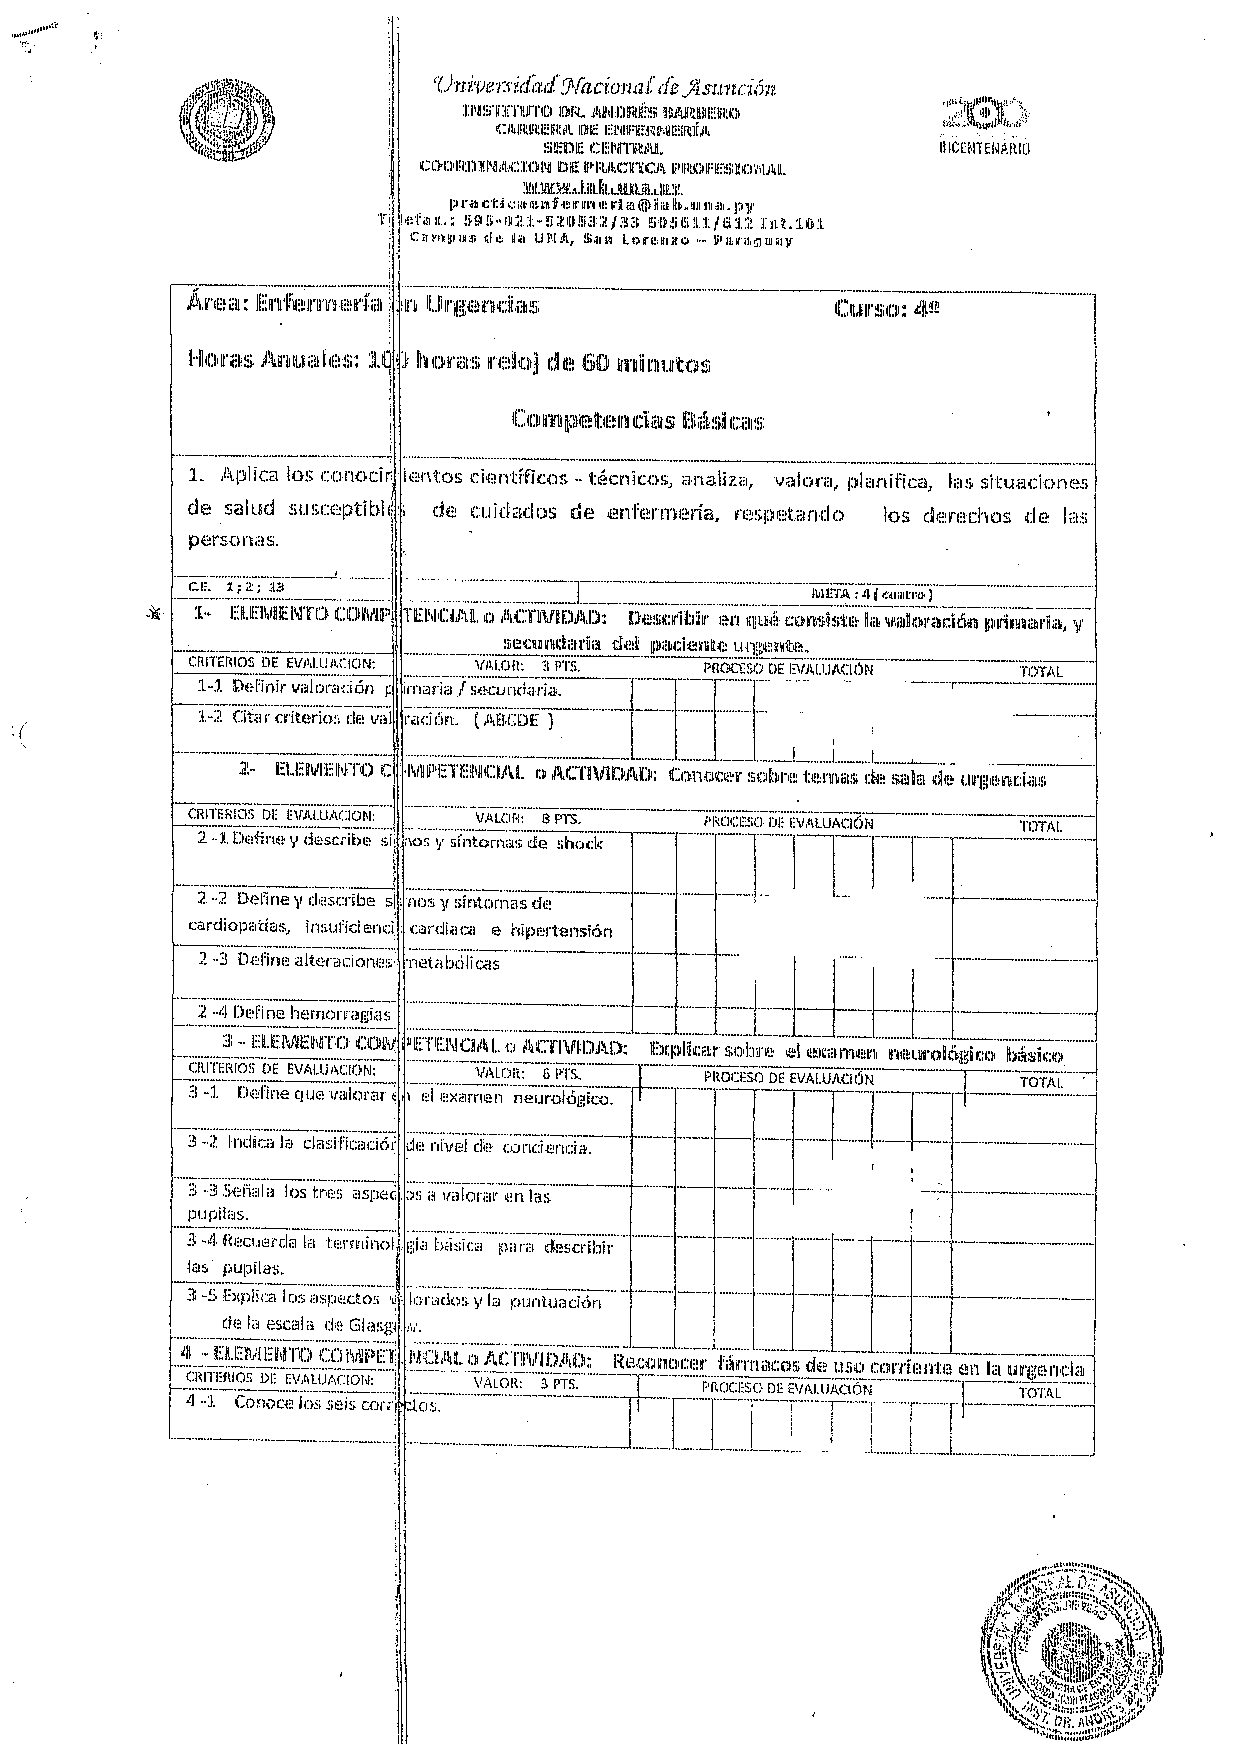
\includepdf[pages=1,scale=0.1]{anexo/documentos/planilla.pdf}
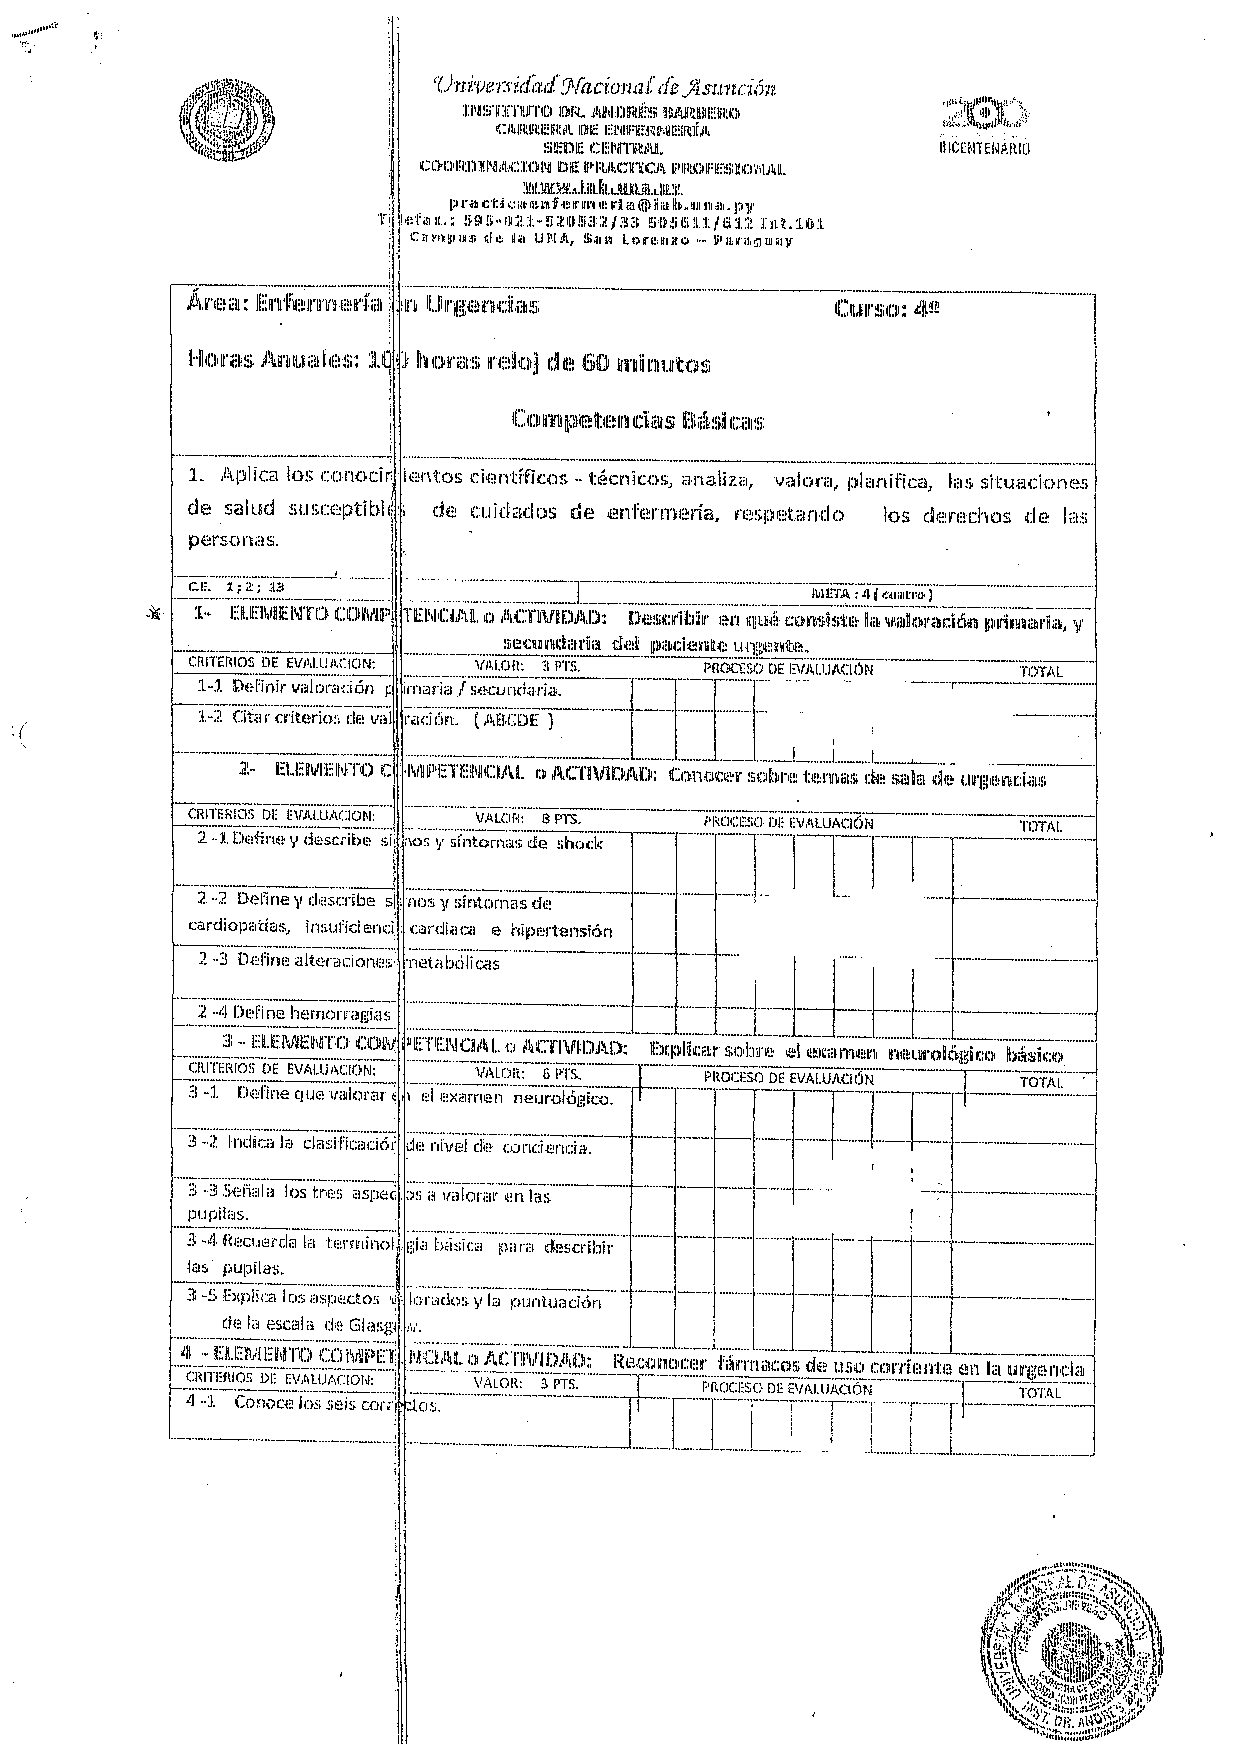
\includegraphics[scale=0.8]{anexo/documentos/planilla.pdf}
\includepdf[pages=2-4]{anexo/documentos/planilla.pdf}
\includepdf{anexo/documentos/planilla_h_5.pdf}
\includepdf[pages=6]{anexo/documentos/planilla.pdf}

\chapter{Reuniones}

\section{Reunión \#1}\label{reuniuxf3n-1}

\begin{itemize}
\itemsep1pt\parskip0pt\parsep0pt
\item
  \textbf{Fecha} 12 de Diciembre de 2013
\item
  \textbf{Presentes} Miguela Hermosilla, Arturo Volpe, Mirta González
\item
  \textbf{Motivo} Presentación de propuesta y búsqueda de apoyo.
\item
  \textbf{Lugar} Secretaría de la carrera de Enfermería, Instituto
  Andrés Barbero
\end{itemize}

\subsection{Objetivos}\label{objetivos}

\begin{itemize}
\itemsep1pt\parskip0pt\parsep0pt
\item
  Presentar idea de tésis
\item
  Presentar la idea como un complemento a la educación actual
\item
  Investigar posibles áreas de aplicación de la idea
\item
  Investigar mecanismos de medición
\item
  Validación de la investigación previa.
\end{itemize}

\subsection{Desarrollo}\label{desarrollo}

Los interesados se presentaron en la secretaría del Instituto Andes
Barbero (IAB), para poder hablar con la directora de la carrera, la que
se presento como Mgs. Miguela Hermosilla.

Se procedió a la explicación de los objetivos y deseos por parte de los
interesados, Miguela parecía muy interesada y dispuesta a ayudar, los
puntos claves que menciono son:

\begin{itemize}
\itemsep1pt\parskip0pt\parsep0pt
\item
  No se debe enfocar como la utilización de redes Sociales, pues el IAB
  no promueve la utilización de las mismas por problemas internos.
\item
  Los alumnos del 1ero y 2do año tienen un laboratorio especializado
  donde realizan pruebas empíricas con muñecos, incluso deben pasar
  exámenes prácticos antes de poder aprobar la materia con exámenes
  \textbf{teóricos}.
\item
  En el 3er año se realiza el primer contacto con los pacientes, en el
  cual tan solo dialogan con los pacientes.
\item
  En el 4to año los alumnos acceden a quirofano, ya teniendo experiencia
  previa con los muñecos.
\item
  Existen tesis de alumnos de enfermería que hablan de la utilización de
  la tecnología para facilitar la educación.
\item
  Existen dos tipos de examenes:

  \begin{itemize}
  \itemsep1pt\parskip0pt\parsep0pt
  \item
    Prácticos, donde los alumnos prueban con muñecos y un instructor se
    encarga de medir la pericia del mismo.
  \item
    Teóricos: a través de un examen \textbf{tradicional}
  \end{itemize}
\item
  Anualmente ingresan 150 nuevos estudiantes.
\item
  Los instructores utilizan elementos distractores en sus exámenes para
  poder medir la capacidad del alumno de detectar los temas que se
  consideran más importantes
\end{itemize}

\subsection{Recomendaciones sobre la
tesis}\label{recomendaciones-sobre-la-tesis}

\begin{itemize}
\itemsep1pt\parskip0pt\parsep0pt
\item
  La población recomendada para el estudio son los estudiante de 3er/4to
  año.
\item
  La forma de medición recomendada es dotar a un grupo la tecnología y
  utilizar otros dos como grupos de control.
\item
  Cada grupo tiene un conjunto de instructores que se encargan de
  enseñar y medir la capacidad del alumno.
\item
  Posibles áreas para la simulación:

  \begin{itemize}
  \itemsep1pt\parskip0pt\parsep0pt
  \item
    Cuidados críticos (pediatria, cuidado de adultos)
  \item
    Cirugía
  \item
    Traumatologia
  \end{itemize}
\item
  Además menciono (con ayuda de colegas), las áreas que más
  inconvenientes genera en alumnos:

  \begin{itemize}
  \itemsep1pt\parskip0pt\parsep0pt
  \item
    Bio-seguridad
  \item
    Preparación de drogas
  \item
    Difusión de drogas
  \item
    Ética
  \end{itemize}
\item
  Se puede empezar el estudio en abril, donde los grupos empiezan, se
  recomienda empezar con el 2do grupo , que empieza la segunda semana de
  abril y la medición se puede realizar en Junio. Los motivos de elegir
  el segundo grupo son:

  \begin{itemize}
  \itemsep1pt\parskip0pt\parsep0pt
  \item
    El primero no esta lo suficientemente preparado.
  \item
    El tiempo del tercer grupo se solapa con exámenes y los alumnos no
    están en peores condiciones..
  \end{itemize}
\end{itemize}

\subsection{Otras recomendaciones}\label{otras-recomendaciones}

\begin{itemize}
\itemsep1pt\parskip0pt\parsep0pt
\item
  Reunirnos con los instructores de cada grupo el día 20-12-2013 para
  presentar la idea y buscar apoyo
\item
  Investigar sobre las tesis relacionadas en el área para averiguar
  cuales son las áreas que más cuestan.
\item
  Enviar un mail para solicitar más información y confirmar la reunión
  con los instructores.
\end{itemize}

\subsection{Actividades}\label{actividades}

\begin{itemize}
\itemsep1pt\parskip0pt\parsep0pt
\item
  Enviar correo para verificar disponibilidad de instructores.
\item
  Decidir sobre cual tema se realizará el trabajo y notificar para que
  Miguela pueda ayudarnos.
\end{itemize}

\clearpage
\section{Reunión \#2}

\begin{itemize}
\itemsep1pt\parskip0pt\parsep0pt
\item
  \textbf{Fecha} 27 de Diciembre de 2013.
\item
  \textbf{Presentes} Miguela Hermosilla, Arturo Volpe, Mirta González.
\item
  \textbf{Motivo} Presentación de ítems pre-seleccionados y evaluación
  de los mismos por la Profesora Miguela Hermosilla.
\item
  \textbf{Lugar} Secretaría de la carrera de Enfermería, Instituto
  Andrés Barbero.
\end{itemize}

\subsection{Objetivos}

\begin{itemize}
\itemsep1pt\parskip0pt\parsep0pt
\item
  Obtener la valoración de un profesional de los elementos a simular.
\item
  Investigar en que materia aprenden a mezclar medicamentos.
\item
  Obtener una reunión con los instructores, pues serán ellos quienes
  realizarán las pruebas.
\end{itemize}

\subsection{Desarrollo}

Los interesados se presentaron en la secretaría del Instituto Andes
Barbero (IAB), para reunirse con la directora de la carrera, Mgs.
Miguela Hermosilla.

Se expusieron los items pre-seleccionados para la simulación con el fin
de que puedan ser valorados.

\subsubsection{Items presentados}

\begin{enumerate}
\def\labelenumi{\arabic{enumi}.}
\itemsep1pt\parskip0pt\parsep0pt
\item
  Interpretación de la escala de \emph{glasgow} (Enfermería en cuidados
  intensivos, 4to año).
\item
  Reanimación cardiopulmonar básica y avanzada, distinción de los
  fármacos más utilizados (Enfermería en cuidados intensivos, 4to año).
\item
  Test de \emph{apgar} (Pediatría, 3er año).
\item
  Mezcla y administración de fármacos.
\item
  Conocimiento de las normas y medidas prácticas referentes a la
  bioseguridad.
\end{enumerate}

\textbf{Además se consultaron los siguientes puntos:}

\begin{enumerate}
\def\labelenumi{\arabic{enumi}.}
\itemsep1pt\parskip0pt\parsep0pt
\item
  Identificación de las características anatómicas y fisiológicas del
  recién nacido (Salud del niño y del adolescente, 3er año).
\item
  Demostrar destreza en la atención inmediata del recién nacido (Salud
  del niño y del adolescente, 3er año).
\end{enumerate}

\subsection{Recomendaciones del
profesional}

\begin{enumerate}
\def\labelenumi{\arabic{enumi}.}
\itemsep1pt\parskip0pt\parsep0pt
\item
  Este ítem puede ser aplicado para los alumnos del 3er o 4to año. Posee
  práctica. \textbf{Su orden de importancia es 3.}
\item
  Este ítem puede ser aplicado para los alumnos del 3er o 4to año.
  \textbf{Su orden de importancia es 1}, esto es debido a que este ítem
  tiene cero práctica en la actualidad, por que, la malla curricular no
  cuenta con temas relacionados a los primeros auxilios.
\item
  Este ítem posee prácticas, sin embargo, enfermería sólo se encargaría
  de la valoración del test. Puede ser aplicado para los alumnos del 3er
  o 4to año. \textbf{Su orden de importancia es 4}.
\item
  Este ítem no necesita pericia. Puede ser aplicado para los alumnos del
  3er año. \textbf{Su orden de importancia es 5.}
\item
  Este ítem se considera transversal, es decir, bioseguridad es
  importante en cada procedimiento. Incluye: protección, lavado de
  manos, asepsia, anti-sepsia. Es el que más práctica tiene. Puede ser
  aplicado para alumnos de 3er año. \textbf{Su orden de importancia es
  2}.
\end{enumerate}

\emph{Cabe mencionar que el orden de importancia del ítem va de 1 a 5,
siendo el 1 el indicador de mayor valor.}

\textbf{En cuanto a los demás puntos, mencionó:}

\begin{enumerate}
\def\labelenumi{\arabic{enumi}.}
\itemsep1pt\parskip0pt\parsep0pt
\item
  Este ítem está incluido en 2 (Reanimación cardiopulmonar). Puede ser
  aplicado para los alumnos del 4to año.
\item
  Este ítem depende de a que se refiera, puede referirse a:

  \begin{itemize}
  \itemsep1pt\parskip0pt\parsep0pt
  \item
    la recepción del recién nacido,
  \item
    instalación de un vía,
  \item
    instalación de sonda nasogástrica.
  \end{itemize}

  Puede ser aplicado para alumnos del 4to año. Su nivel de complejidad
  depende del punto que se tome en cuenta, así como el enfoque del
  mismo. Por ejemplo, la \texttt{recepción de un recién nacido} es un
  conocimiento importante pero con el cual se cuenta práctica, en cambio
  la \texttt{instalación de una vía} es un proceso sumamente complejo,
  que no cuenta con práctica.
\end{enumerate}

\subsection{Otras informaciones}

\begin{itemize}
\itemsep1pt\parskip0pt\parsep0pt
\item
  Todas las pericias son evaluadas por un instructor.
\item
  Existen 4 estudiantes por instructor en las áreas críticas (cuidados
  intensivos, urgencias). Un área critica es aquella en la cual el
  paciente depende exclusivamente de un procedimiento externo.
\item
  Existen 10 estudiantes por instructor en las áreas no críticas.
\item
  Los instructores definen las cosas que evalúan. Cuentan con una
  planilla por alumnos para el seguimiento de las pericias (si son
  logradas o no, incluye los procedimientos).
\item
  Los instructores no están en enero.
\item
  La Sra. Miguela Hermosilla se encontrará en las instalaciones del
  Instituto Andrés Barbero del 6 al 10 de enero de 8:00 a 13:00 horas.
  Debemos reunirnos en alguna de estas fechas con ella para que nos
  pueda presentar a algún instructor que se encuentre, con el fin de que
  podamos reunirnos con él.
\end{itemize}

\subsection{Conclusiones}

\begin{itemize}
\itemsep1pt\parskip0pt\parsep0pt
\item
  Programar una reunión con los instructores, para ello se puede
  utilizar los días que la profesora Miguela no este de vacaciones y
  pedir su ayuda como contacto directo (si existe algún instructor
  presente).
\item
  Obtener la validación de un instructor acerca de los elementos a
  simular.
\end{itemize}

\clearpage
\section{Reunión \#3}\label{reuniuxf3n-3}

\begin{itemize}
\itemsep1pt\parskip0pt\parsep0pt
\item
  \textbf{Fecha} 08 de Enero de 2014.
\item
  \textbf{Presentes} Prof.~Gloria Mora, Arturo Volpe, Mirta González.
\item
  \textbf{Motivo} Primer encuentro con un instructor
\item
  \textbf{Lugar} MECIP, Instituto Andrés Barbero.
\end{itemize}

\subsection{Objetivos}\label{objetivos}

Reunión con instructores para obtener su valoración acerca de los ítems
pre-seleccionados para simular, la situación actual de los alumnos de
enfermería y otras informaciones relevantes que nos pueda brindar.

\subsection{Desarrollo}\label{desarrollo}

Los interesados acudieron a la Secretaría de la carrera de Enfermería en
el Instituto Andrés Barbero, donde fueron guiados por una secretaría
hasta el MECIP, donde se llevo a cabo la reunión con la profesora Gloria
Mora.

Los alumnos presentaron la propuesta y los ítems pre-seleccionados hasta
el momento.

La profesora Gloria Mora, es instructora en la materia ``Enfermería de
Urgencias'', encargada de los alumnos que atienden adultos que van al
hospital de Emergencias Médicas.

\subsubsection{Comentarios de la
profesora}\label{comentarios-de-la-profesora}

\begin{itemize}
\itemsep1pt\parskip0pt\parsep0pt
\item
  Enfermería en urgencias es una materia de cuarto curso, y se basa en
  tres competencias básicas, entre las cuales se encuentra el control de
  los signos vitales (frecuencia cardíaca, frecuencia respiratoria,
  presión arterial y temperatura).
\item
  La profesora es encargada de los alumnos durante 4 semanas, las cuales
  organiza como sigue:

  \begin{itemize}
  \itemsep1pt\parskip0pt\parsep0pt
  \item
    1 semana de prácticas en el laboratorio, si bien, según otras
    profesoras, los alumnos deben estar completamente preparados para
    las prácticas, Gloria menciona que prefiere una semana más bajo su
    supervisión para que los alumnos sepan como actuar y entiendan el
    lenguaje en el que se comunicará durante las prácticas.
  \item
    1 Semana donde la profesora guía a los alumnos en sus actividades,
    considera a esta semana como de conocimiento, exploración y
    adaptación al ambiente.
  \item
    2 Semanas durante las cuales vigila el desenvolvimiento de los
    alumnos y corrige sus actividades, al mismo tiempo que evalúa la
    pericia.
  \end{itemize}
\item
  Existe software que se utiliza para la instalación del catéter de PIC,
  de monitoreo y de soporte.
\item
  Control de los signos vitales:

  \begin{itemize}
  \itemsep1pt\parskip0pt\parsep0pt
  \item
    \textbf{Primarias}, son el control de los signos vitales, lo que
    menciono se llama el ABCDE de los signos vitales.
  \item
    \textbf{Secundarias}, la piel y daños secundarios.
  \end{itemize}
\end{itemize}

\paragraph{Evaluación}\label{evaluaciuxf3n}

Los alumnos del 4to curso de la materia \emph{Enfermería en Urgencias},
distribuyen la práctica como sigue:

\begin{itemize}
\itemsep1pt\parskip0pt\parsep0pt
\item
  Centro de emergencias médicas, 4 semanas, aquí es donde la profesora
  es la instructora. En este lugar atienden pacientes con accidentes y/o
  agresiones.
\item
  Urgencias en el Hospital de Clínicas, 4 semanas. En este lugar
  atienden pacientes crónicos y agudos.
\end{itemize}

Las prácticas tienen una duración de 4 horas, y son llevadas a cabo de
las 13 hasta las 17 horas (4 horas por día).

Algunas actividades que se evalúan son por ejemplo:

\begin{itemize}
\itemsep1pt\parskip0pt\parsep0pt
\item
  Posicionamiento del paciente al a hora de hacer tratamientos
  (elevación de piernas, posicionamiento de la cabeza)
\item
  Valoración del paciente (ABCDE)
\item
  Toma de sangre
\end{itemize}

Además nos entrego una copia de la hoja de evaluación, la cual es
completada por la misma para cada alumno, en la hoja se constatan las
competencias básicas y la progresión de los procedimientos en los
alumnos.

\paragraph{Tipos de alumnos}\label{tipos-de-alumnos}

\begin{itemize}
\itemsep1pt\parskip0pt\parsep0pt
\item
  \textbf{Desinteresado}, no muestra interés y escapa conscientemente de
  las prácticas. (\textasciitilde{}25\%)
\item
  \textbf{Introvertido}, es difícil que ayude, pero una vez que empieza
  a ayudar siempre ayuda sin problemas (\textasciitilde{}25\%)
\item
  \textbf{Extrovertidos}, ayudan sin problemas y se muestran interesados
  ante las enseñanzas, sienten que aplican la teoría
  (\textasciitilde{}50\%).
\end{itemize}

\paragraph{Tecnología}\label{tecnologuxeda}

Los alumnos deben estar familiarizados con las máquinas que sirven para
medir diferentes aspectos del estado de un paciente, y los que se
utilizan para diferentes tratamientos (como ejemplo un desfribilador).

Además, tienen permitido utilizar el celular siempre y cuando no estén
en la sala (pueden ir al baño, en la sala de descansos o cuando tienen
tiempo para comer).

\subsubsection{Otros}\label{otros}

Ante consultas sobre los elementos seleccionados, mostró un especial
interés por la escala de glasgow.

\clearpage
\section{Reunión \#4}\label{reuniuxf3n-4}

\begin{itemize}
\itemsep1pt\parskip0pt\parsep0pt
\item
  \textbf{Fecha} 08 de Mayo de 2014.
\item
  \textbf{Presentes} Prof.~Miguela Hermosilla, Arturo Volpe, Mirta
  González y Prof Matilde (laboratorio)
\item
  \textbf{Motivo} Presentación de laboratorios de prácticas
\item
  \textbf{Lugar} Secretaría general del departamento de enfermería y
  laboratorios de prácticas de estudiantes de enfermería y obstetricia.
\end{itemize}

\subsection{Objetivos}\label{objetivos}

\begin{itemize}
\itemsep1pt\parskip0pt\parsep0pt
\item
  Validación de la navegación actual de la simulación.
\item
  Exploración de los laboratorios y observación de prácticas actuales de
  los estudiantes de enfermería.
\end{itemize}

\subsection{Desarrollo}\label{desarrollo}

La reunión se llevo a cabo en dos partes:

\subsubsection{Primera reunión}\label{primera-reuniuxf3n}

La primera reunión se llevo a cabo en la secretaría de la carrera de
enfermería y cumplió con el primer objetivo, la validación de la
navegación actual.

\paragraph{Observaciones}\label{observaciones}

\begin{itemize}
\itemsep1pt\parskip0pt\parsep0pt
\item
  Es necesario un acceso directo a la parte específica del cuerpo donde
  se esta
\item
  Sala:

  \begin{itemize}
  \itemsep1pt\parskip0pt\parsep0pt
  \item
    En general, Es necesario más realismo en la escena de la simulación.
  \item
    Agregar ventanas con los colores típicos de un hospital (amarillos,
    ver fotos de la segunda reunión) realizando la práctica.
  \end{itemize}
\item
  Camilla:

  \begin{itemize}
  \itemsep1pt\parskip0pt\parsep0pt
  \item
    Eliminar las barandas de la camilla actual (mientras más sencilla la
    camilla mejor)
  \item
    La camilla debe estar más alta.
  \end{itemize}
\item
  Pacientesente:

  \begin{itemize}
  \itemsep1pt\parskip0pt\parsep0pt
  \item
    Remera mangas cortas
  \item
    Sin Anteojos
  \end{itemize}
\item
  Simulación:

  \begin{itemize}
  \itemsep1pt\parskip0pt\parsep0pt
  \item
    Tomar en cuenta la presión de la sangre
  \end{itemize}
\end{itemize}

\subsubsection{Segunda reunión}\label{segunda-reuniuxf3n}

La segunda reunión se llevo a cabo en los laboratorios de enfermaría con
la Prof Matilde, la cual es profesora de laboratorio del primer semestre
de la carrera de enfermería, se nos presentaron tres laboratorios, los
dos primeros de arquitectura similar pero diferente propósito, el
primero es un laboratorio/sala convertido en un aula donde los alumnos
observan maquetas muy detalladas del cuerpo humano y tienen sus primeras
prácticas bajo supervisión de un profesor.

La segunda sala es un laboratorio/sala que cuenta con numerosas camas
donde los alumnos práctican todo lo referente al mantenimiento adecuado
de las camas, cuenta además con maniquís que los estudiantes utilizan
para interactuar con un cuerpo, el mismo tiene una contextura similar al
de un cuerpo humano y varias partes marcadas con alertas visuales sobre
puntos de referencia, como por ejemplo donde se debe vacunar, donde se
debe realizar la reanimación, donde están las venas donde se pueden
ingresar vías, etc.

La tercera sala es un laboratorio de obstetricia, en el cual se pueden
ver varios maniquíes de bebes y partes sexuales de la mujer, todo lo
necesario para poder simular un parto.

\paragraph{Observaciones}\label{observaciones-1}

\begin{itemize}
\itemsep1pt\parskip0pt\parsep0pt
\item
  Los alumnos en el primer laboratorio observan, tocan y palpan los
  brazos falsos para poder saber donde están las venas importantes para
  la instalación de vías. Aquí además aprenden donde se deben ubicar
  cuando se acercan a un paciente, donde debe estar el lugar estéril
  para depositar los elementos y como preparar el equipo necesario.
\item
  El segundo laboratorio además cuenta con esterilizadores, donde los
  alumnos aprenden conceptos básicos sobre la esterilización (la teoría
  se da en otra materia), aquí más bien se manipula el esterilizador
\item
  Existen varios tipos de vías que pueden ser utilizados para una vena,
  y cada vena a su vez es capaz de aguantar ciertos tipos de vías,
  siendo las venas de las manos las que requieren vías más pequeñas. El
  único tipo de vía que no es colocado por el enfermero es la vía
  central (requiere de un anestesiologo).
\end{itemize}





\printbibliography{}


\end{document}
